\appendix
\section{Appendix}

\subsection{Settings}
\begin{table}[h!]
  \centering
  \begin{tabular}{ll}
  Device & Delay \\\toprule[1.5pt]
  TSCA for NaI & $1.00$ (minimal setting) at $0.1-1.1\mu \mathrm{s}$ \\
  TSCA for PVC & $2.20$ at $1-11\mu \mathrm{s}$\\
  Delay unit NaI & $3.25\mu \mathrm{s}$\\
  Delay unit PVC & $3.75\mu \mathrm{s}$ \\\bottomrule[1.5pt]
  \end{tabular}
  \caption{Delay settings.}
  \label{tab:delays}
\end{table}

\begin{table}[h!]
  \centering
  \begin{tabular}{lll}
  Device & Coarse Gain & Fine Gain \\\toprule[1.5pt]
  NaI amplifier & 16 & 6.5 \\
  PVC amplifier & 8 & 6.0\\ \bottomrule[1.5pt]
  \end{tabular}
  \caption{Amplification settings.}
  \label{tab:amps}
\end{table}

\FloatBarrier
\subsection{Energy Calibration}

\begin{figure}[h!]
  \centering
  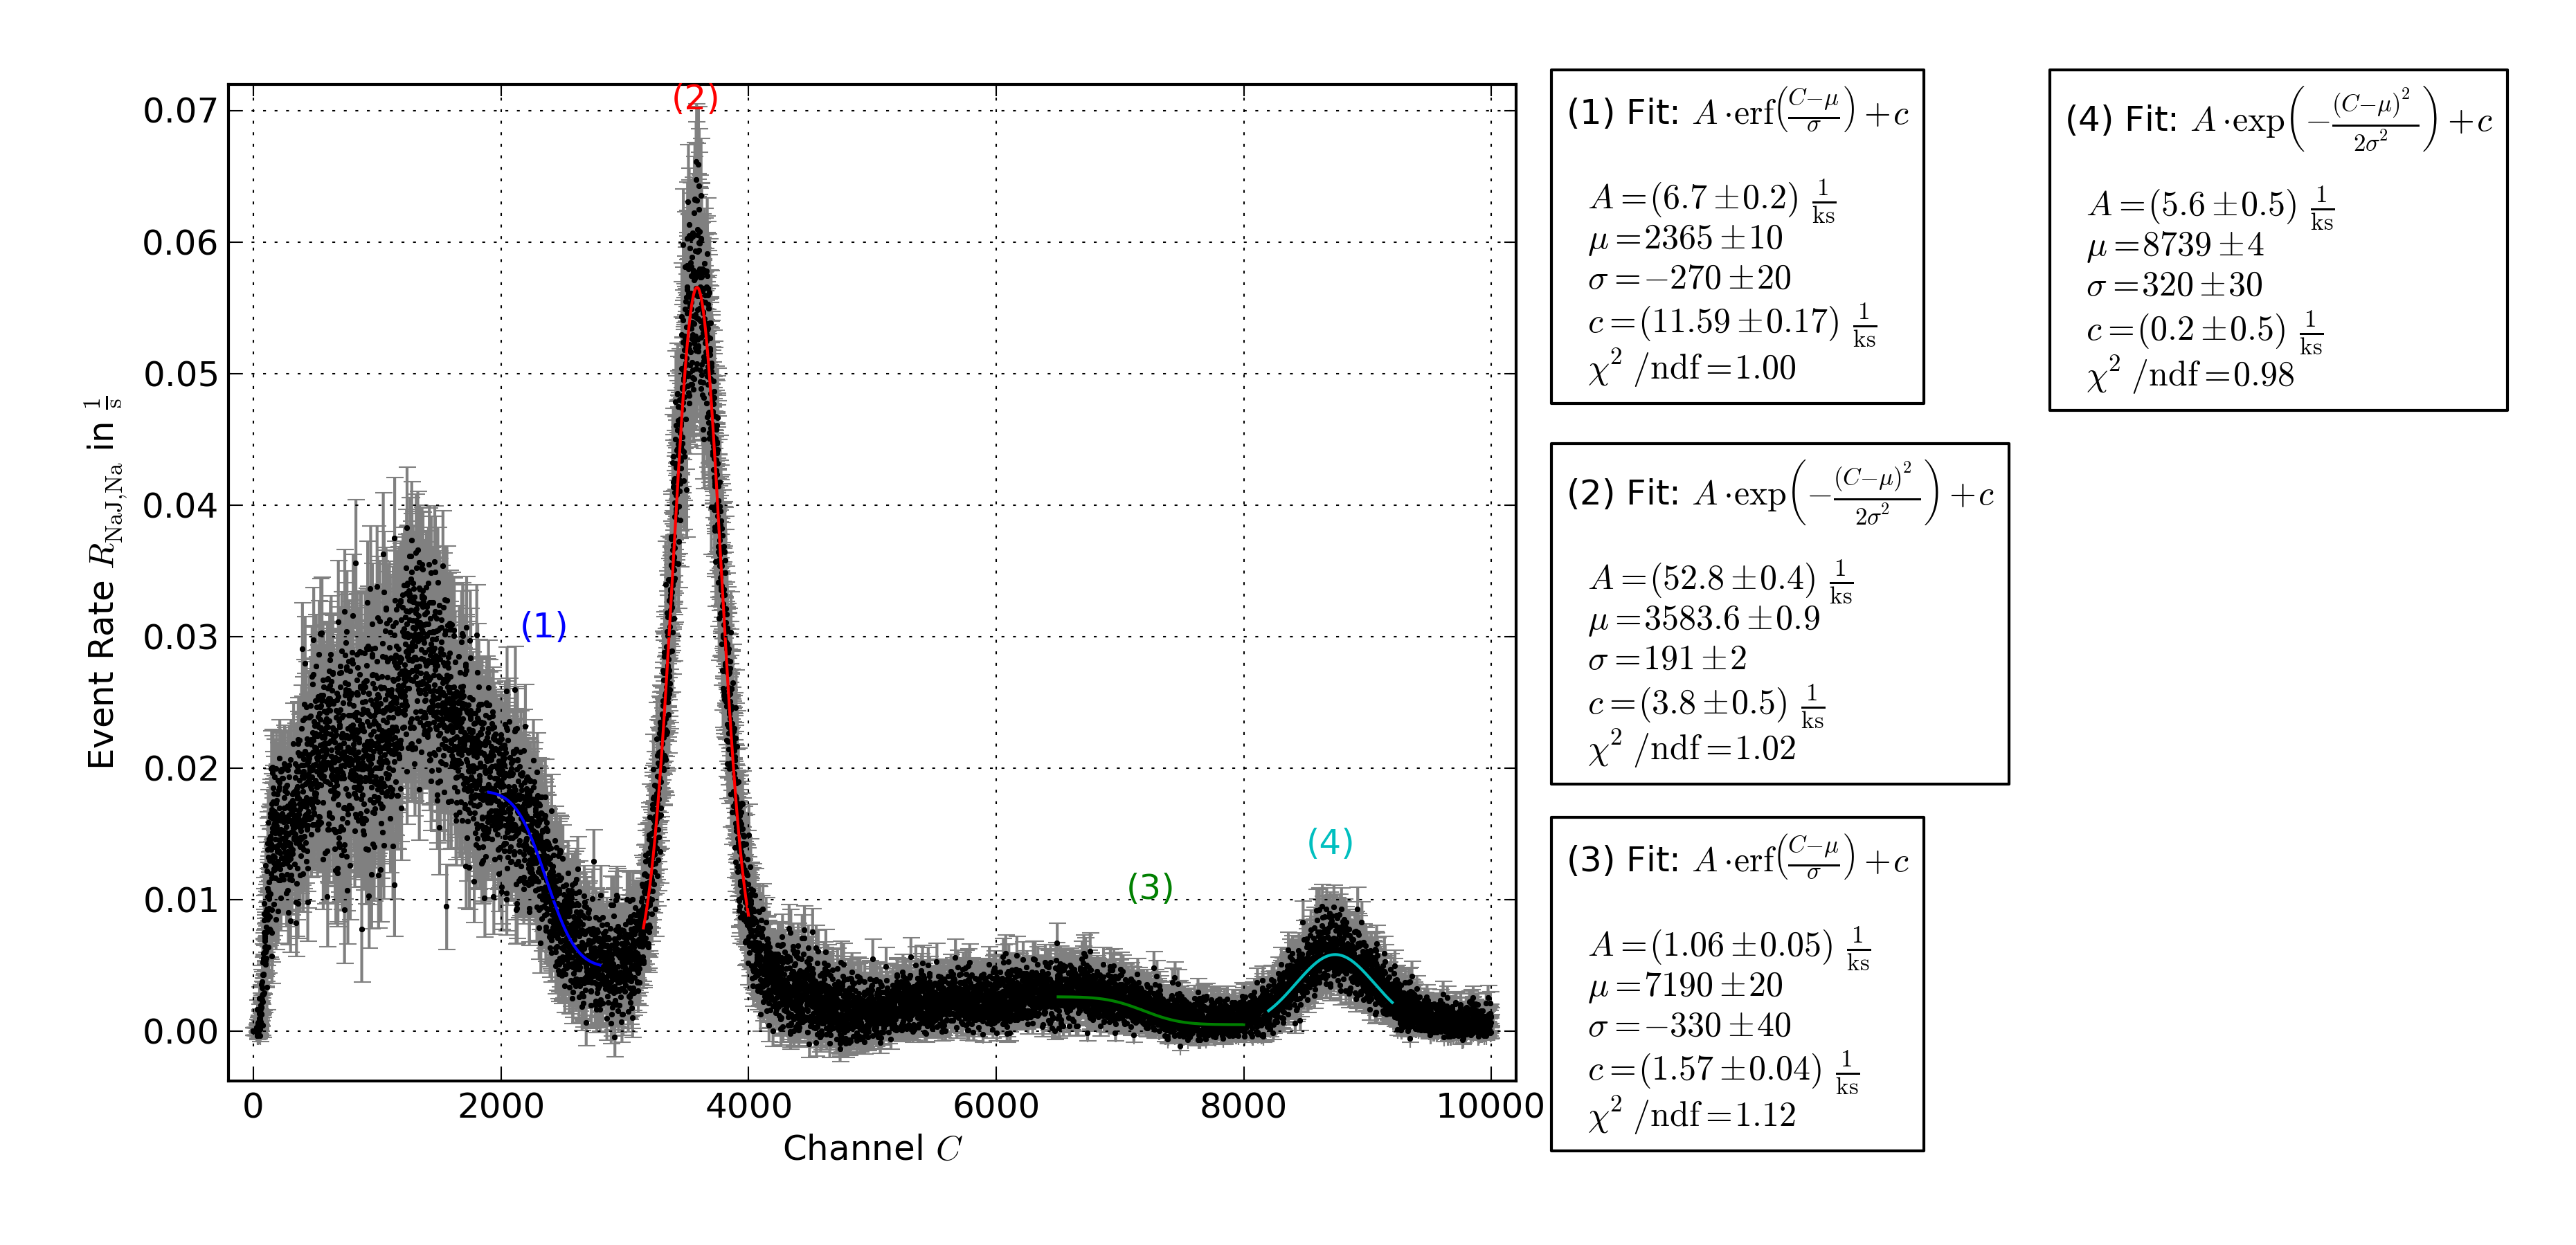
\includegraphics[width=1.0\textwidth]{plots/naj_na.png}
  \caption{Background revised decay spectrum of \Na measured with the NaI
  scintillator. Certain peaks and edges are fitted with the corresponding
  function. The gray area corresponds to the error bars. Measurement
  duration $t=3600\mathrm{s}$.}
  \label{fig:calibNaJNa}
\end{figure}

\begin{figure}[h!]
  \centering
  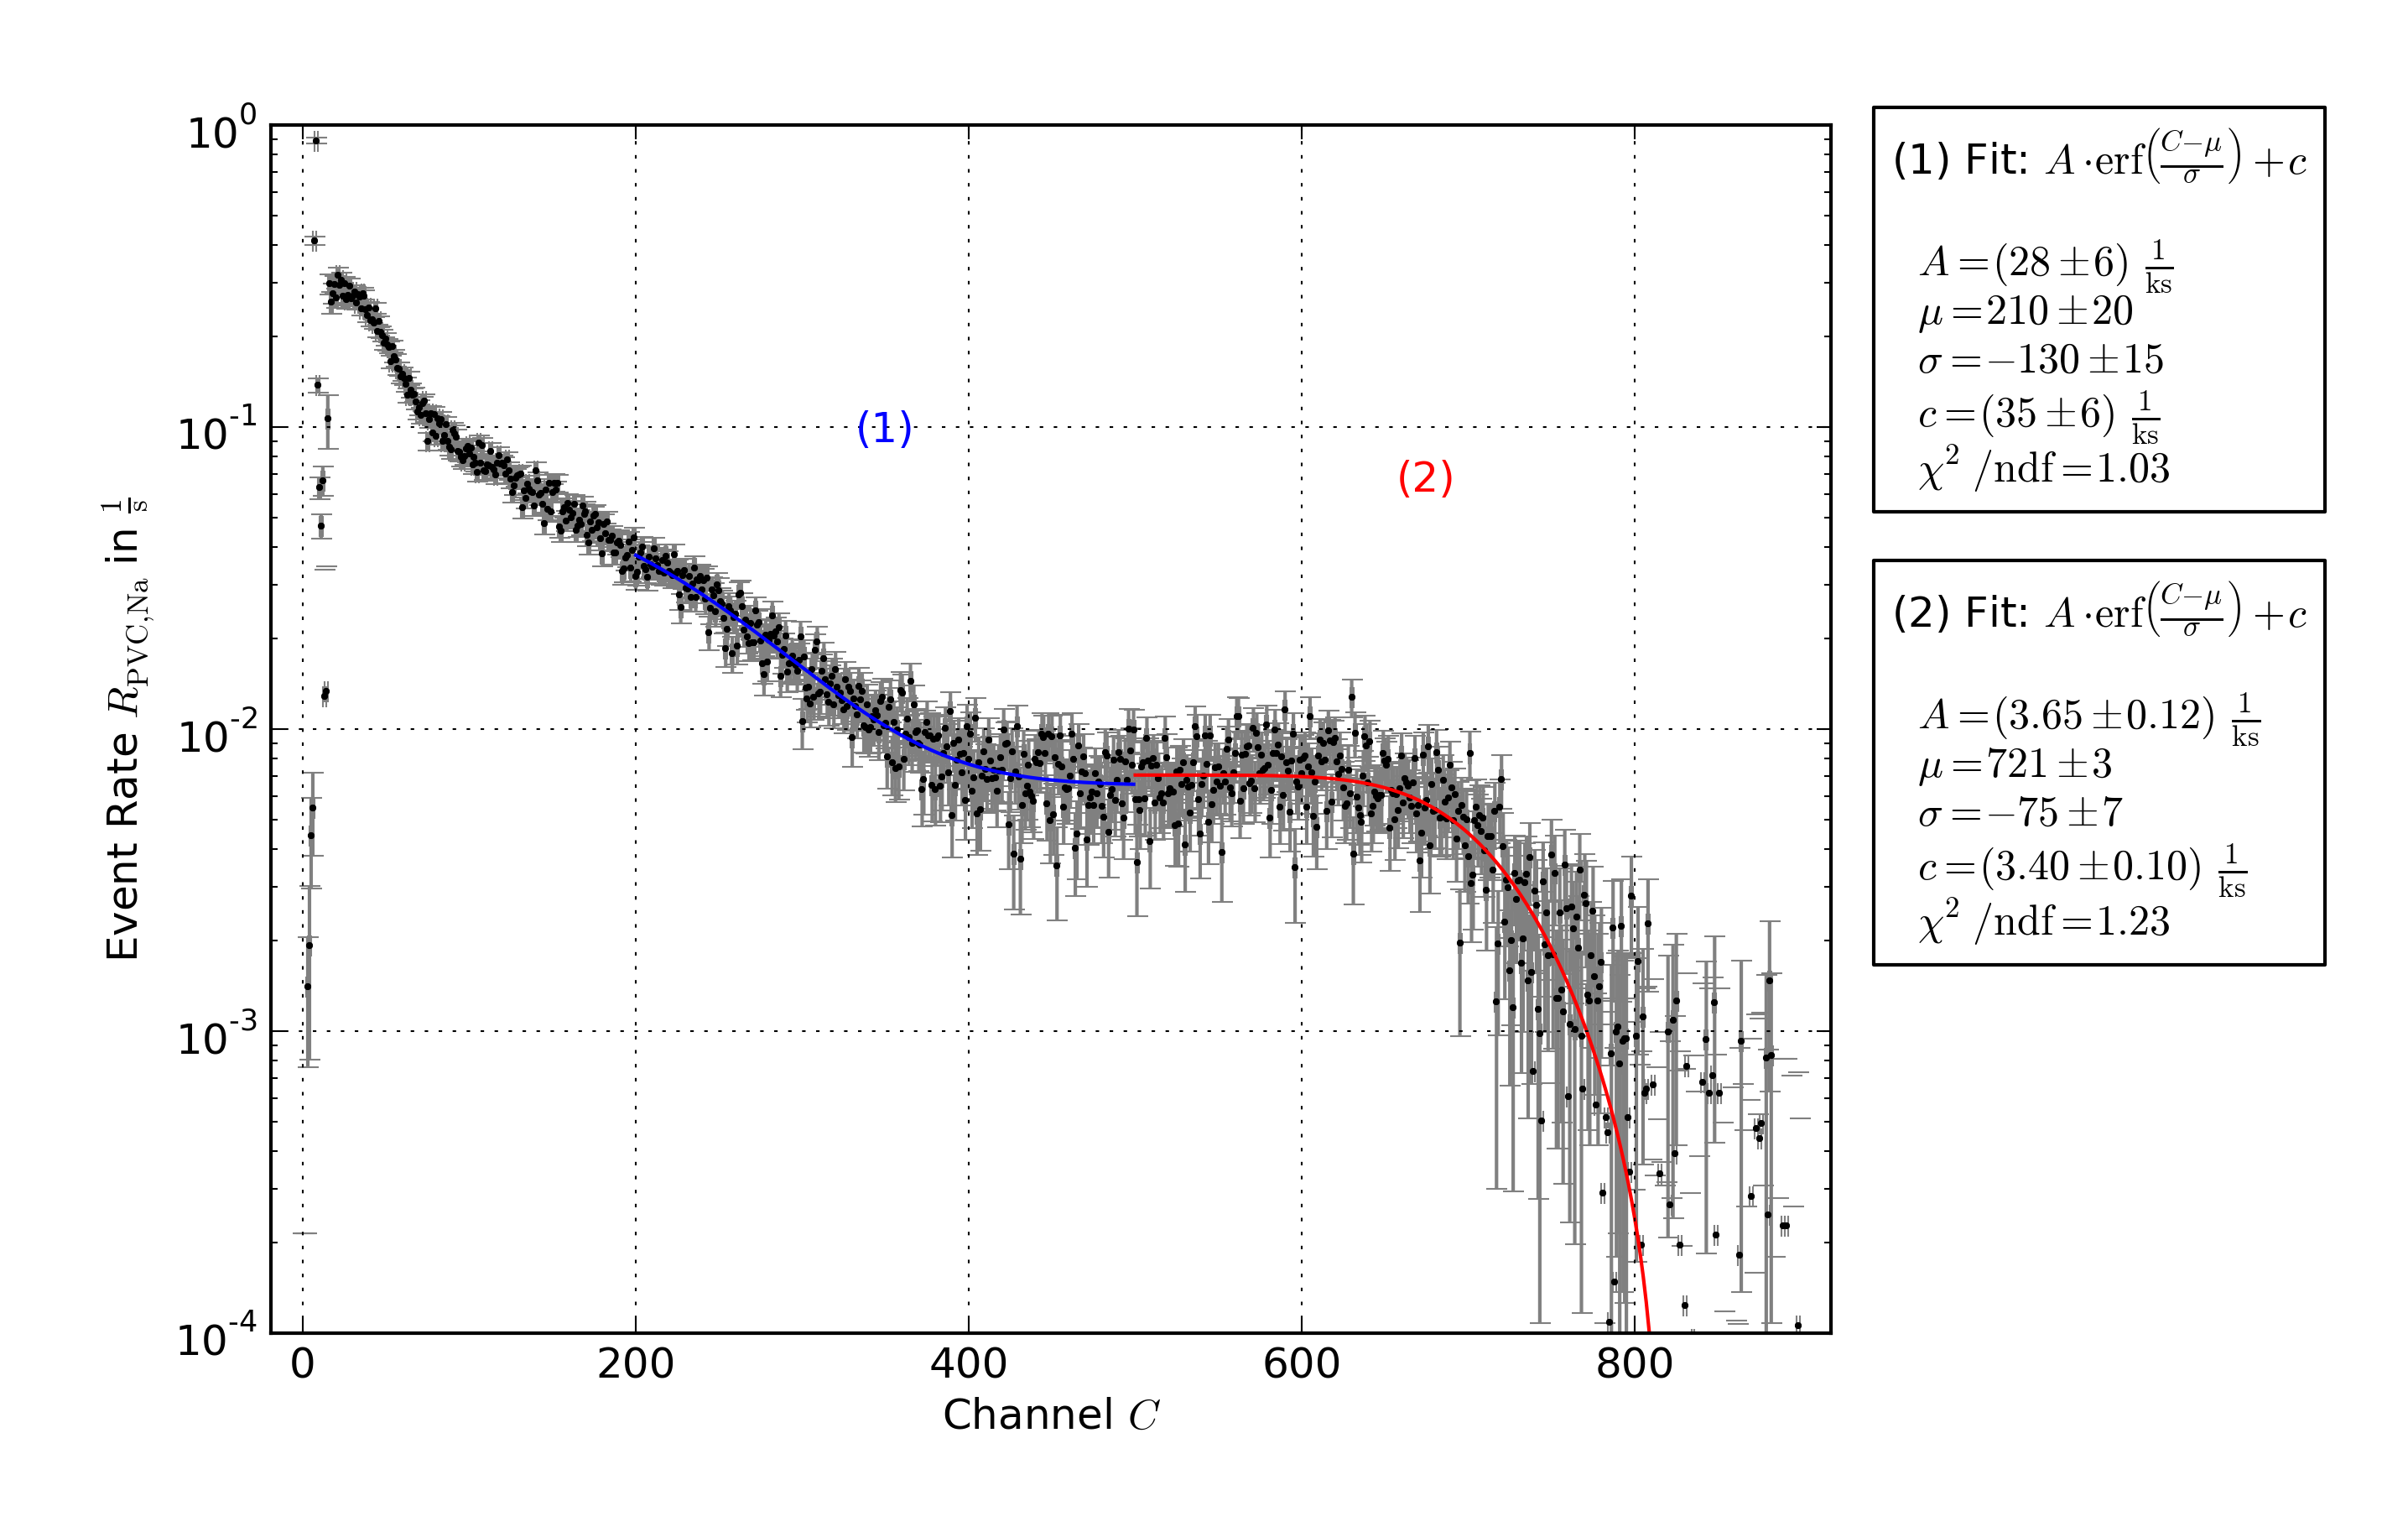
\includegraphics[width=1.0\textwidth]{plots/pvc_na.png}
  \caption{Background revised decay spectrum of \Na measured with the PVC
  scintillator. Certain peaks and edges are fitted with the corresponding
  function. The gray area corresponds to the error bars. Measurement
  duration $t=4197.6\mathrm{s}$.}
  \label{fig:calibPVCNa}
\end{figure}

\begin{figure}[h!]
  \centering
  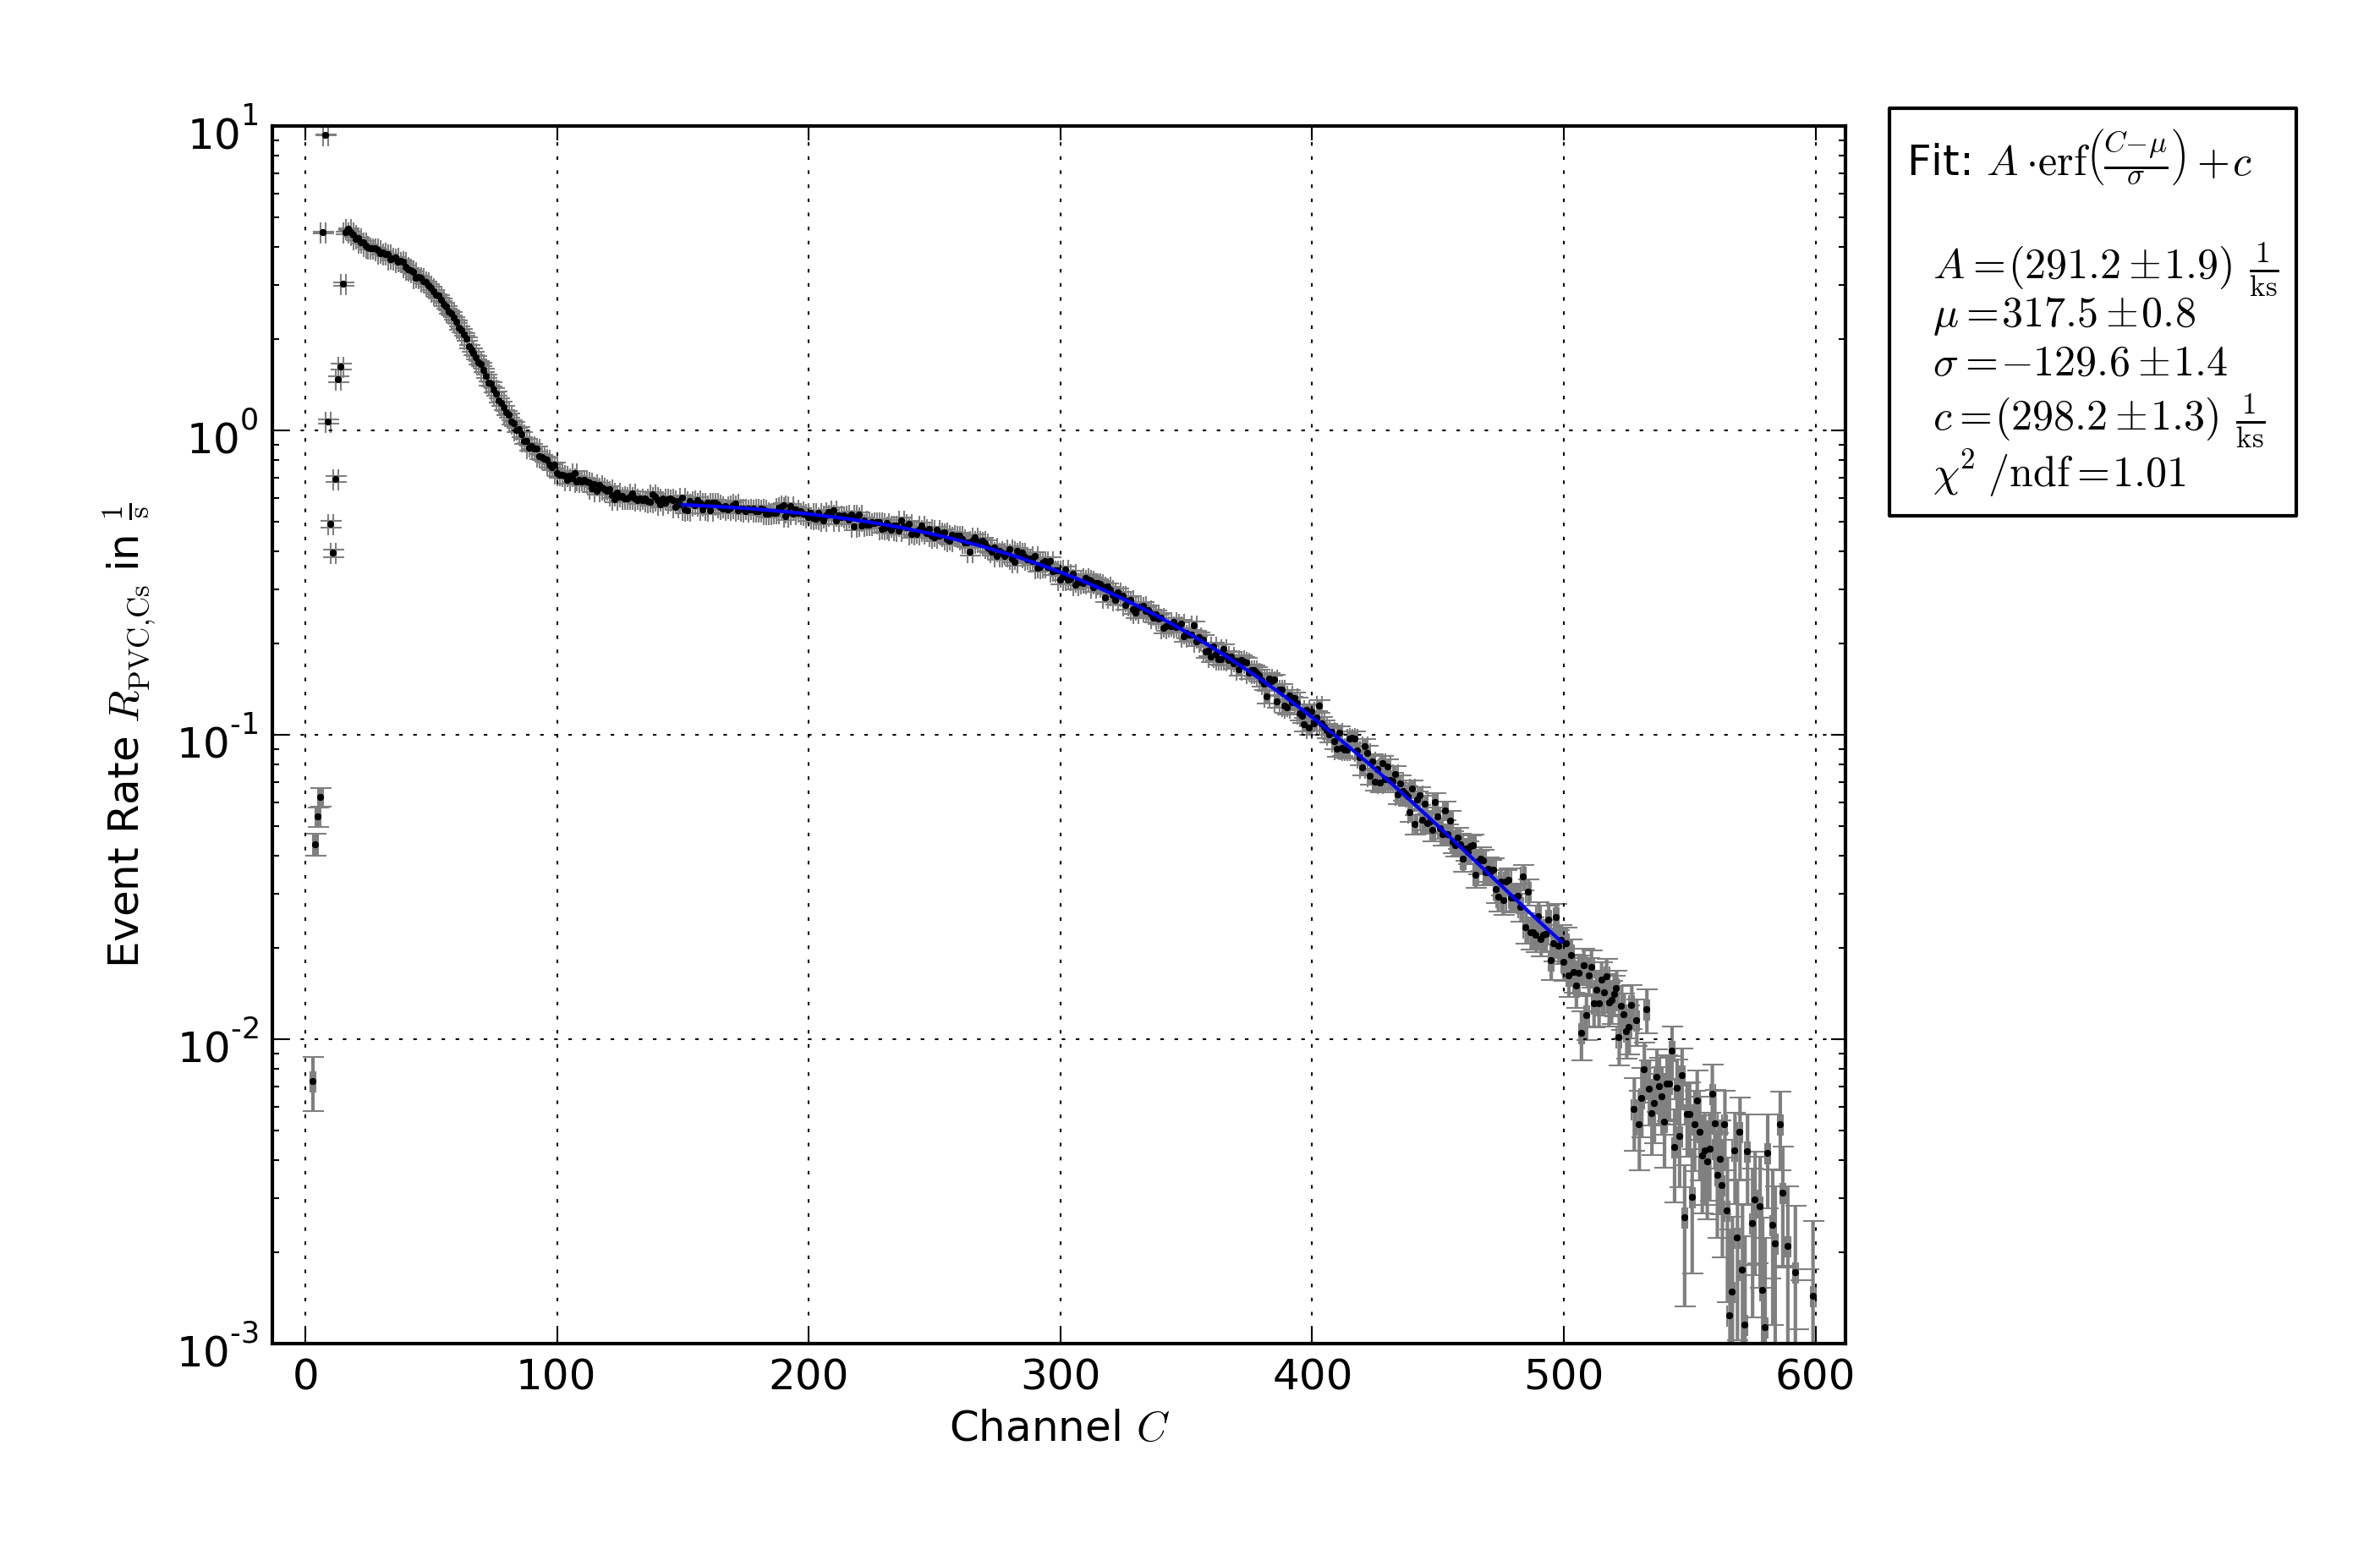
\includegraphics[width=1.0\textwidth]{plots/pvc_cs.png}
  \caption{Background revised decay spectrum of \Cs measured with the PVC
  scintillator. Certain peaks and edges are fitted with the corresponding
  function. The gray area corresponds to the error bars. Measurement
  duration $t=3600.9\mathrm{s}$.}
  \label{fig:calibPVCCs}
\end{figure}

\begin{table}[htb]
  \centering
  \begin{tabular}{rclcl}
  Source & Energy in $\mathrm{keV}$ & Type & Fit \# & Channel $C$
  \\\toprule[1.5pt]
  \Cs & 477 & \compton edge & 1 & $\pyexp{calib_pvc_cs_1}$\vspace{0.3em}\\
  \Na & 341 & \compton edge & 1 &  $\pyexp{calib_pvc_na_1}$\\ 
   & 1064 & \compton edge & 2 &  $\pyexp{calib_pvc_na_2}$\\\bottomrule[1.5pt]
  \end{tabular}
  \caption{Assignment of fitted peaks and edges to the known energies
  \cite{anleitung} for the PVC scintillator.}
  \label{tab:assignmentPVC}
\end{table}

\FloatBarrier
\subsection{Conservation of Energy}
\subsubsection{Organic Scintillator}
\begin{figure}[h!]
  \centering
  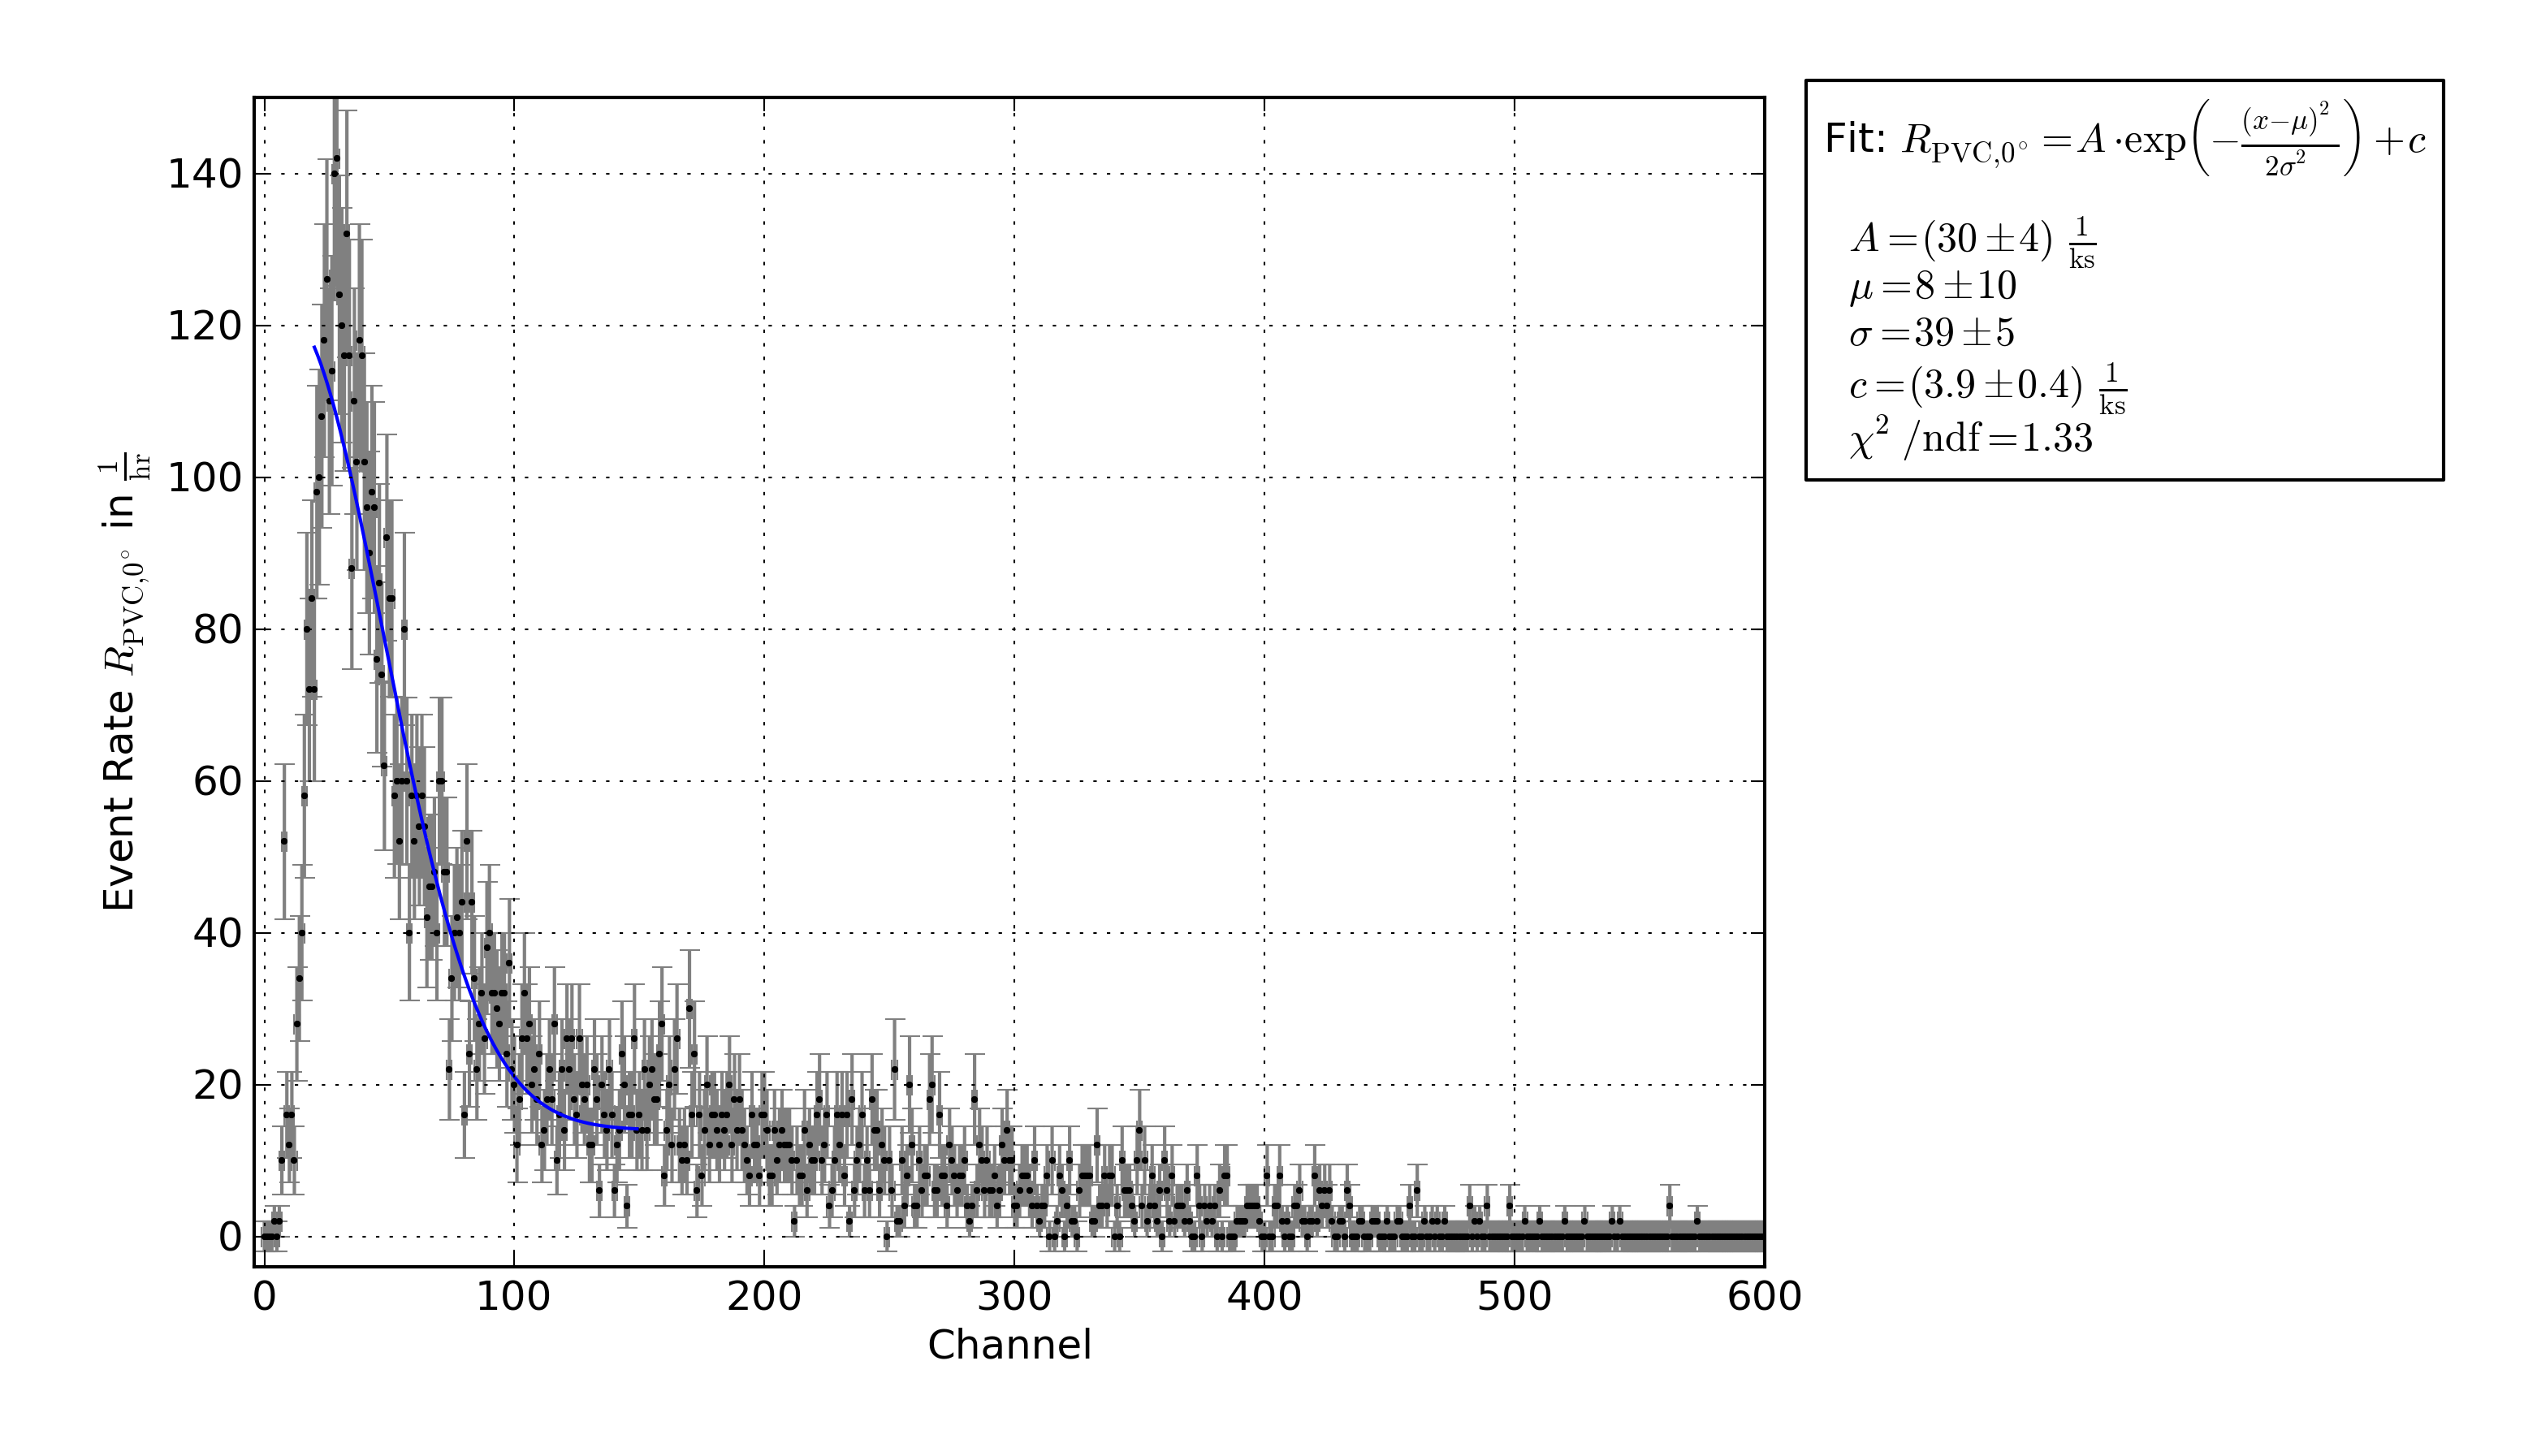
\includegraphics[width=0.6\textwidth]{plots/pvc_0.png}
  \caption{Electron energy spectrum (PVC scintillator) of coincident signals
  with $\theta=0\degree$. Measurement duration $t=1880.27{s}$.}
  \label{fig:pvc0}
\end{figure}
\begin{figure}[h!]
  \centering
  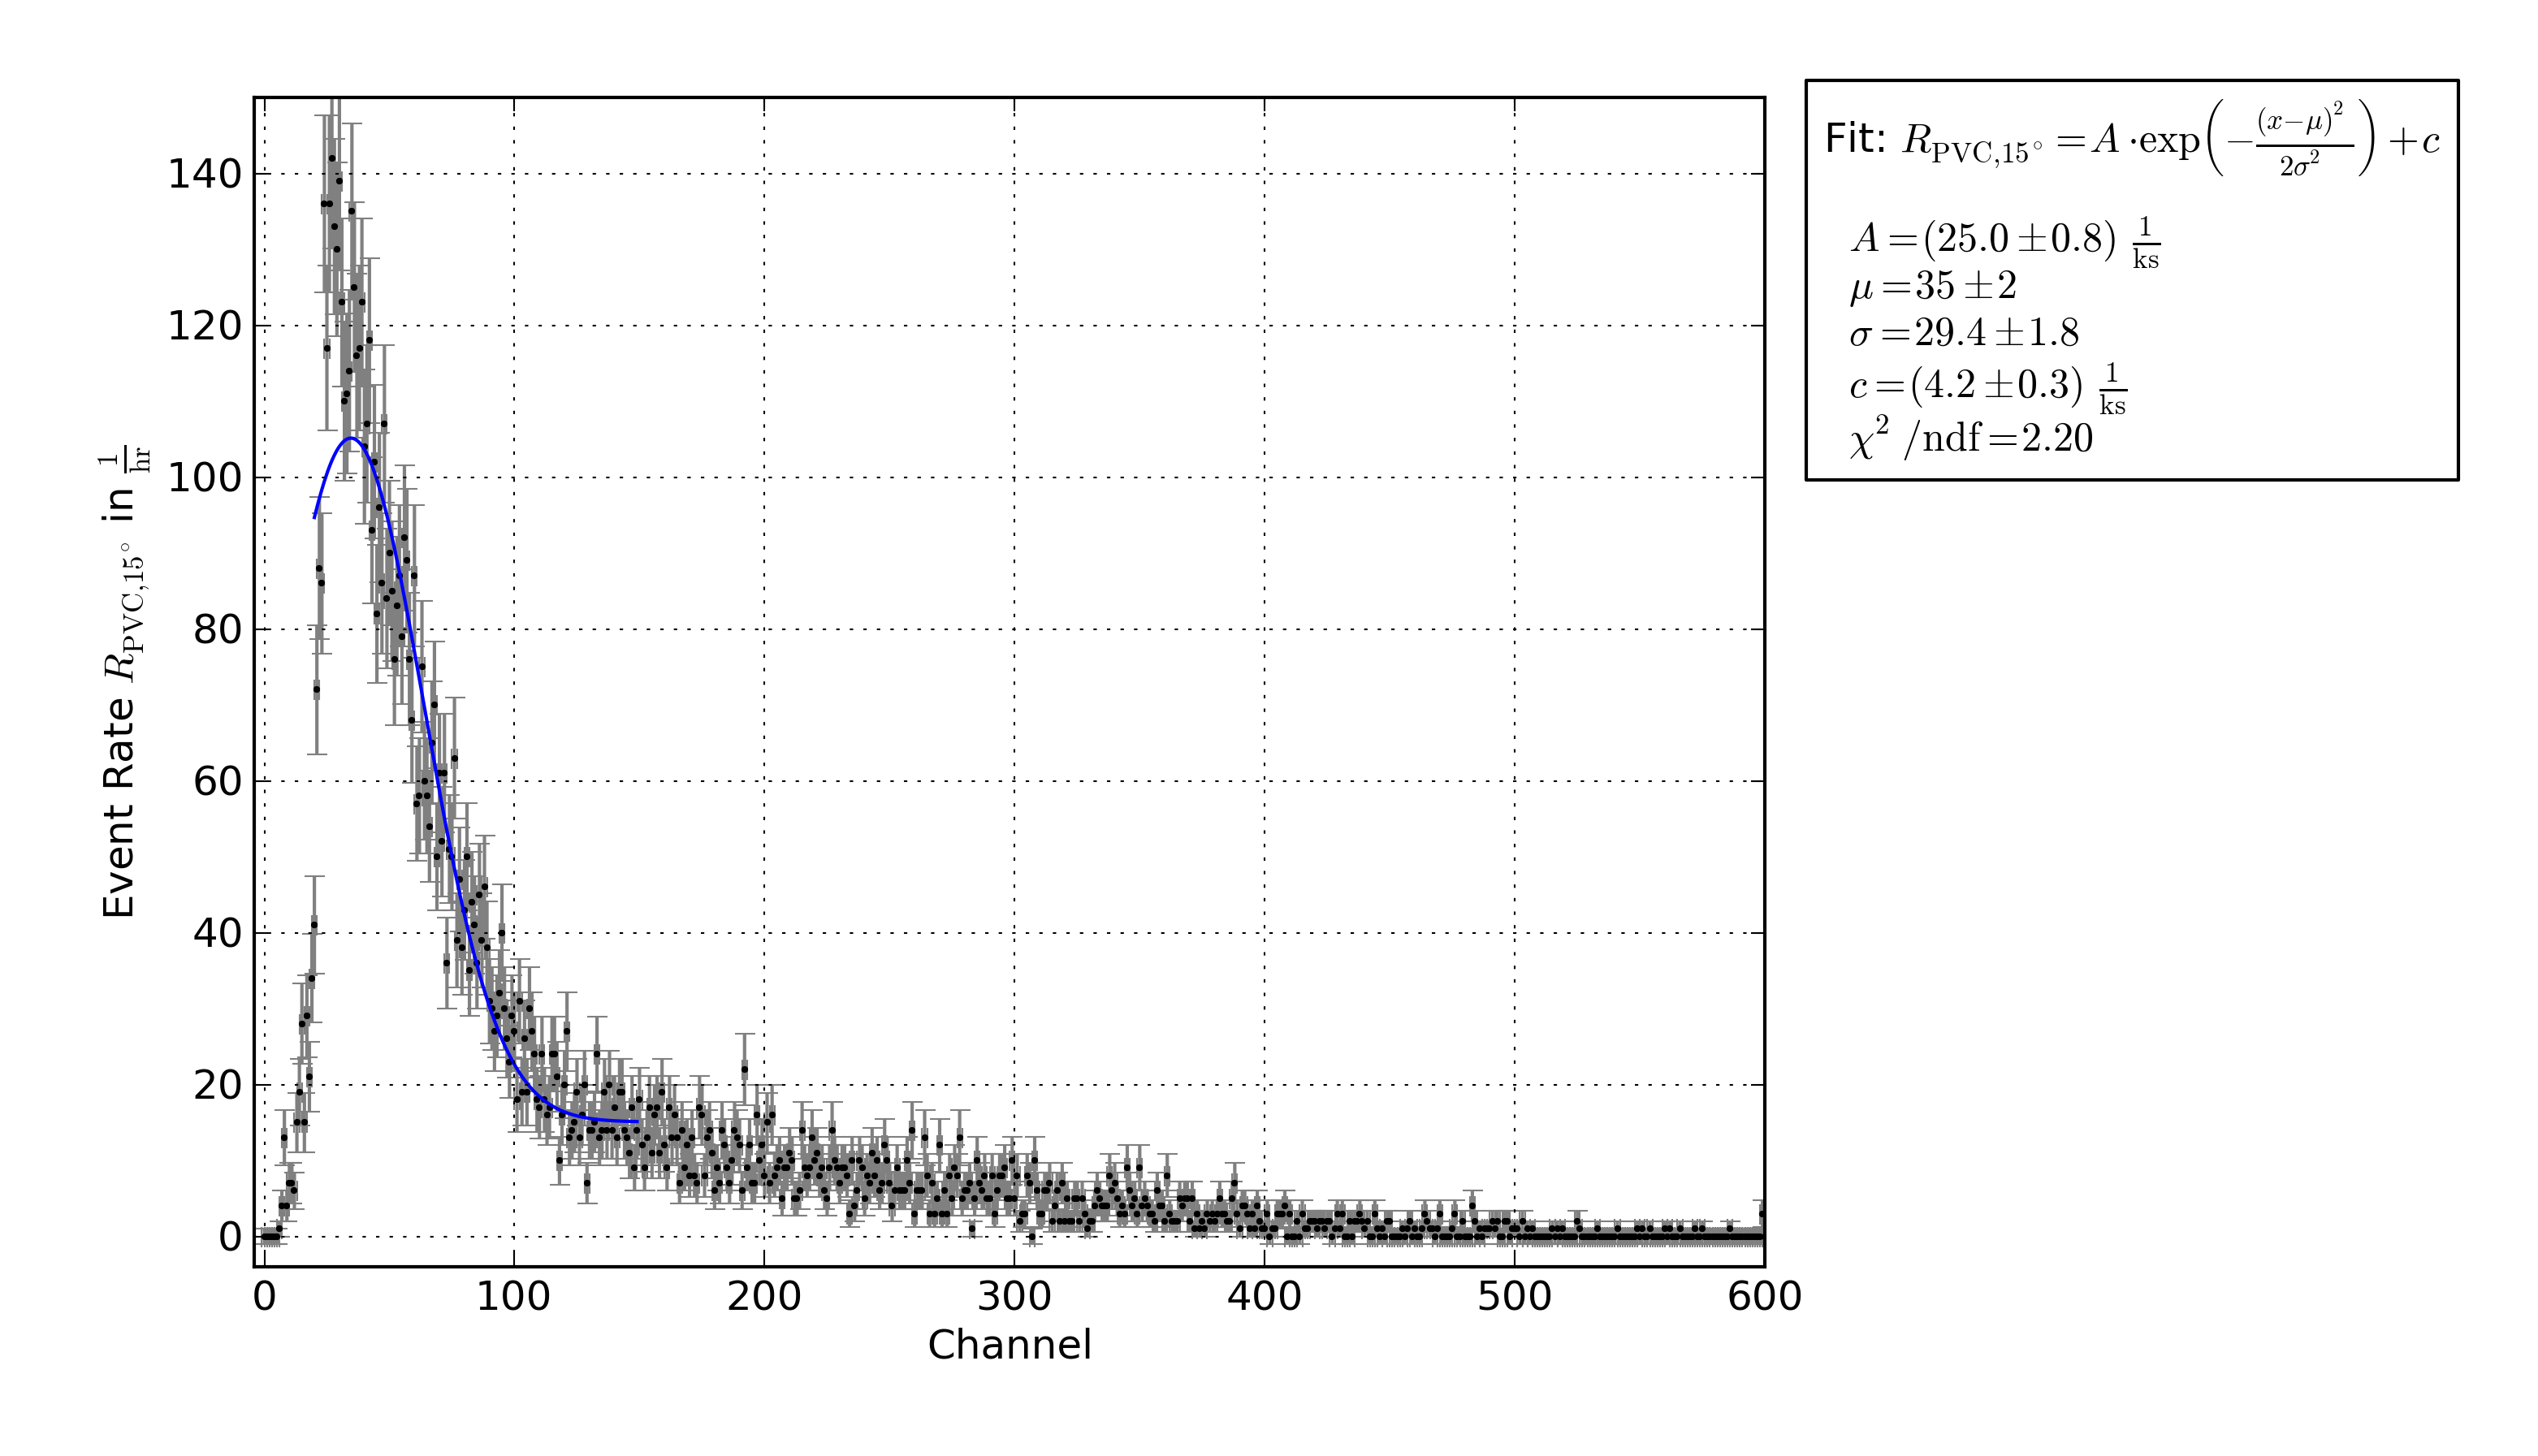
\includegraphics[width=0.6\textwidth]{plots/pvc_15.png}
  \caption{Electron energy spectrum (PVC scintillator) of coincident signals
  with $\theta=15\degree$. Measurement duration $t=3600\mathrm{s}$.}
  \label{fig:pvc15}
\end{figure}
\begin{figure}[h!]
  \centering
  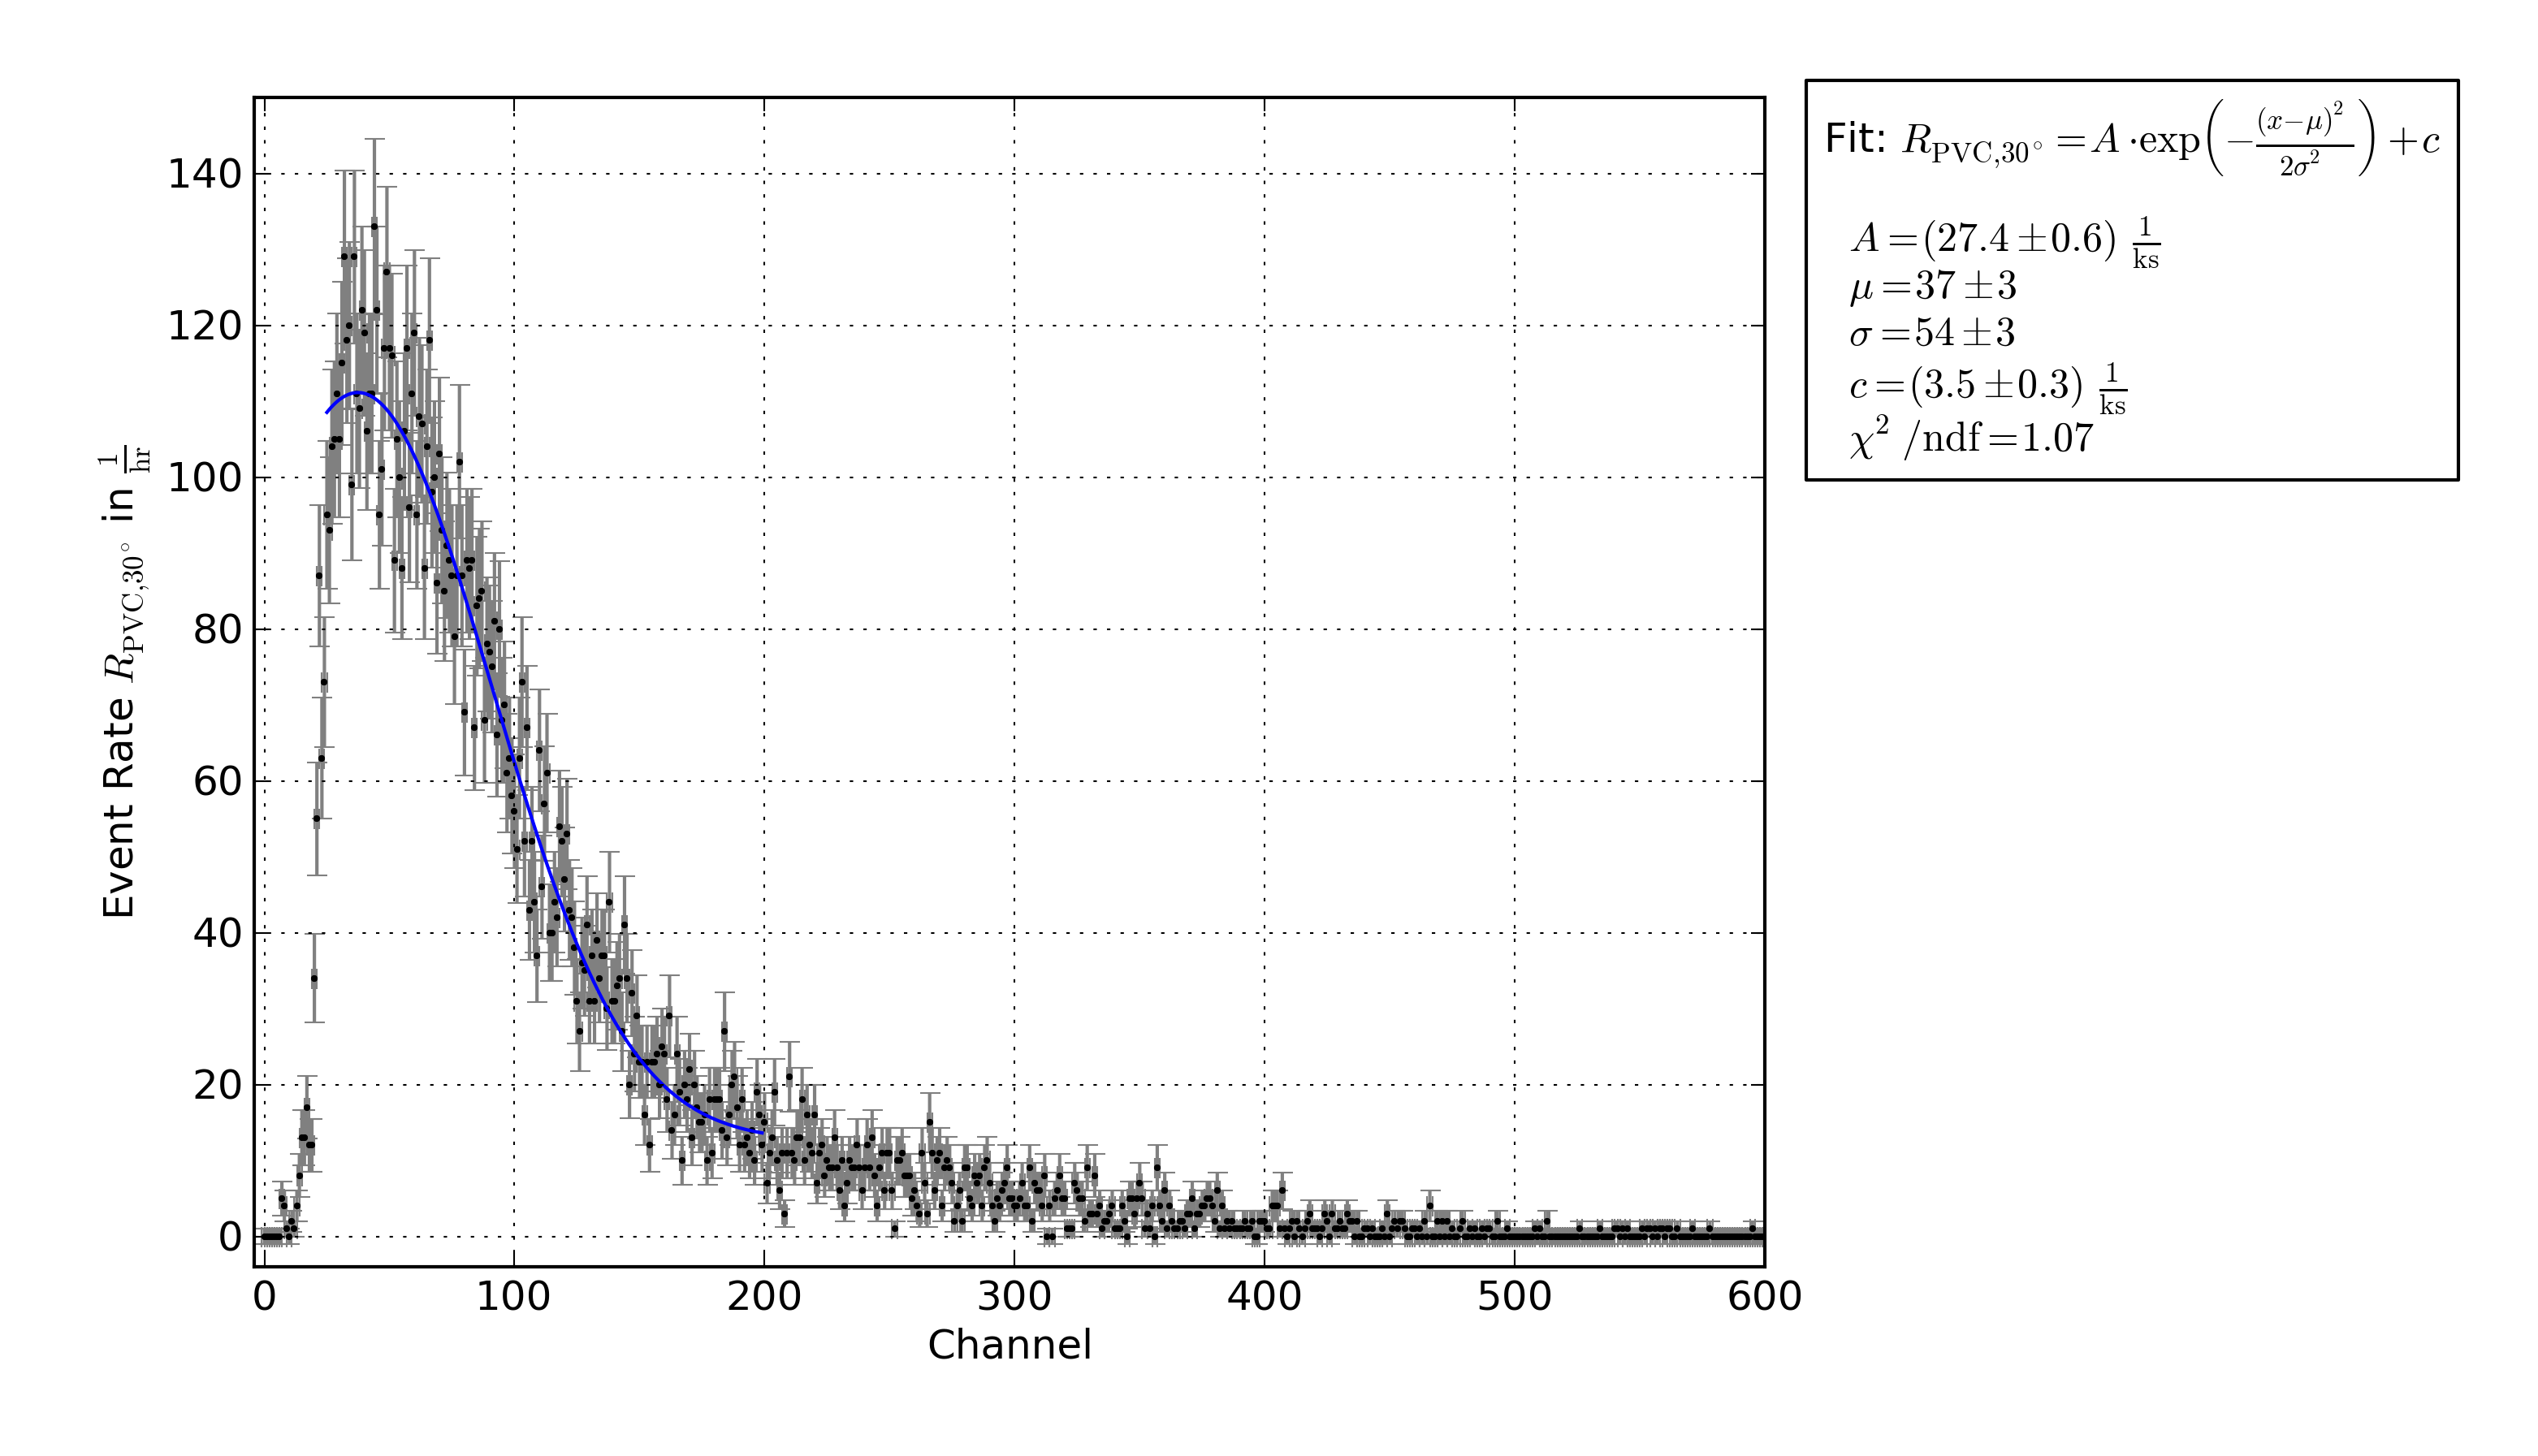
\includegraphics[width=0.6\textwidth]{plots/pvc_30.png}
  \caption{Electron energy spectrum (PVC scintillator) of coincident signals
  with $\theta=30\degree$. Measurement duration $t=3699.34{s}$.}
  \label{fig:pvc30}
\end{figure}
\begin{figure}[h!]
  \centering
  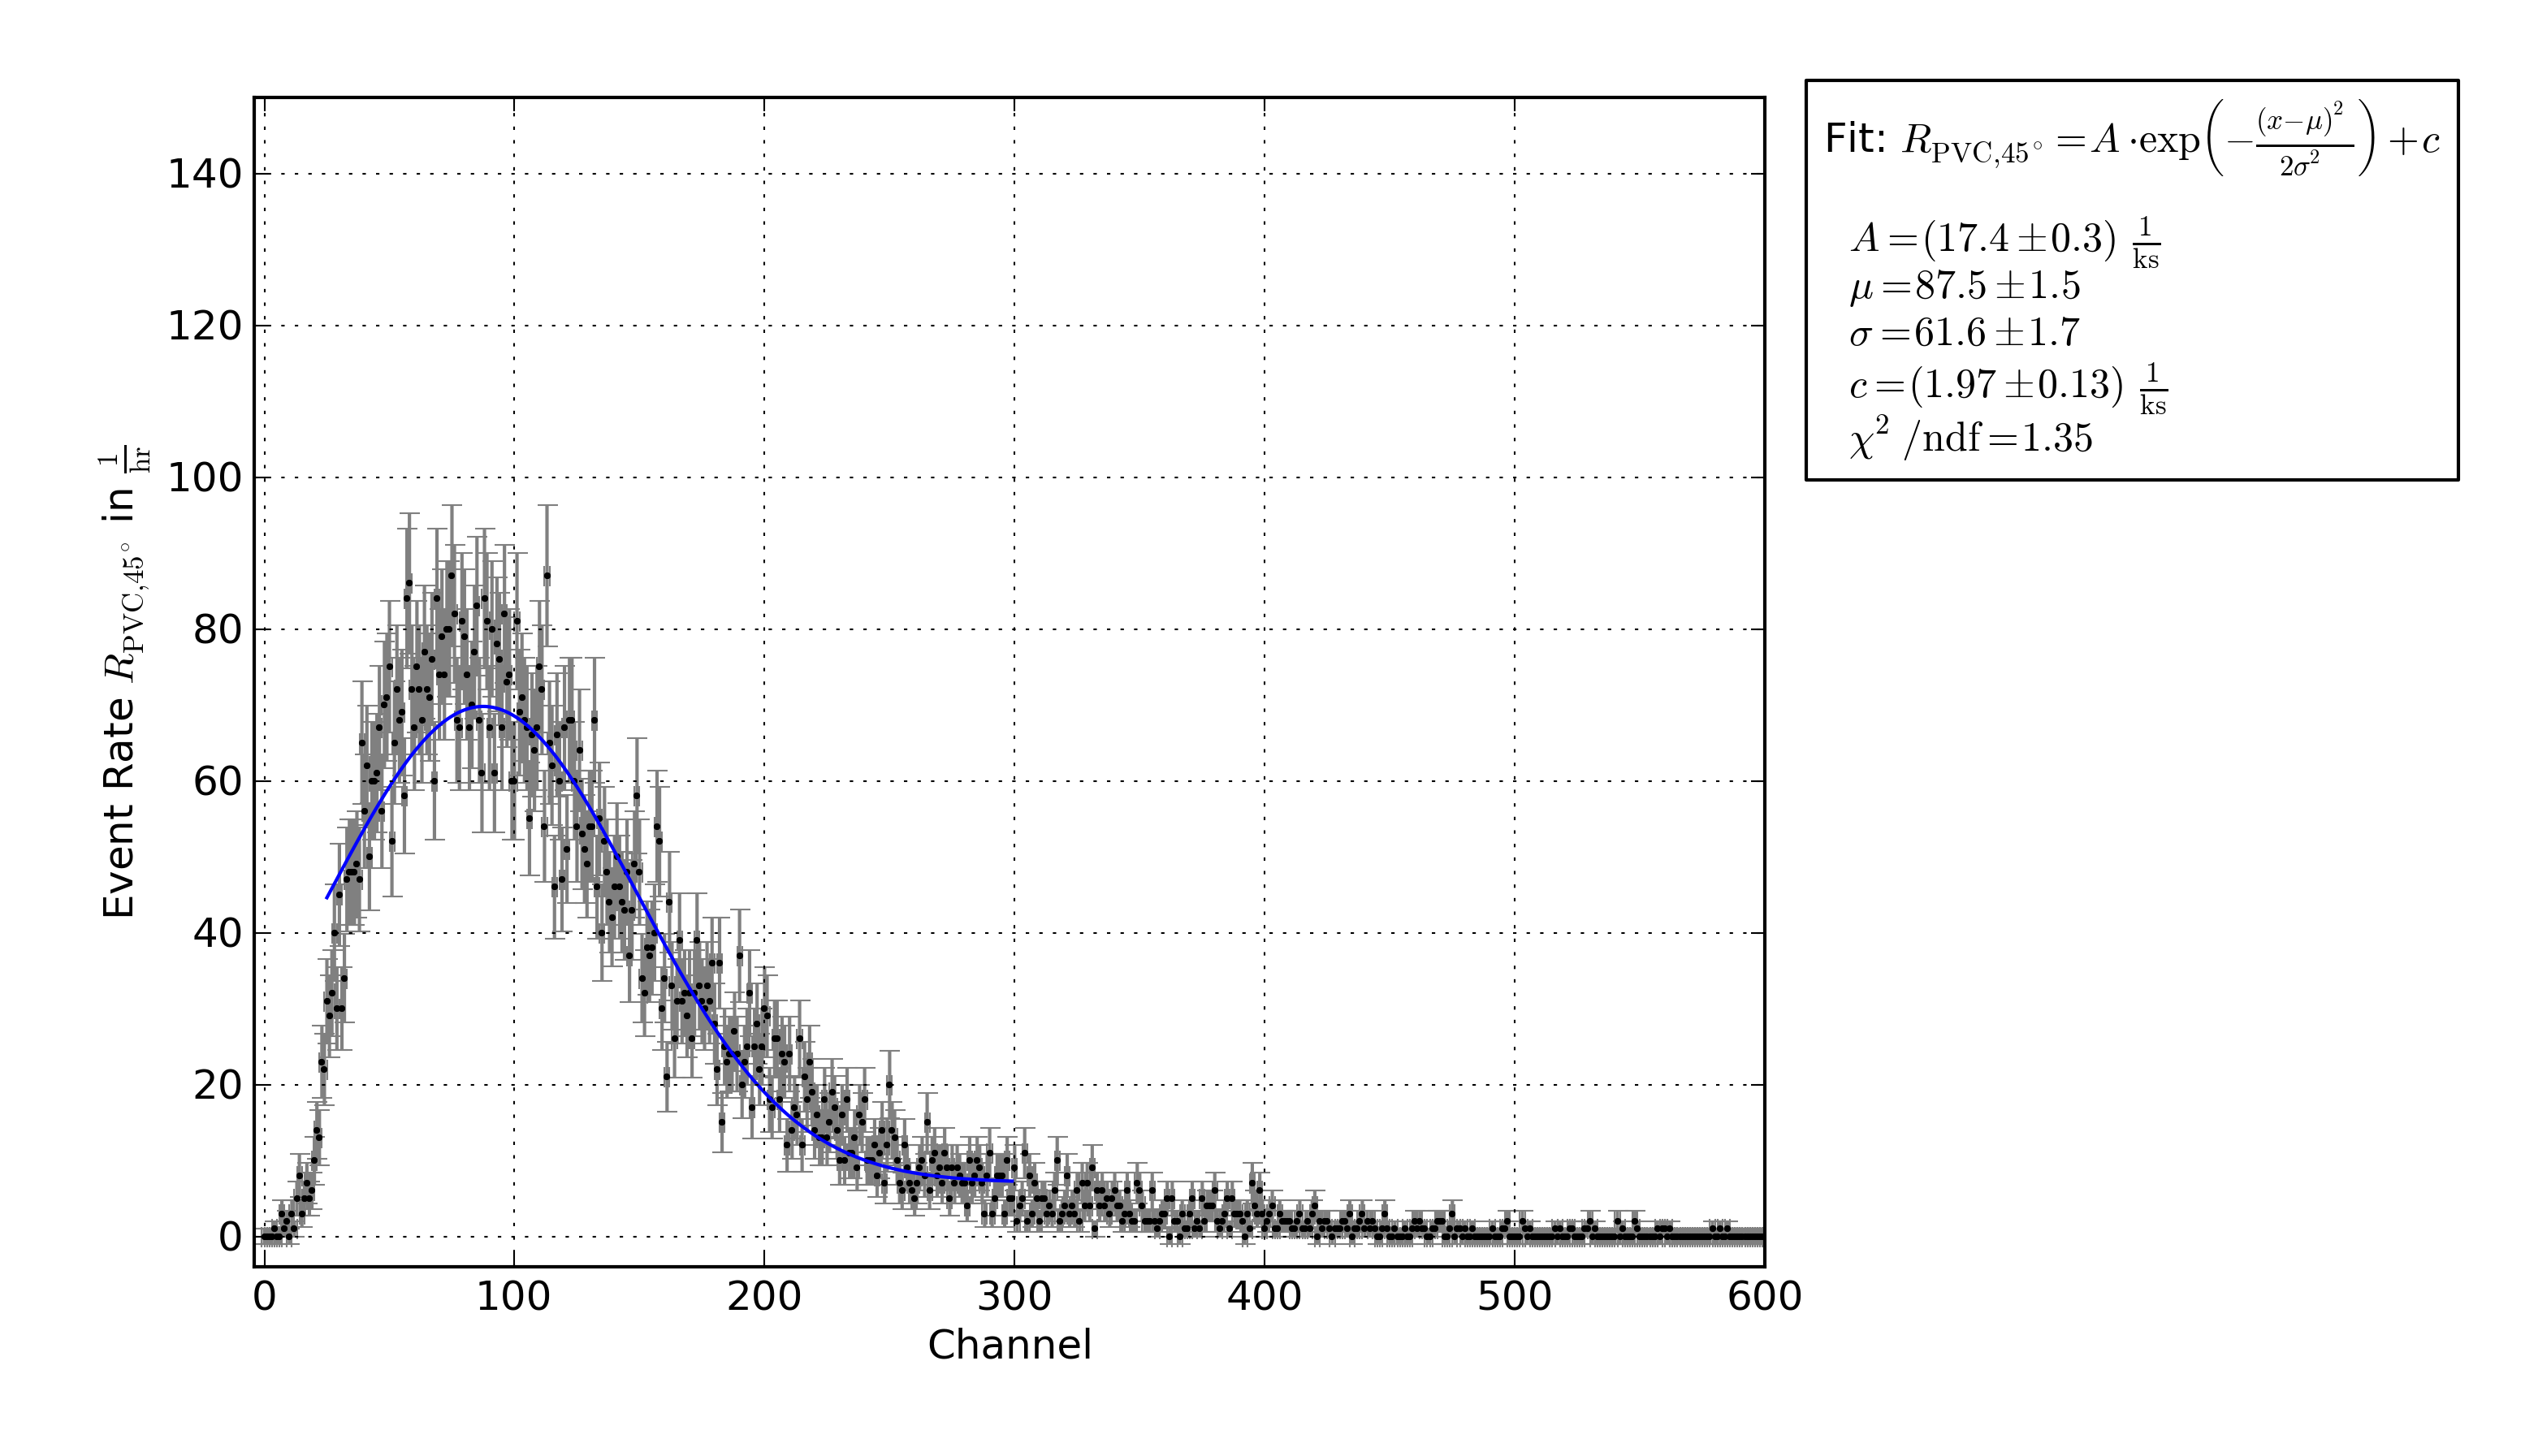
\includegraphics[width=0.6\textwidth]{plots/pvc_45.png}
  \caption{Electron energy spectrum (PVC scintillator) of coincident signals
  with $\theta=45\degree$. Measurement duration $t=3600\mathrm{s}$.}
  \label{fig:pvc45}
\end{figure}
\begin{figure}[h!]
  \centering
  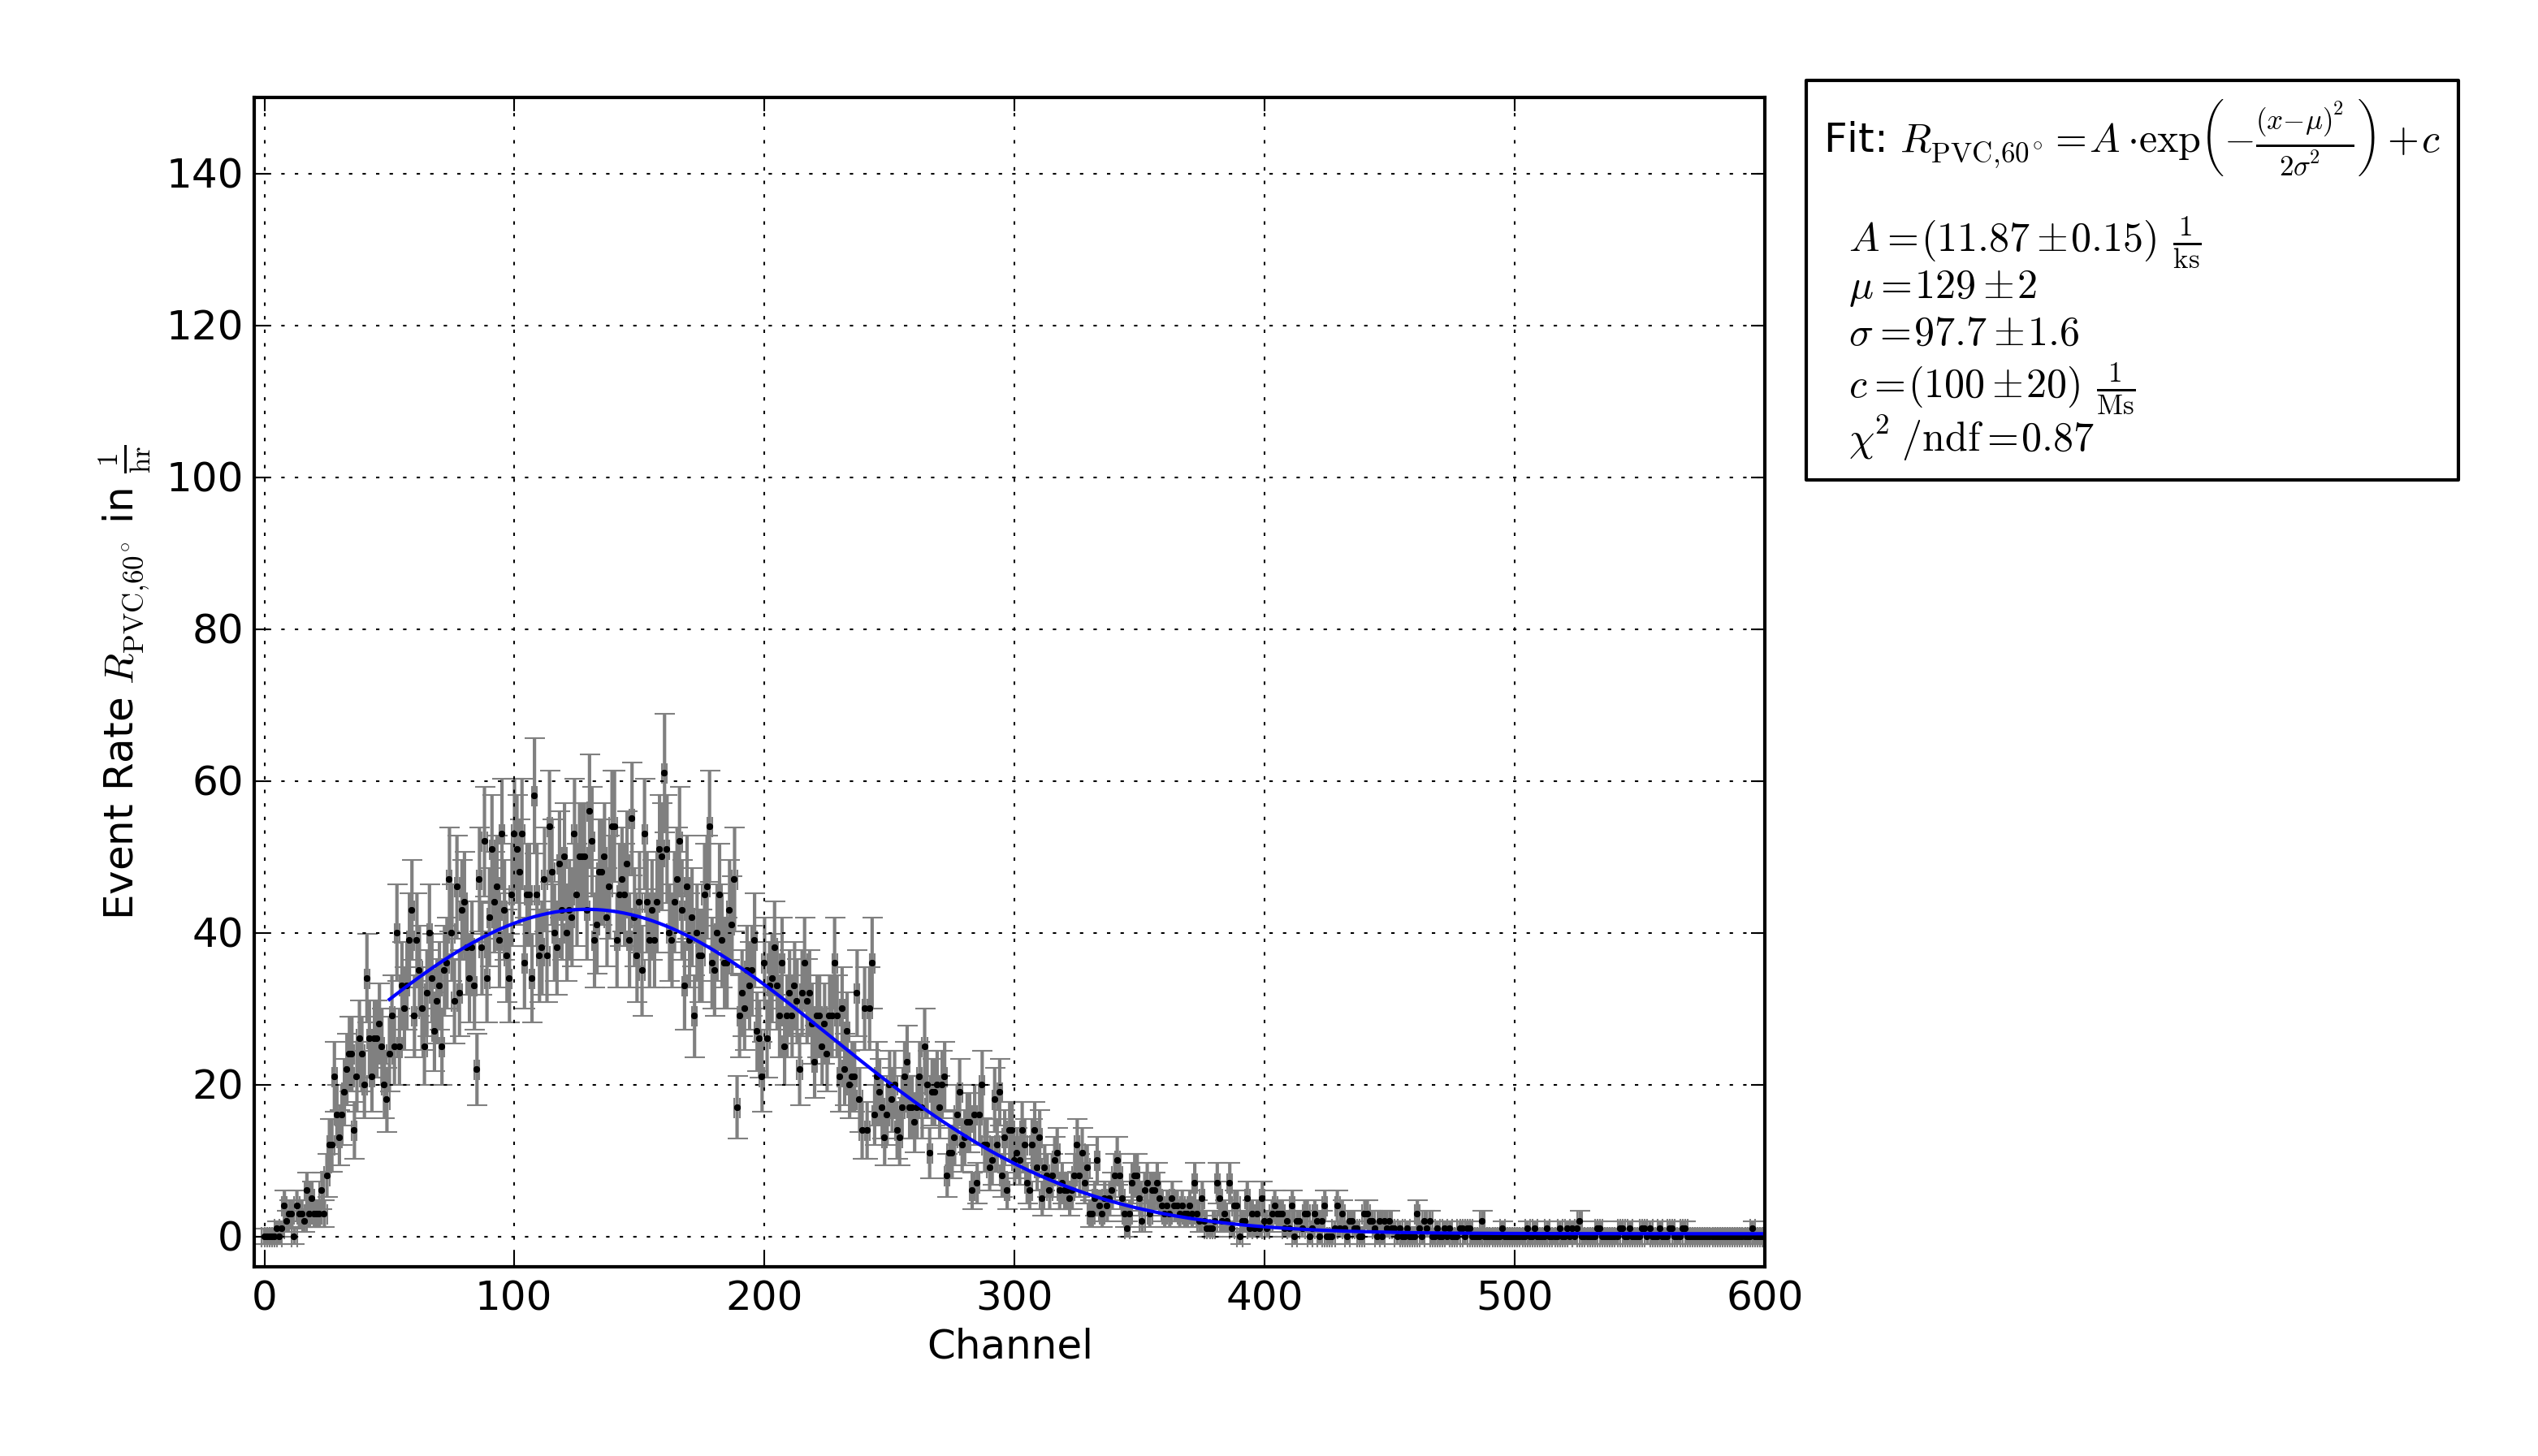
\includegraphics[width=0.6\textwidth]{plots/pvc_60.png}
  \caption{Electron energy spectrum (PVC scintillator) of coincident signals
  with $\theta=60\degree$. Measurement duration $t=3600\mathrm{s}$.}
  \label{fig:pvc60}
\end{figure}
\begin{figure}[h!]
  \centering
  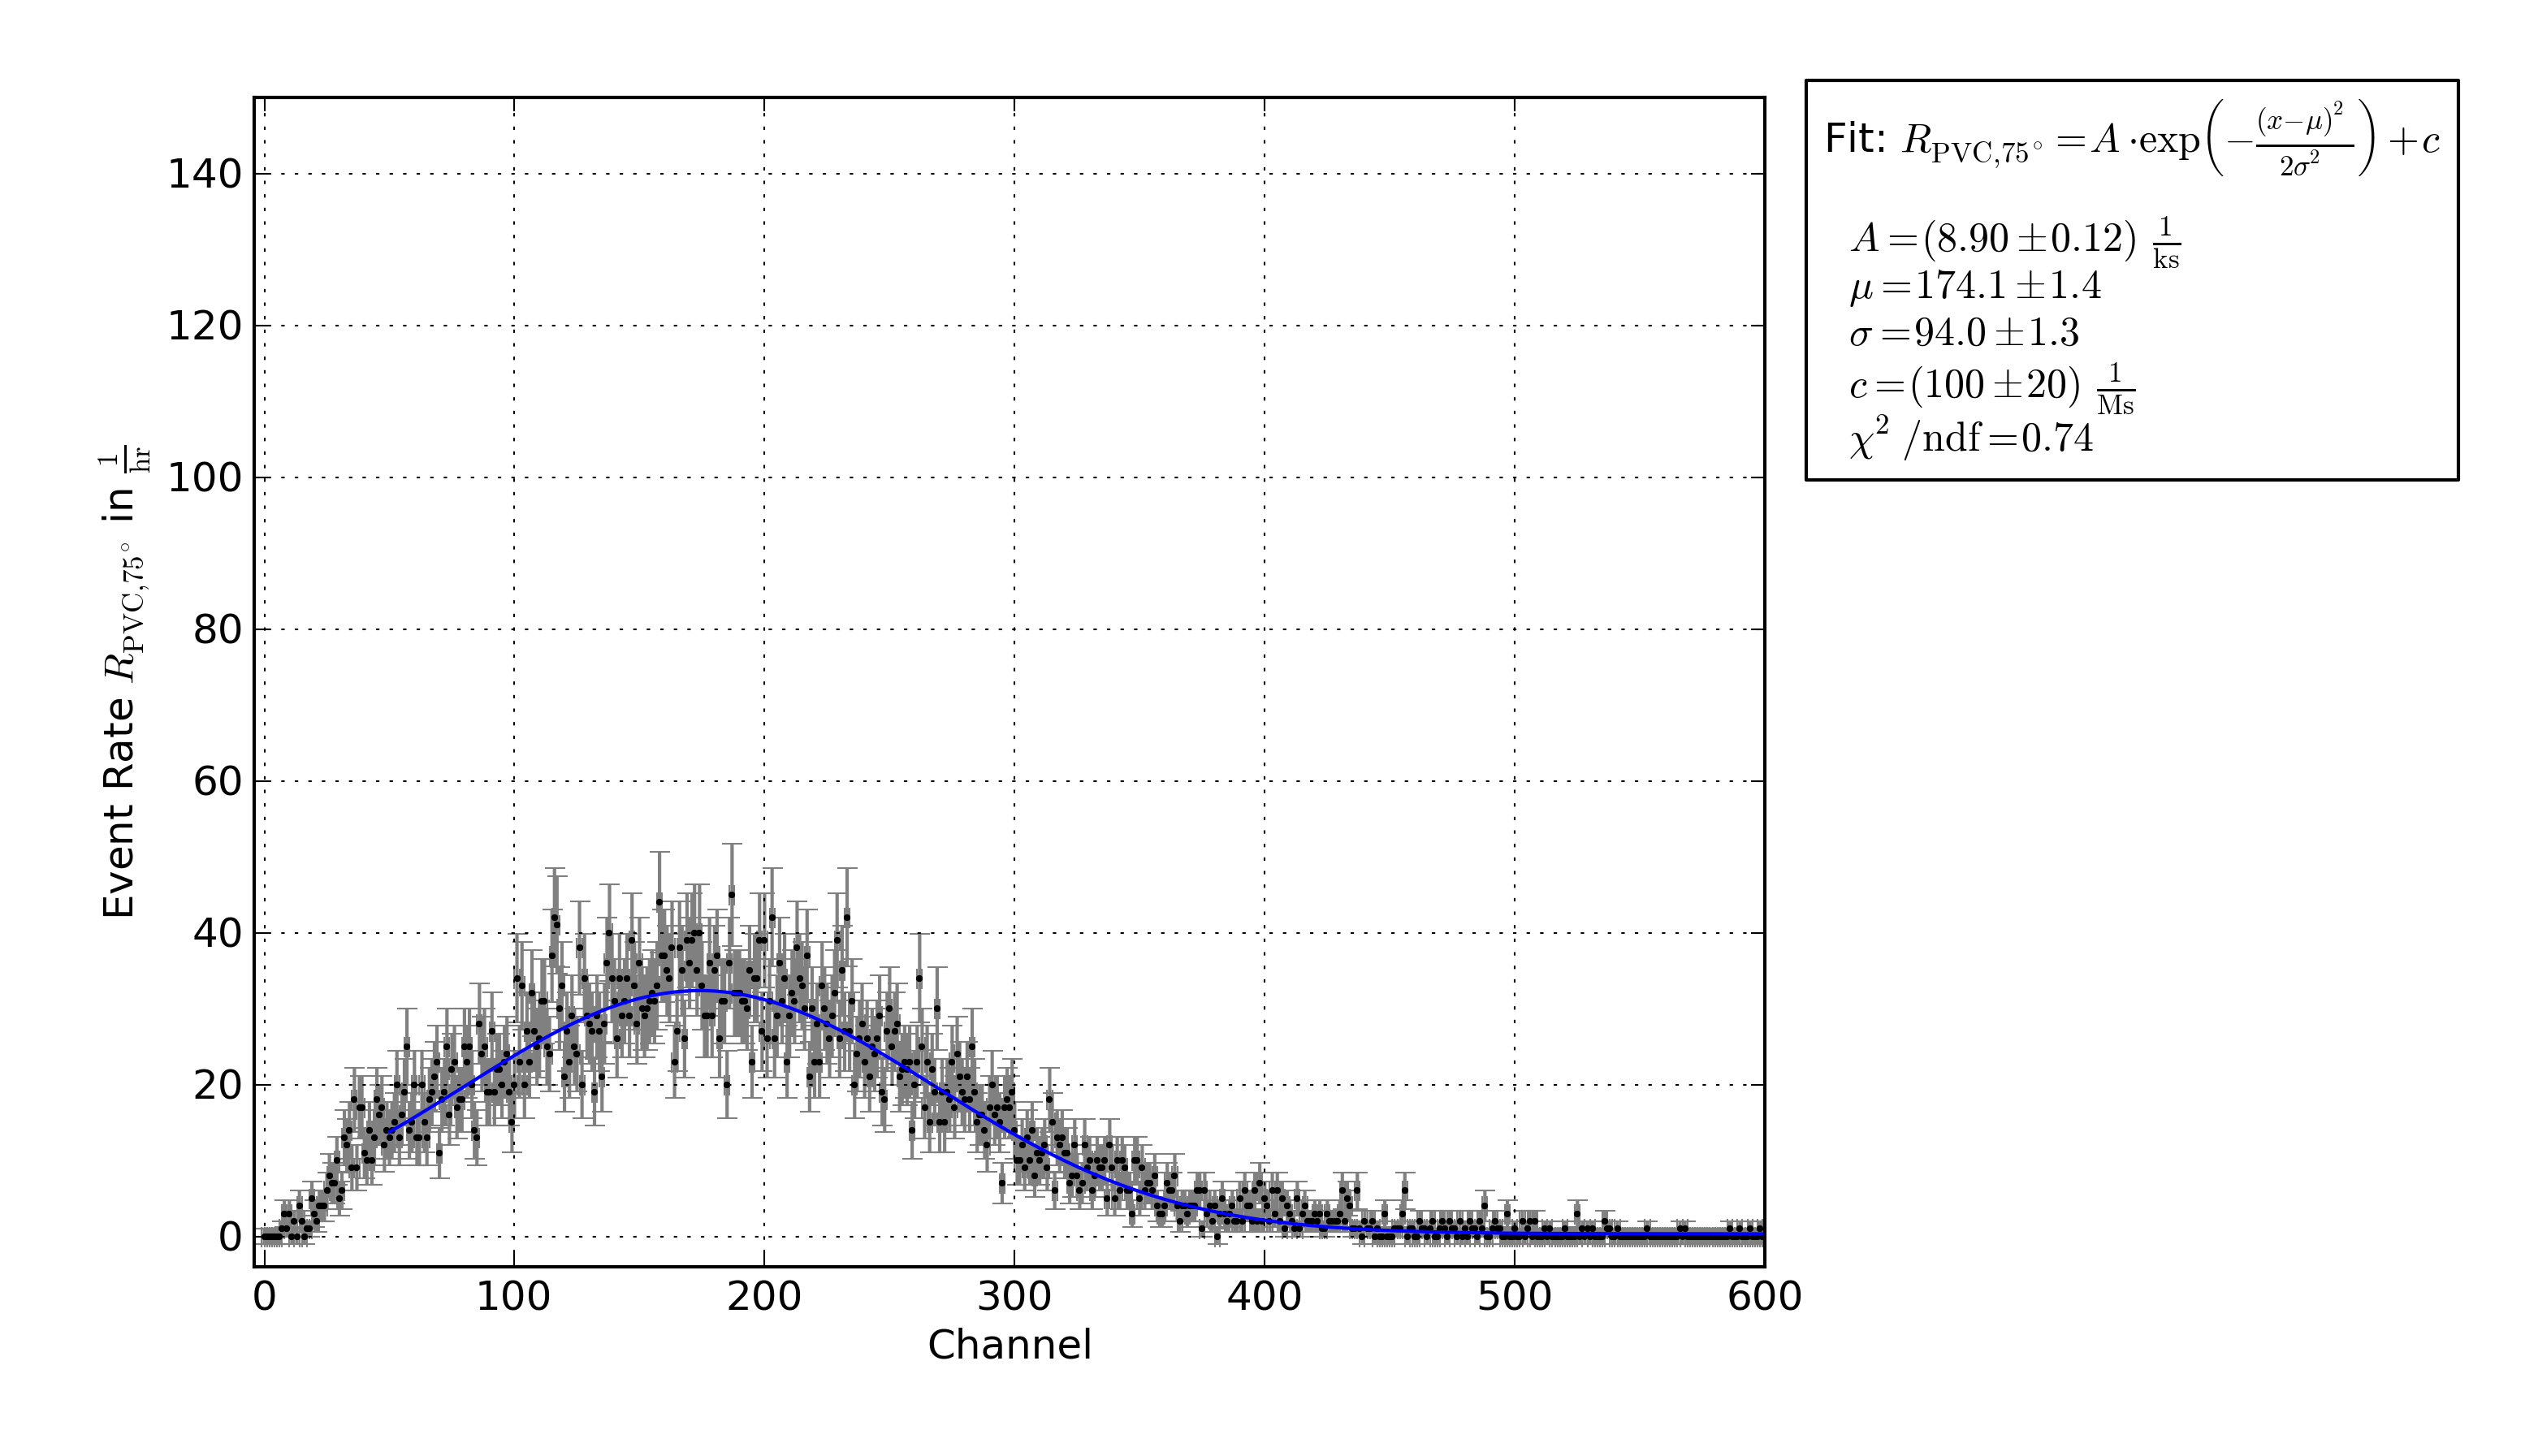
\includegraphics[width=0.6\textwidth]{plots/pvc_75.png}
  \caption{Electron energy spectrum (PVC scintillator) of coincident signals
  with $\theta=75\degree$. Measurement duration $t=3600\mathrm{s}$.}
  \label{fig:pvc75}
\end{figure}
\begin{figure}[h!]
  \centering
  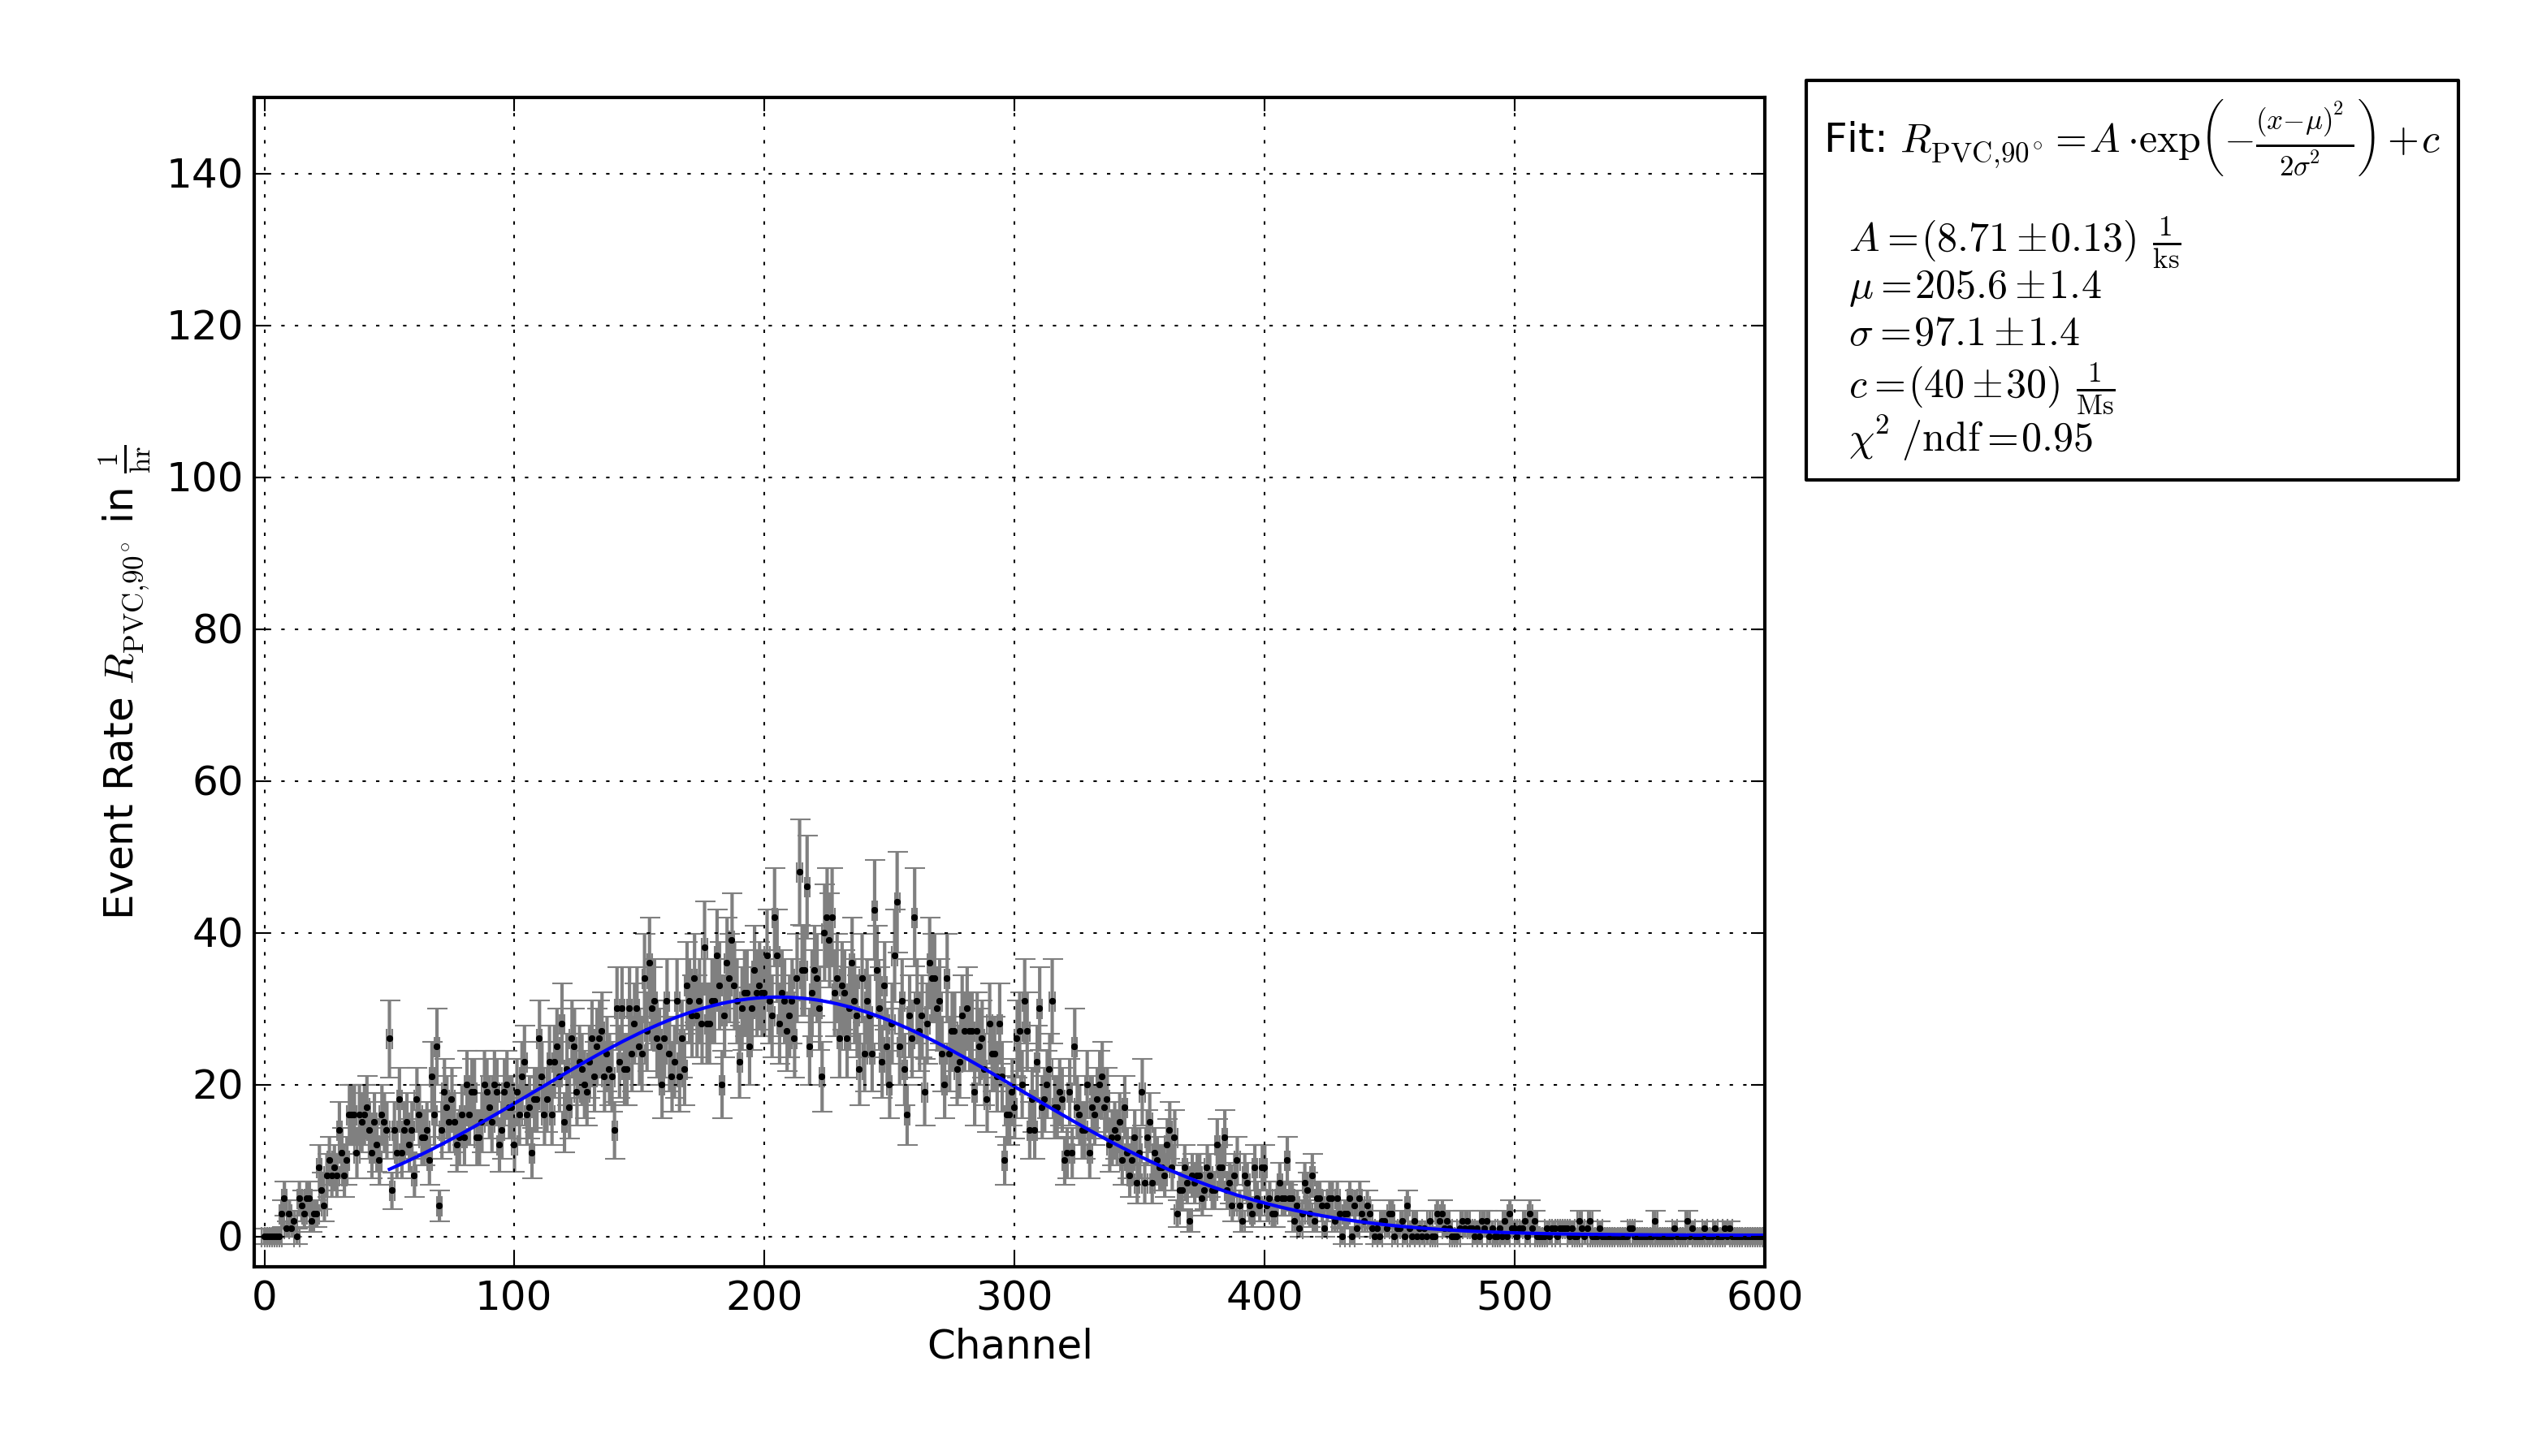
\includegraphics[width=0.6\textwidth]{plots/pvc_90.png}
  \caption{Electron energy spectrum (PVC scintillator) of coincident signals
  with $\theta=90\degree$. Measurement duration $t=3600\mathrm{s}$.}
  \label{fig:pvc90}
\end{figure}
\begin{figure}[h!]
  \centering
  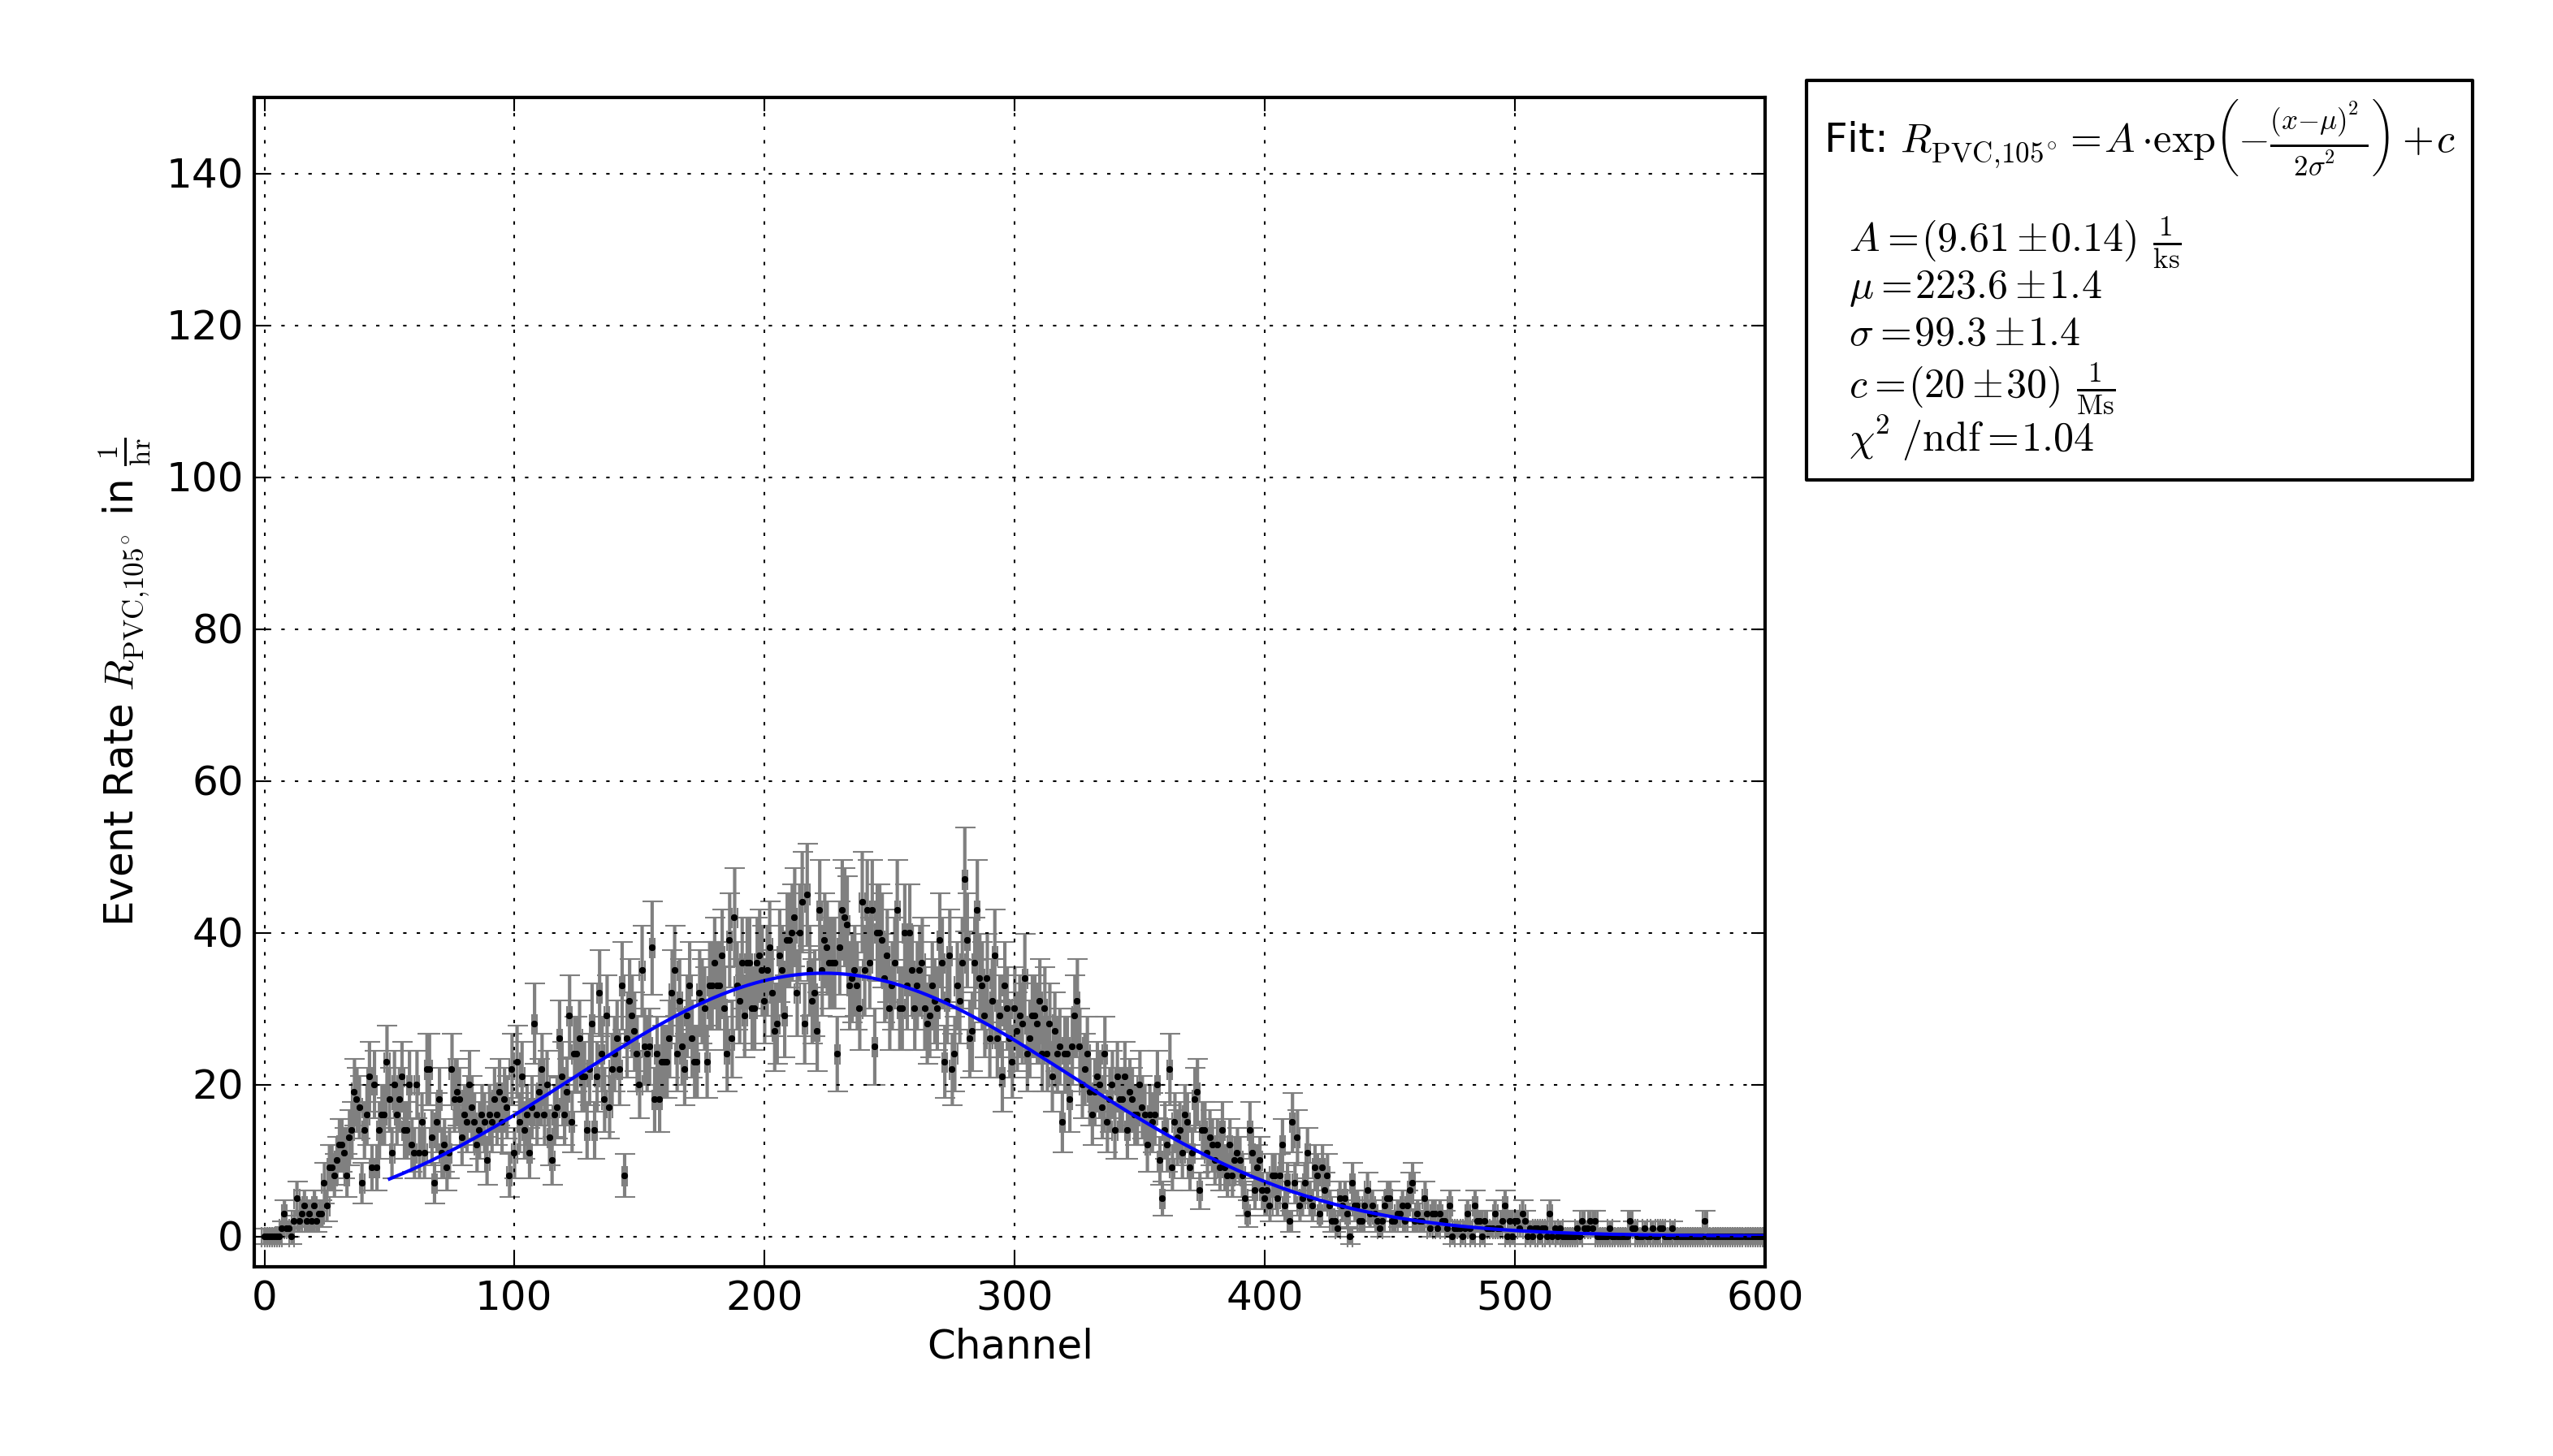
\includegraphics[width=0.6\textwidth]{plots/pvc_105.png}
  \caption{Electron energy spectrum (PVC scintillator) of coincident signals
  with $\theta=105\degree$. Measurement duration $t=3600\mathrm{s}$.}
  \label{fig:pvc105}
\end{figure}
\begin{figure}[h!]
  \centering
  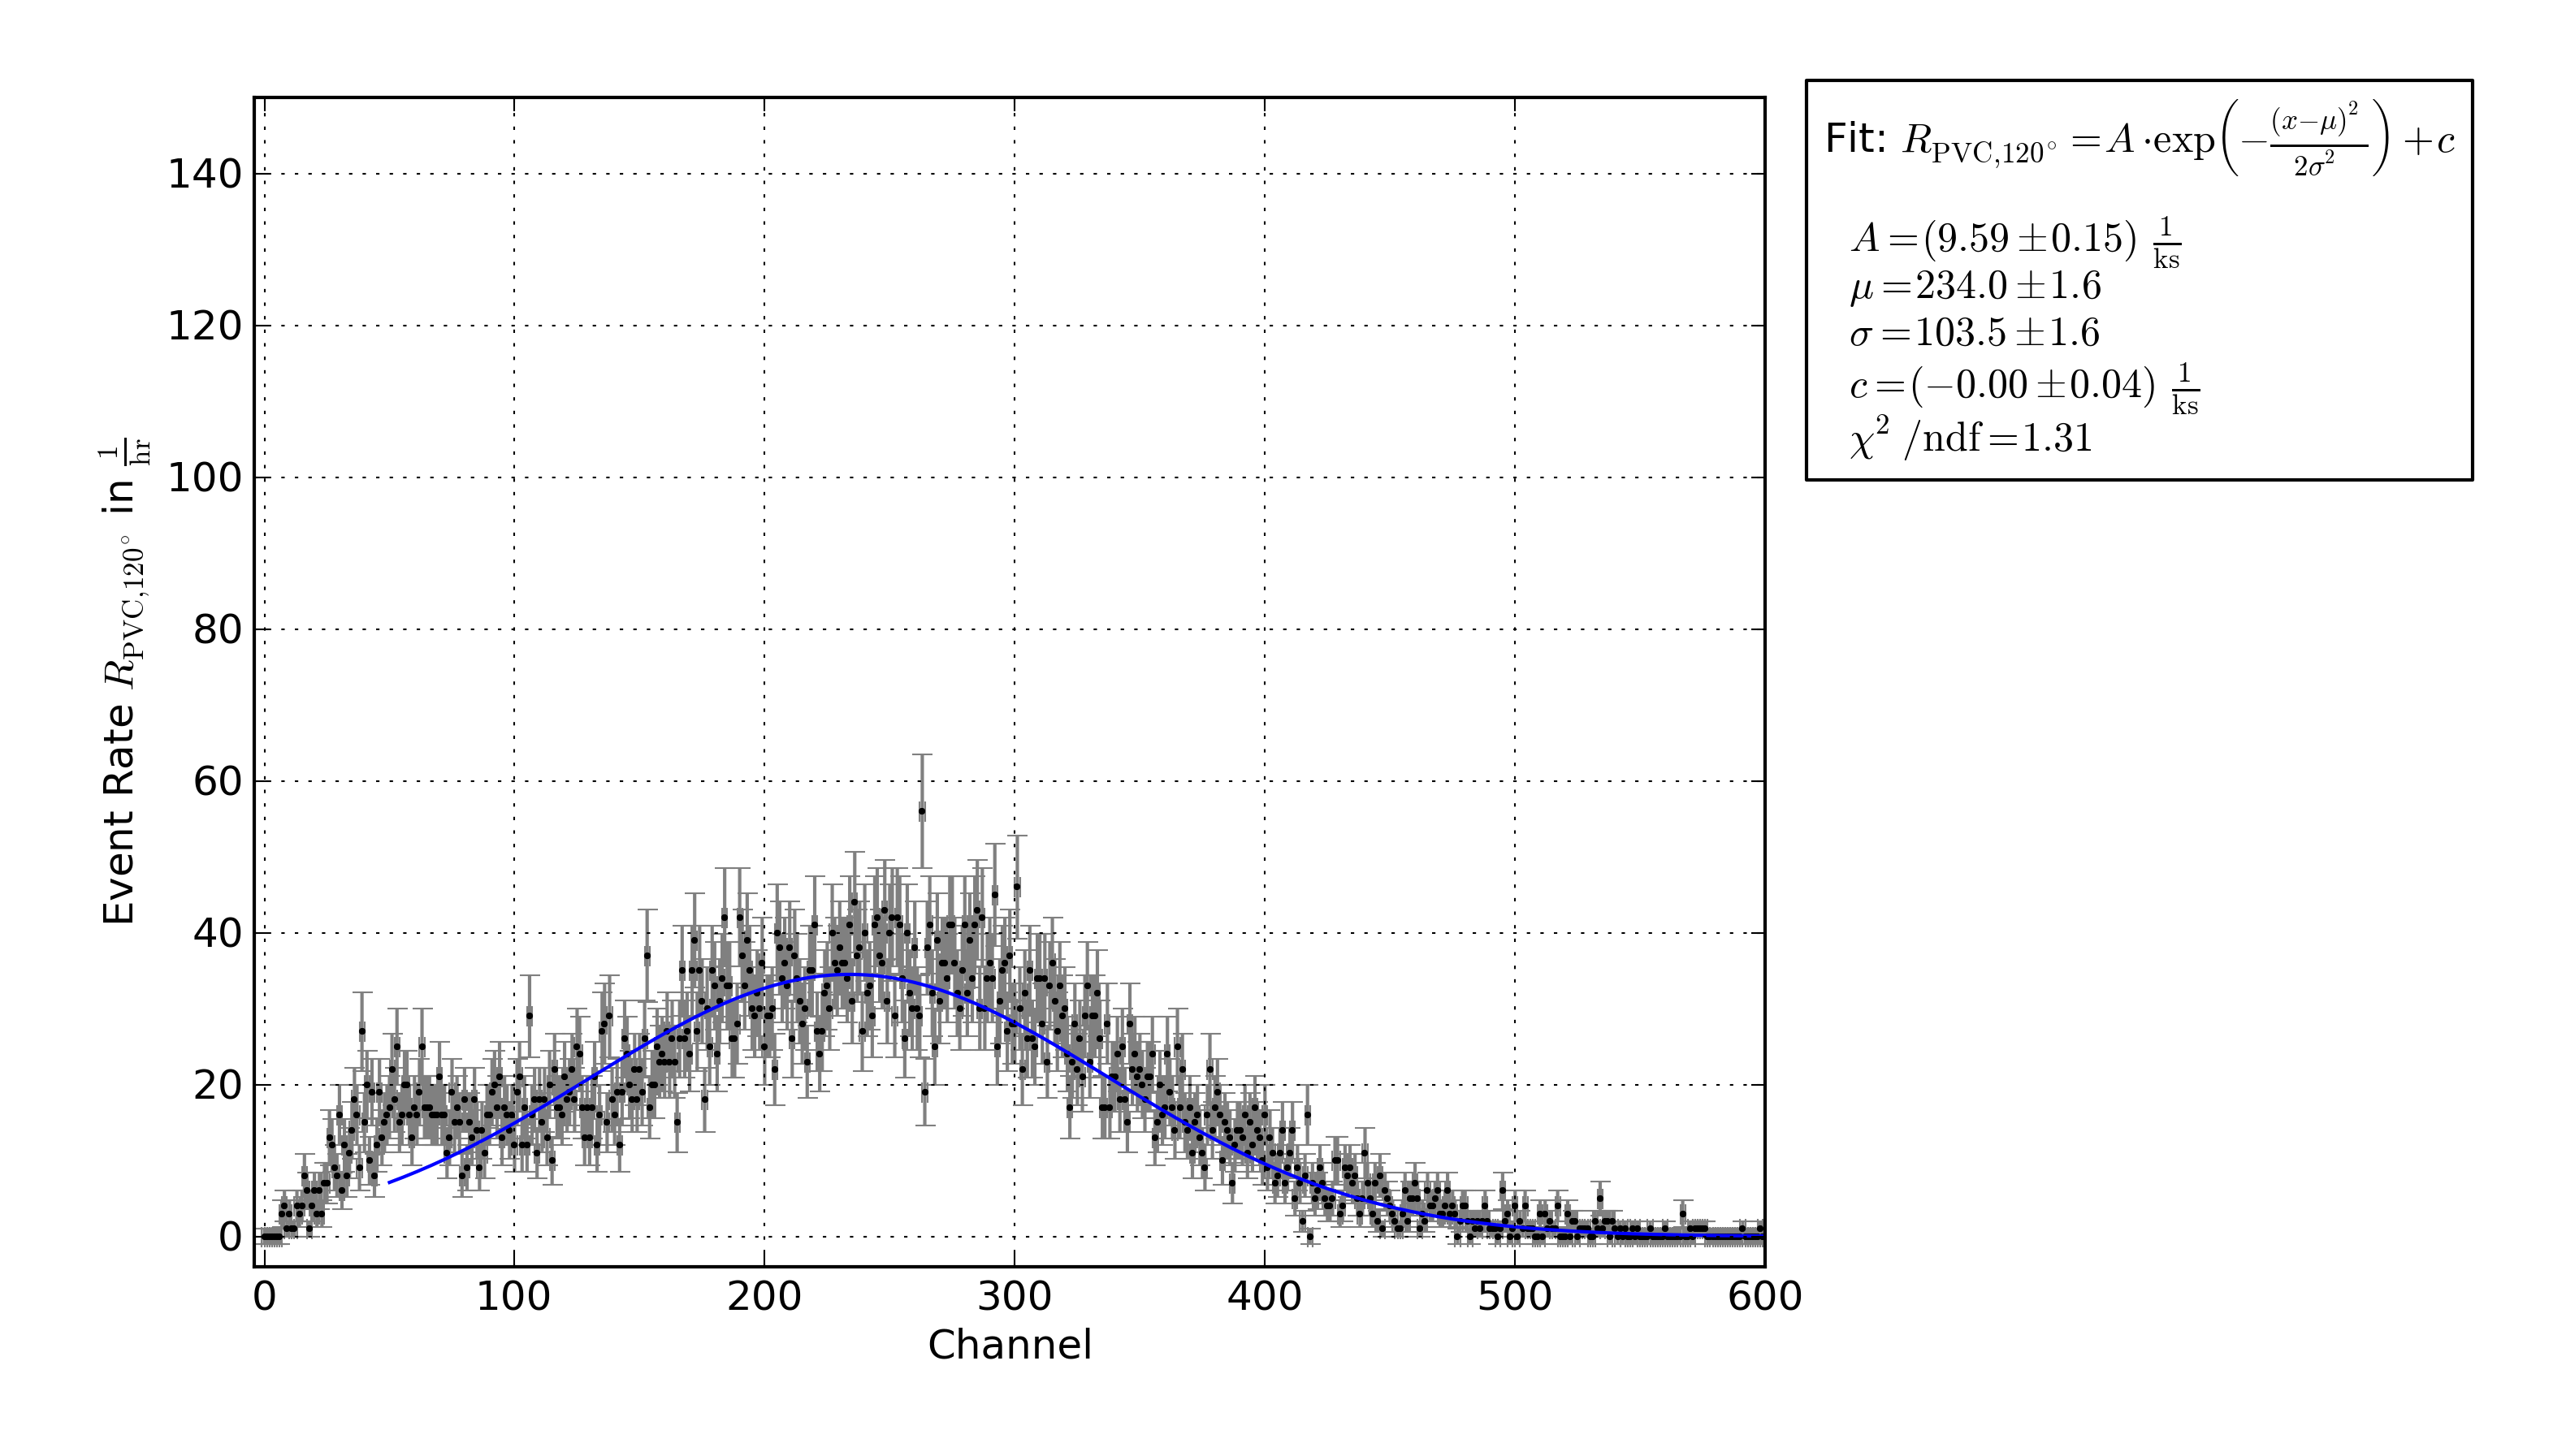
\includegraphics[width=0.6\textwidth]{plots/pvc_120.png}
  \caption{Electron energy spectrum (PVC scintillator) of coincident signals
  with $\theta=120\degree$. Measurement duration $t=3600\mathrm{s}$.}
  \label{fig:pvc120}
\end{figure}

\FloatBarrier
\subsubsection{Anorganic Scintillator}
\begin{figure}[h!]
  \centering
  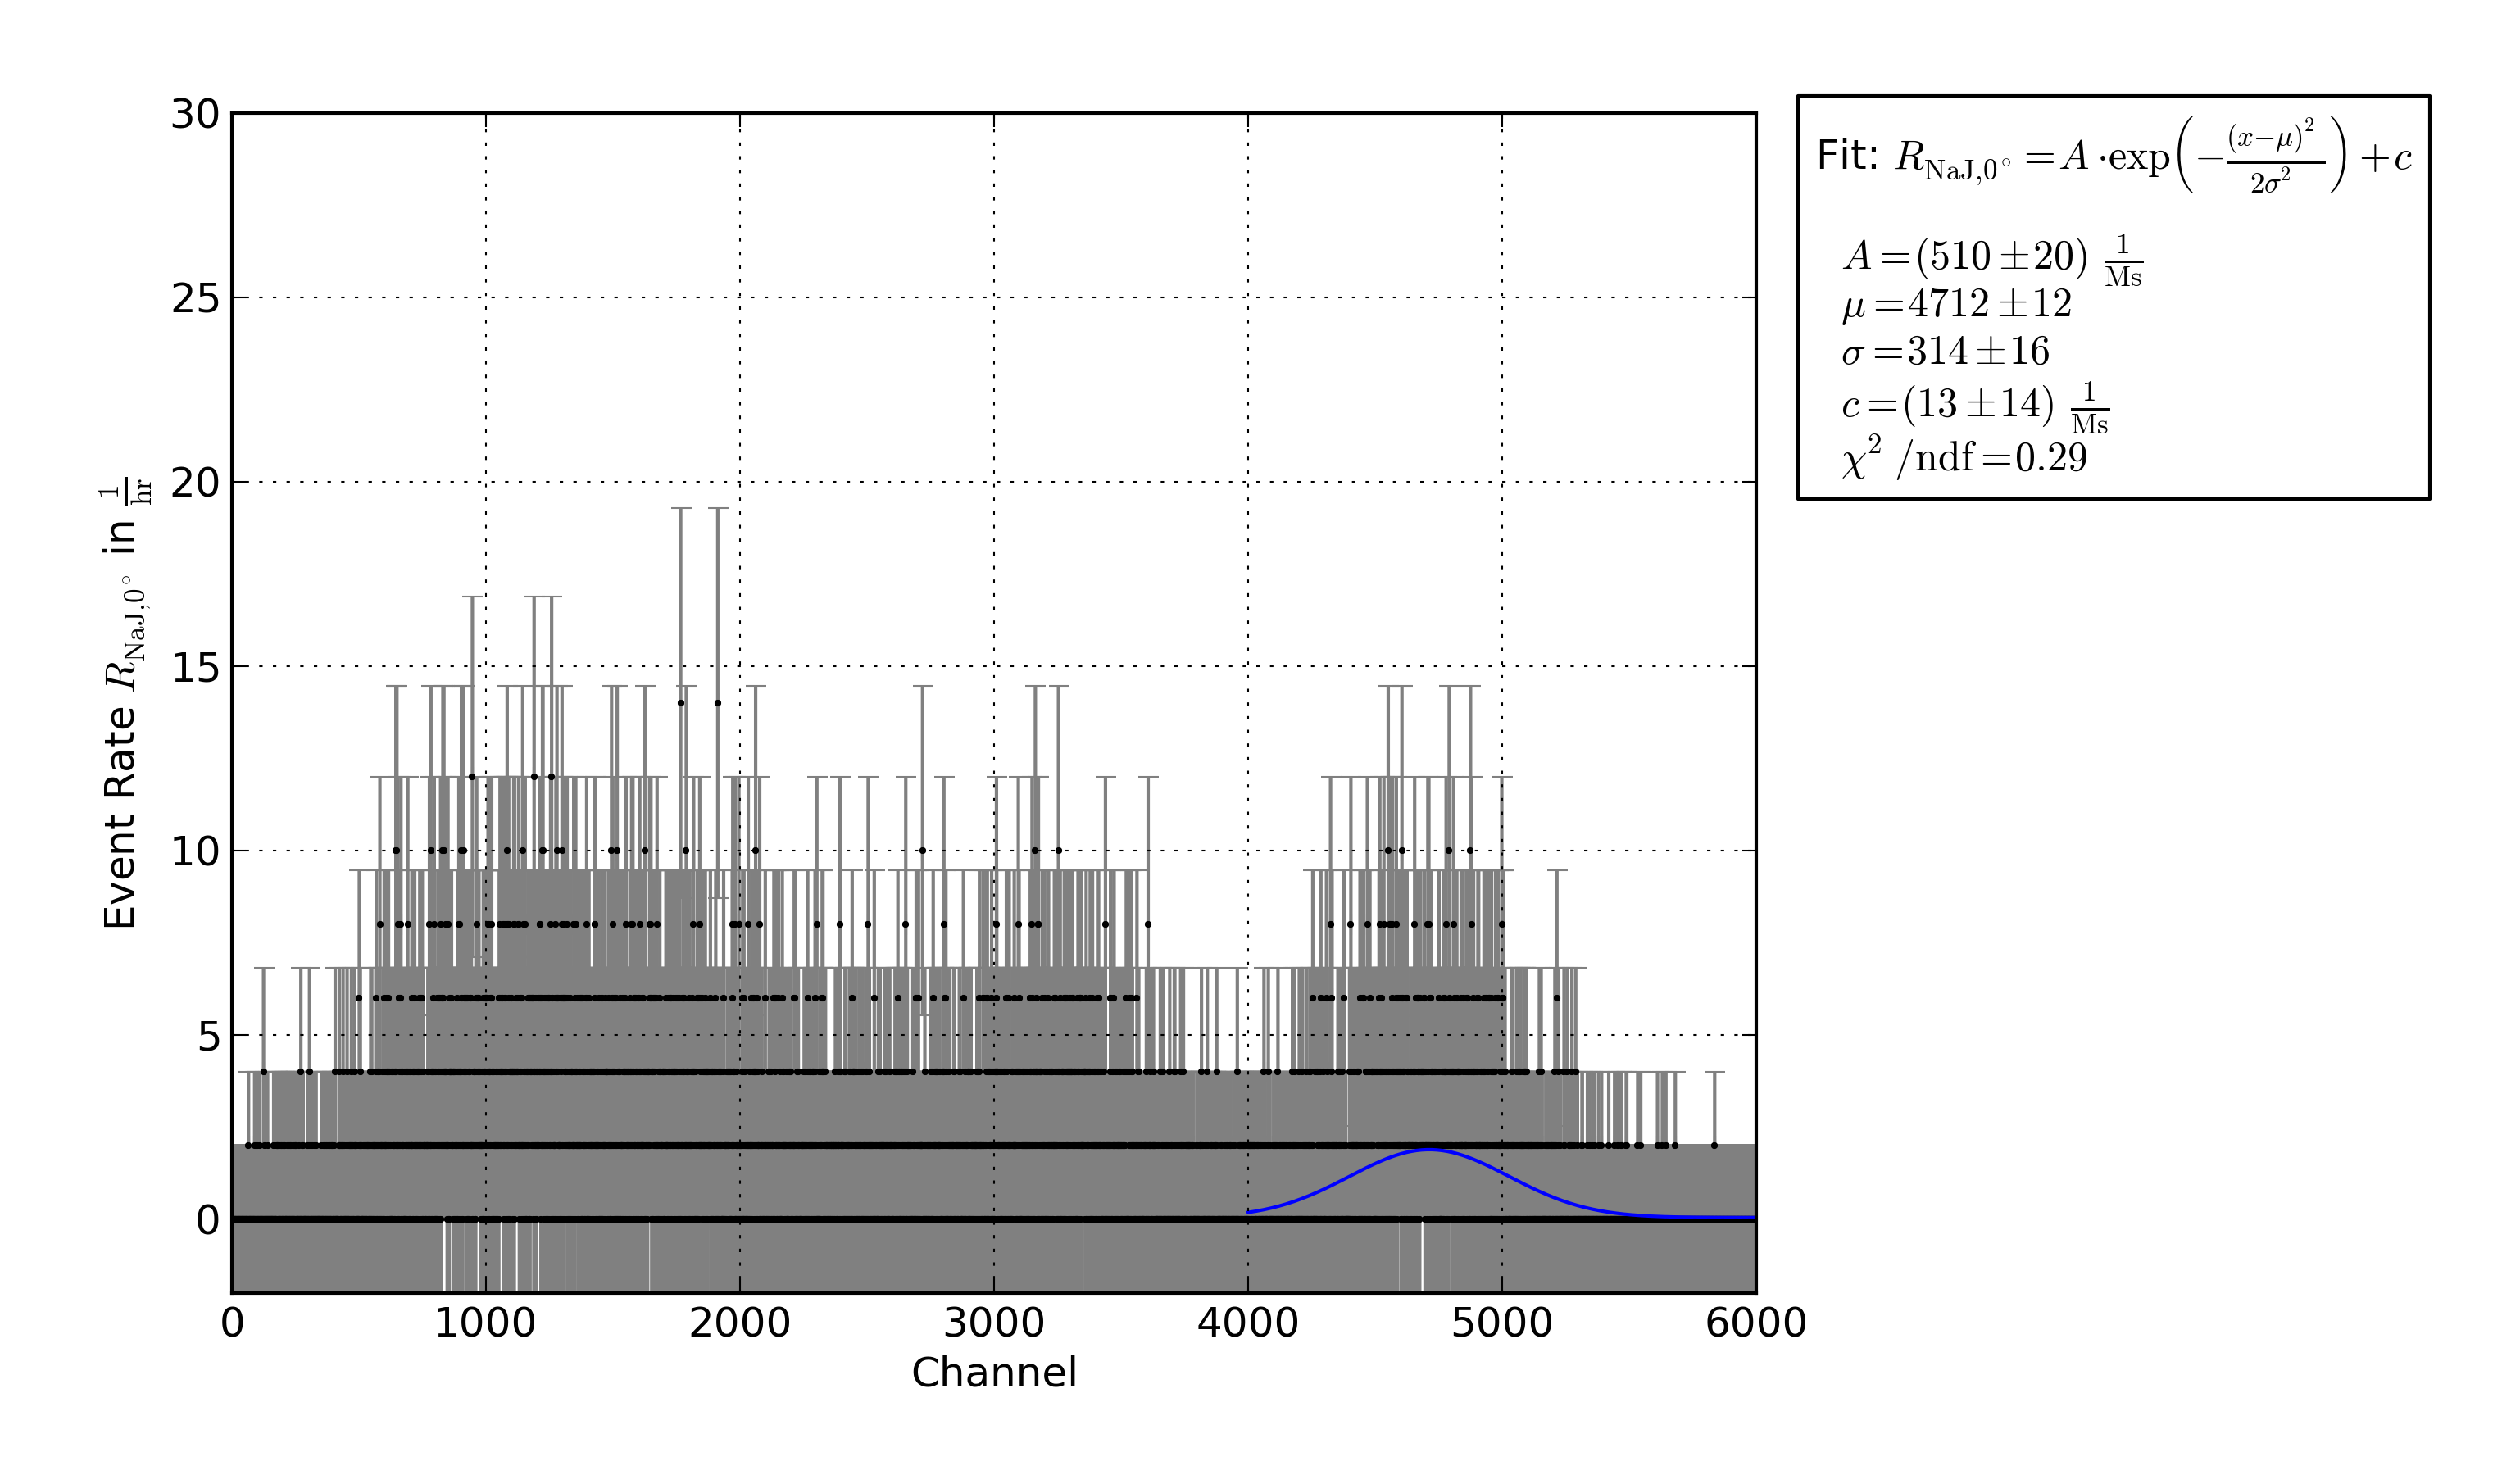
\includegraphics[width=0.6\textwidth]{plots/naj_0.png}
  \caption{Photon energy spectrum (NaI scintillator) of coincident signals
  with $\theta=0\degree$. Measurement duration $t=1800\mathrm{s}$.}
  \label{fig:naj0}
\end{figure}
\begin{figure}[h!]
  \centering
  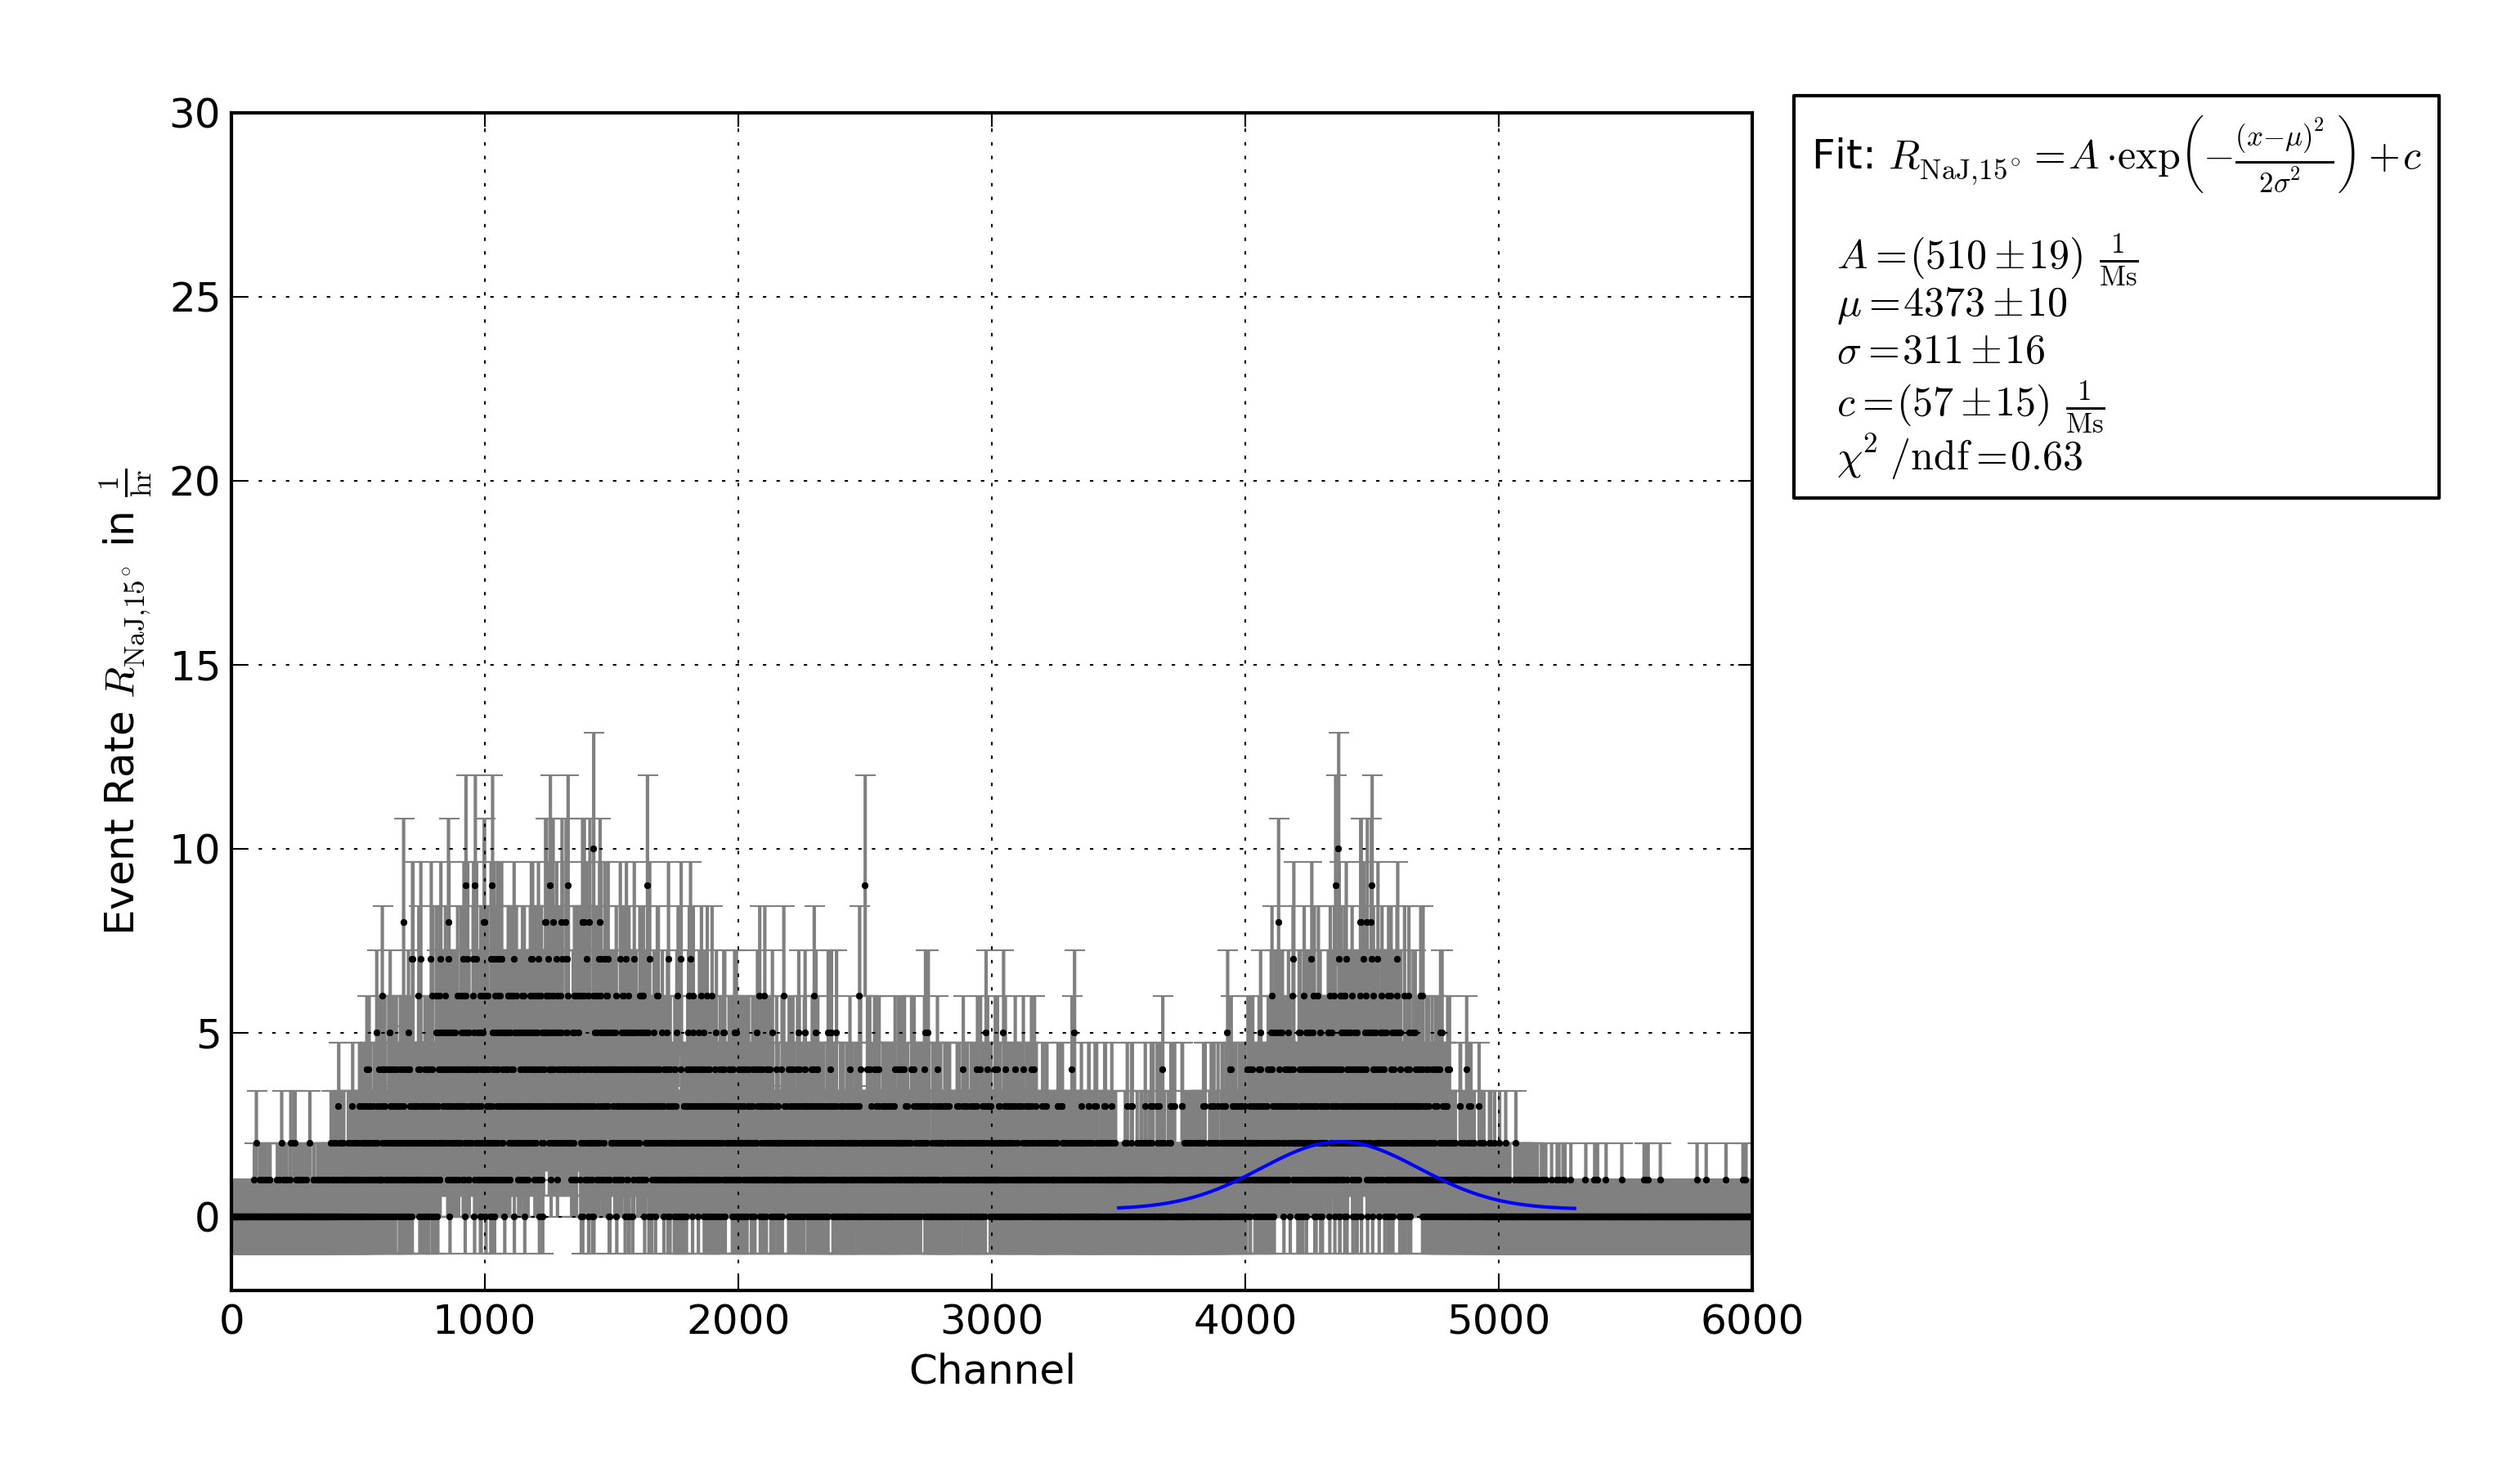
\includegraphics[width=0.6\textwidth]{plots/naj_15.png}
  \caption{Photon energy spectrum (NaI scintillator) of coincident signals
  with $\theta=15\degree$. Measurement duration $t=3600\mathrm{s}$.}
  \label{fig:naj15}
\end{figure}
\begin{figure}[h!]
  \centering
  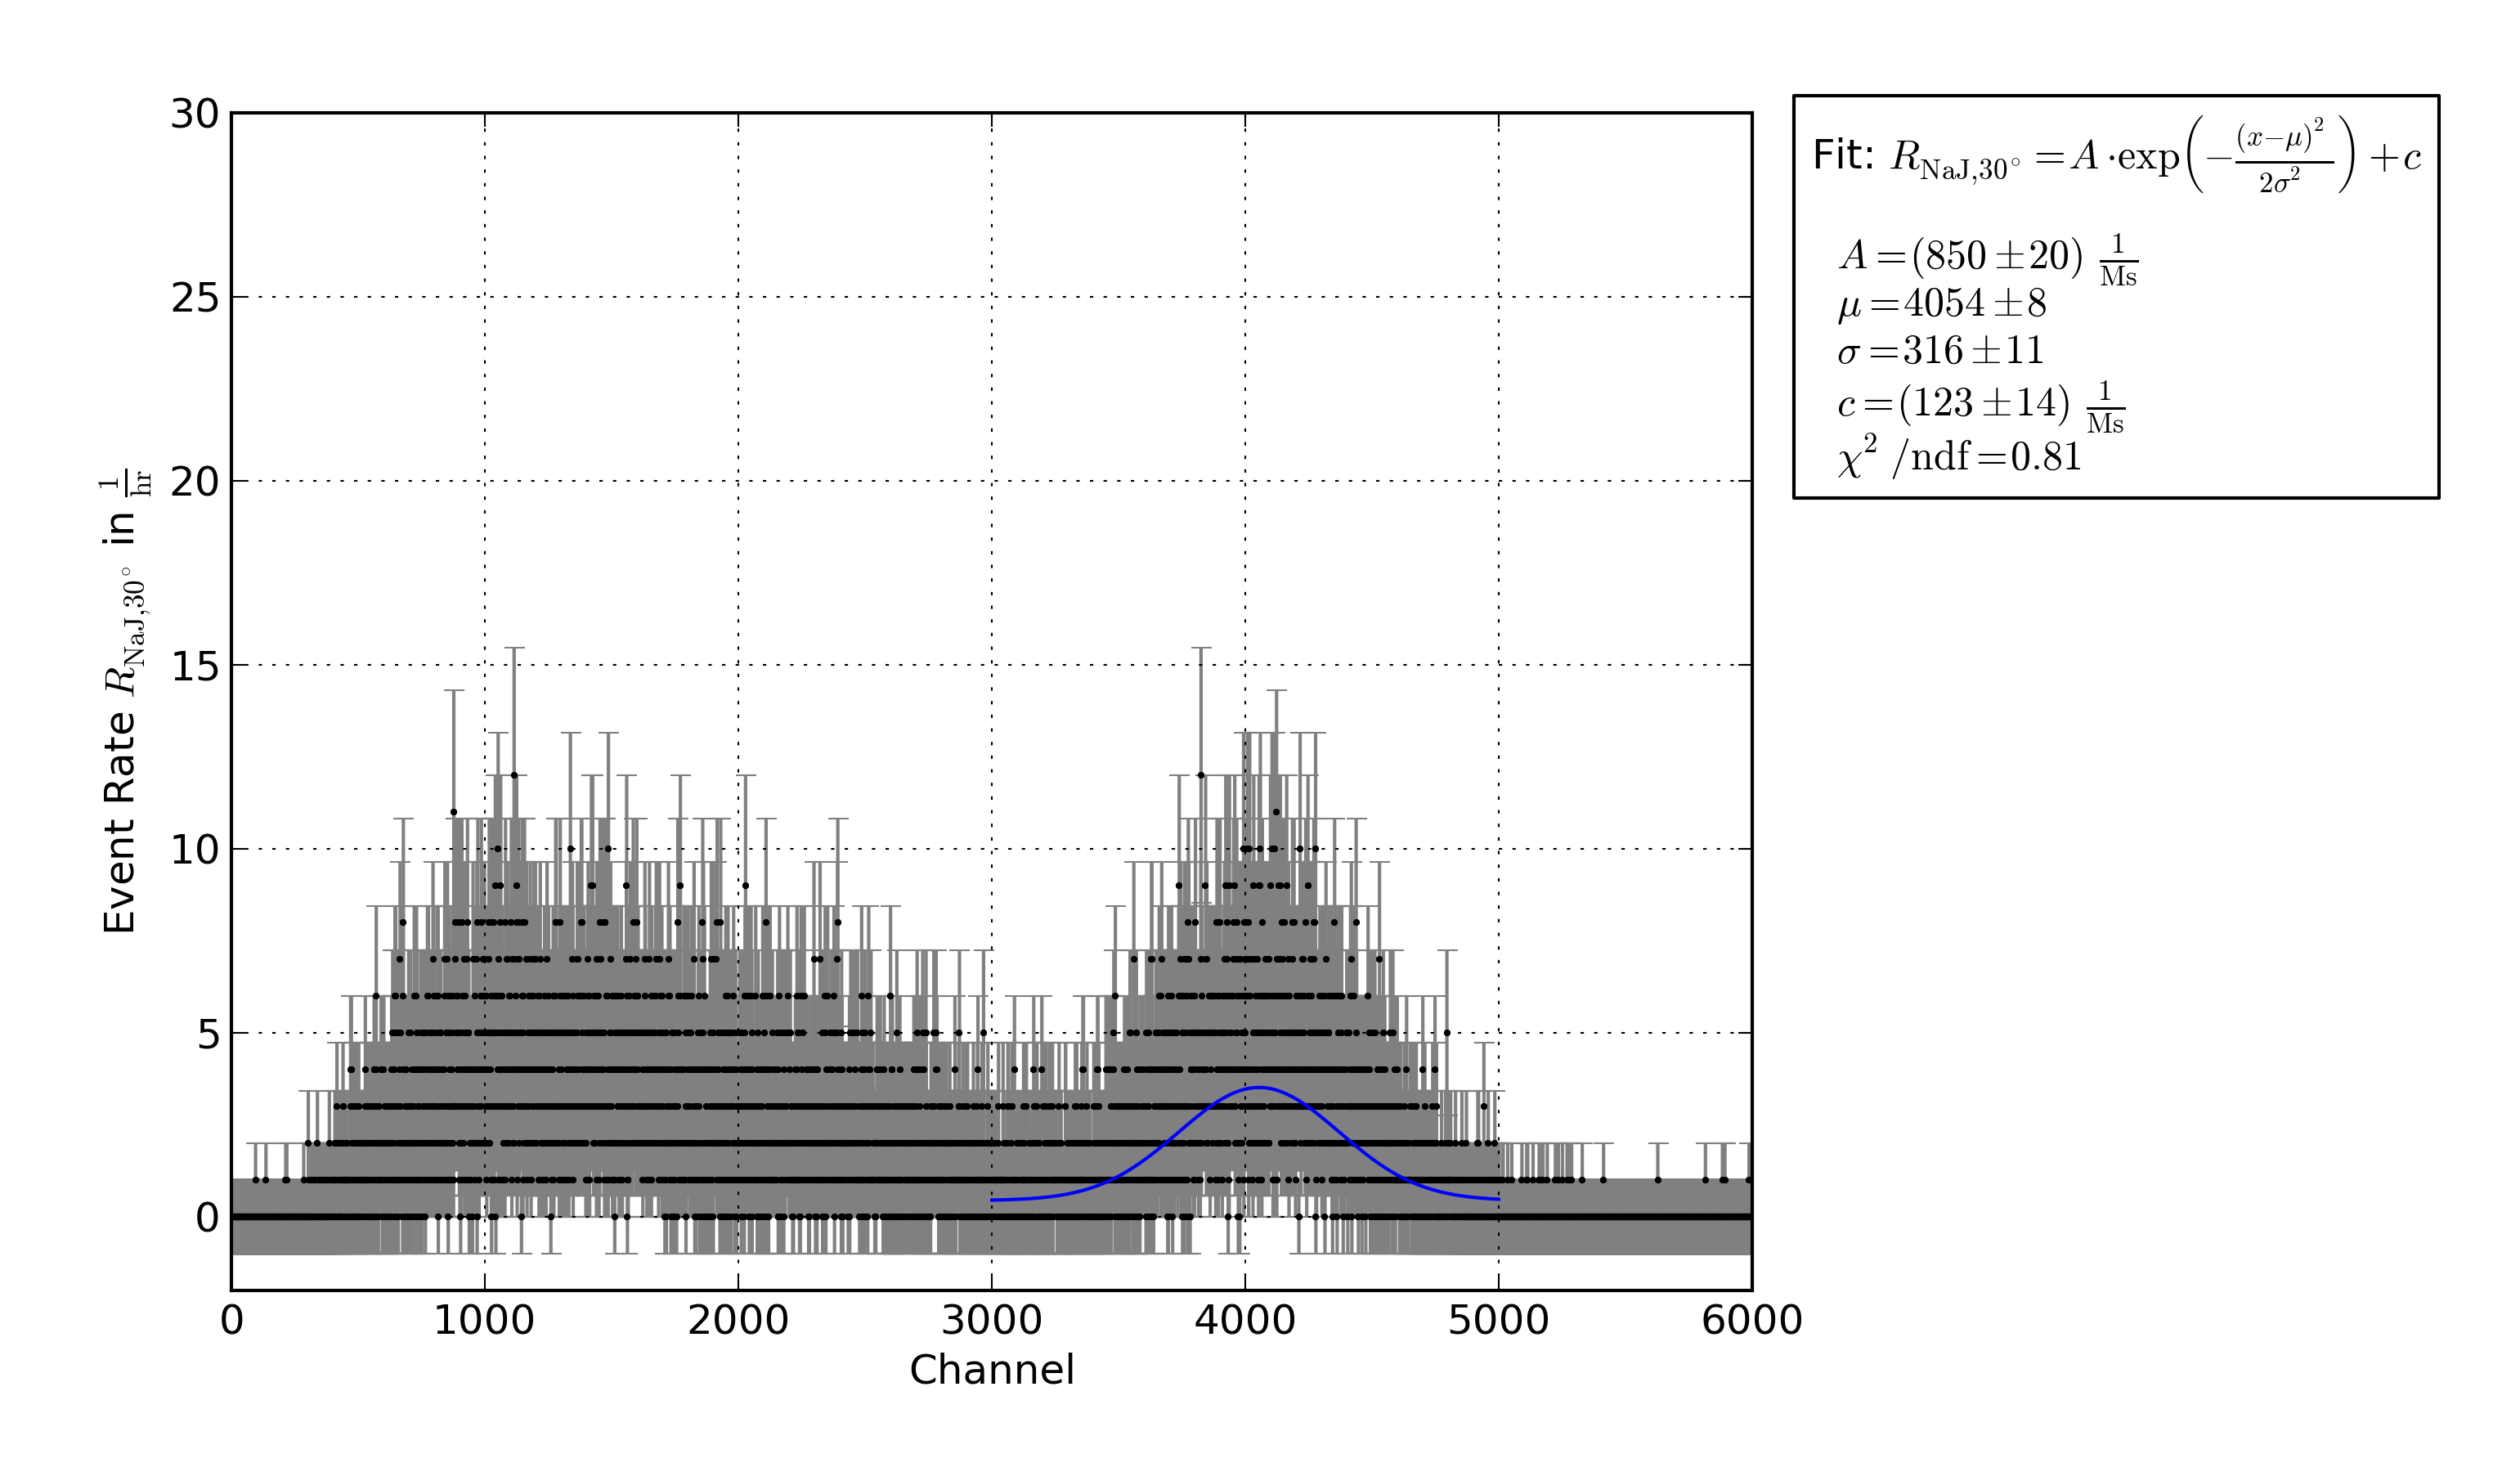
\includegraphics[width=0.6\textwidth]{plots/naj_30.png}
  \caption{Photon energy spectrum (NaI scintillator) of coincident signals
  with $\theta=30\degree$. Measurement duration $t=3600\mathrm{s}$.}
  \label{fig:naj30}
\end{figure}
\begin{figure}[h!]
  \centering
  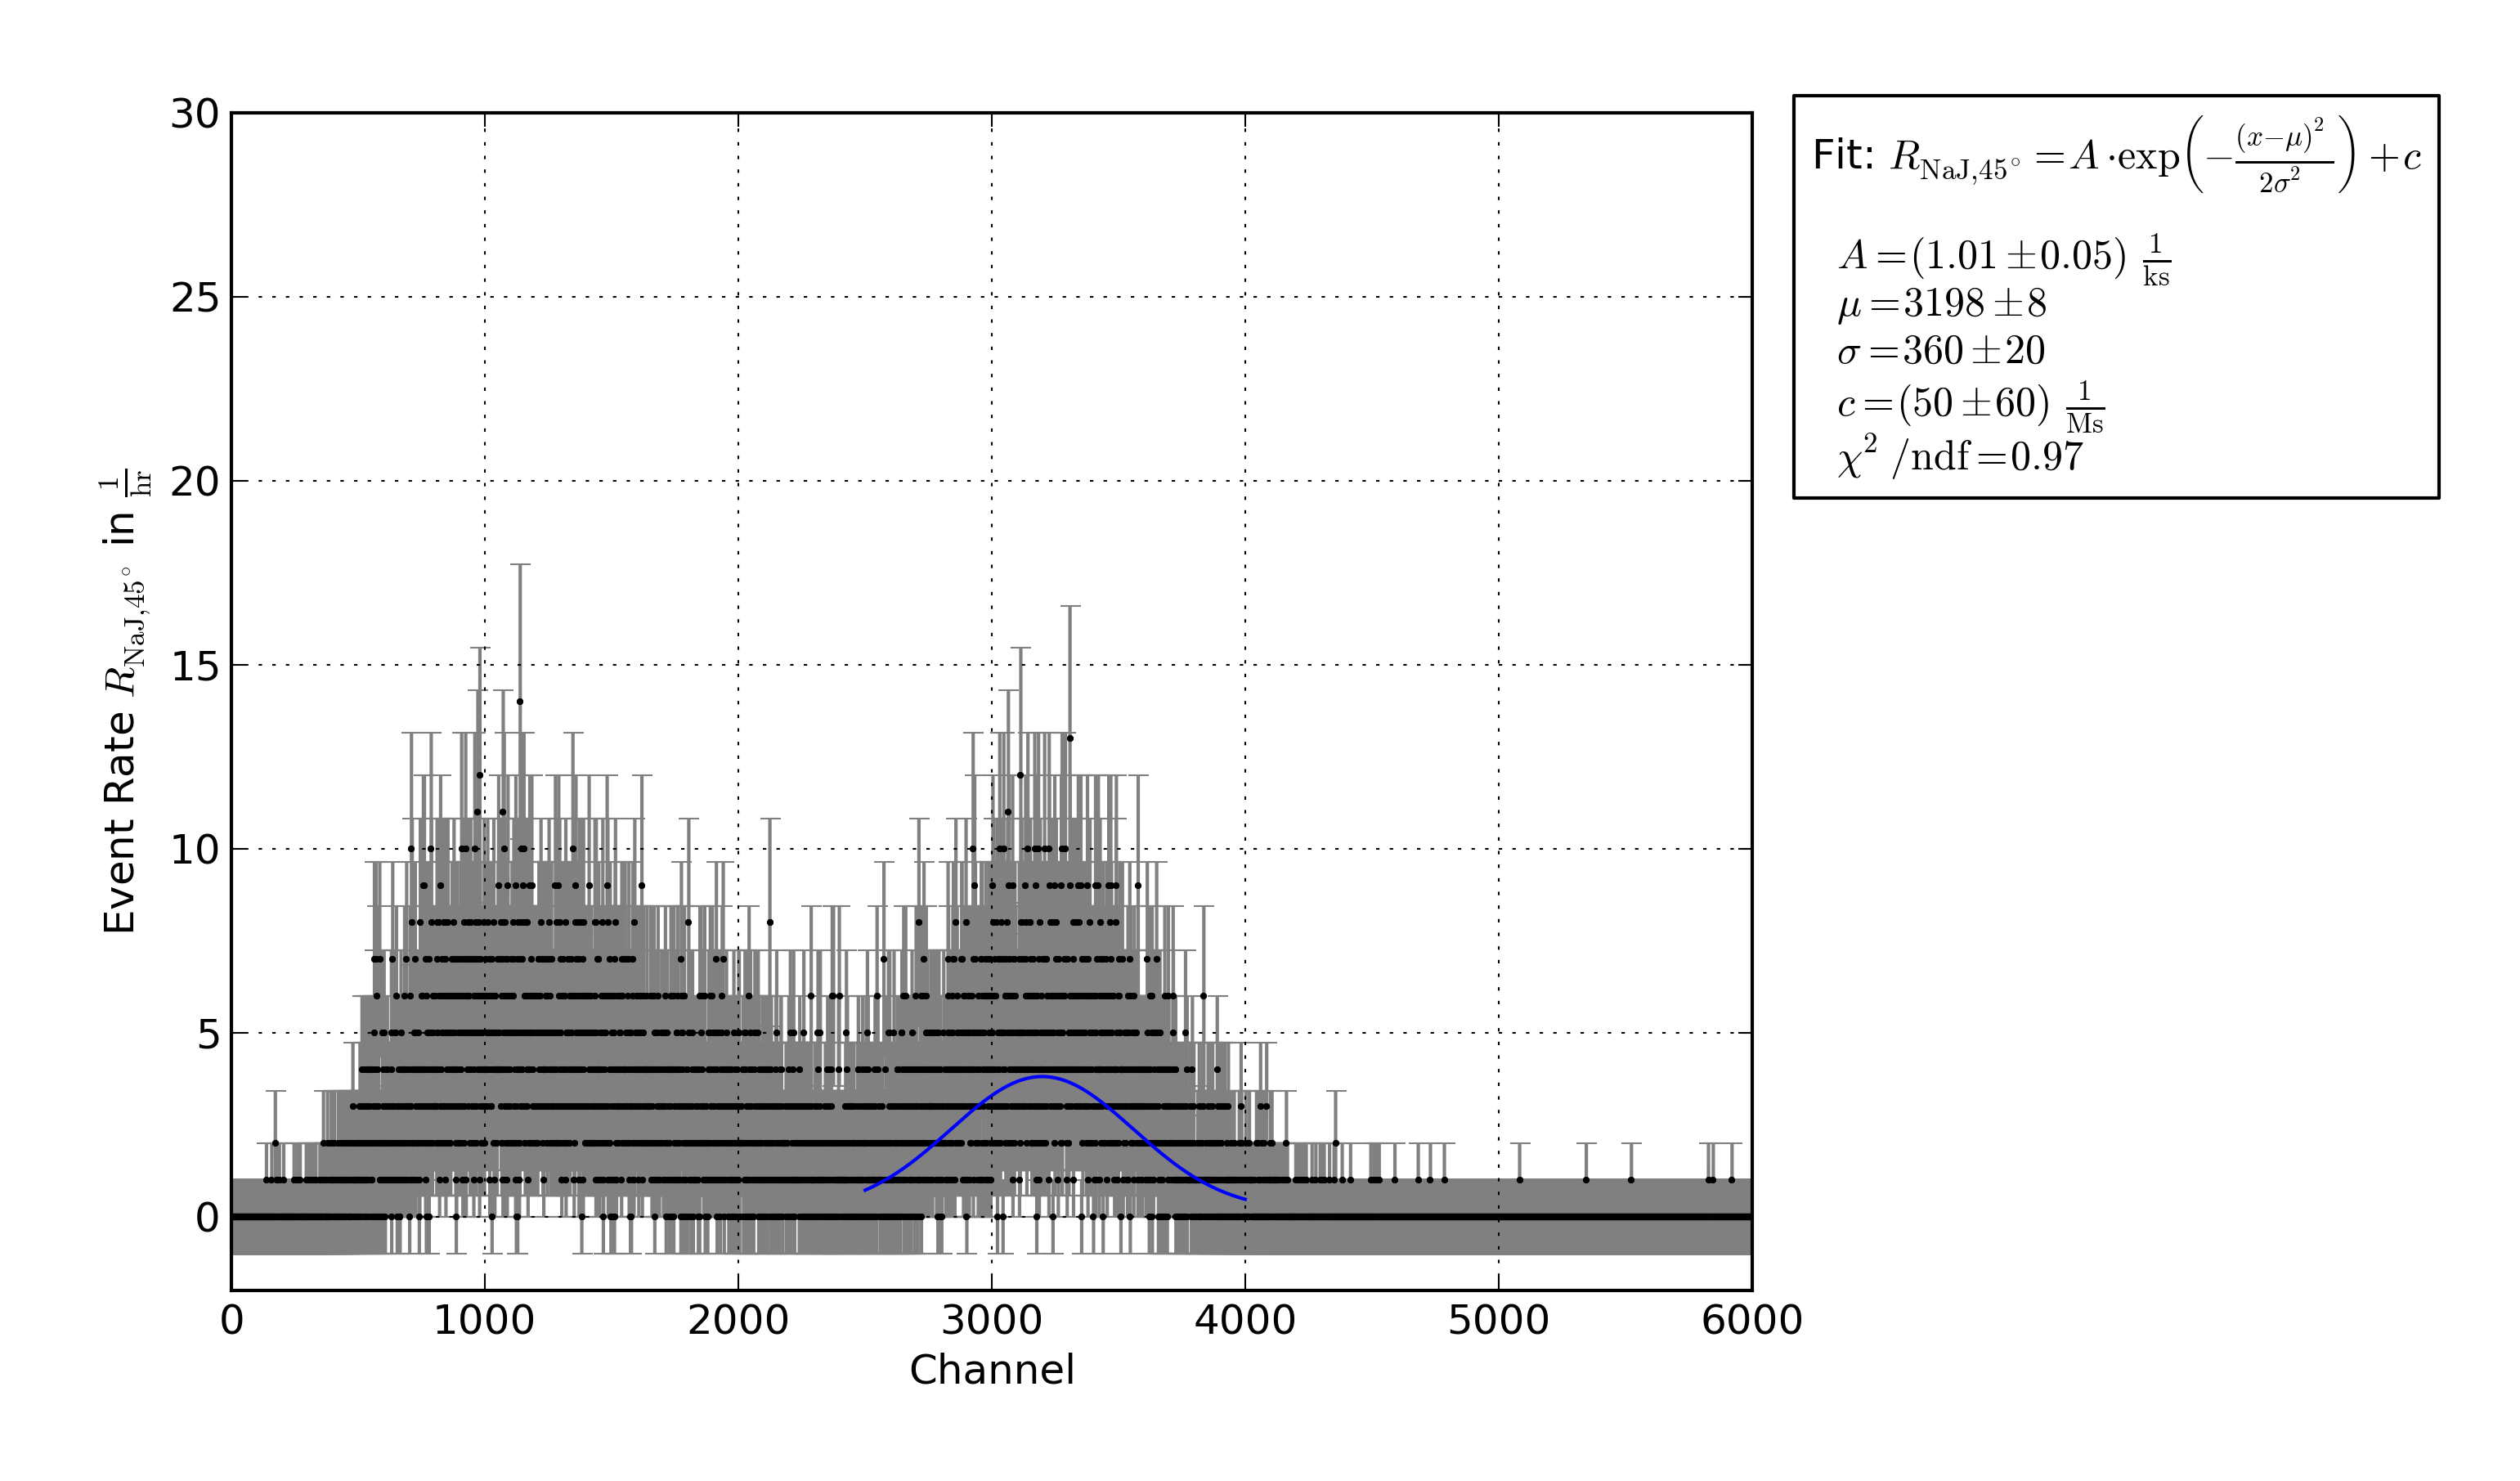
\includegraphics[width=0.6\textwidth]{plots/naj_45.png}
  \caption{Photon energy spectrum (NaI scintillator) of coincident signals
  with $\theta=45\degree$. Measurement duration $t=3600\mathrm{s}$.}
  \label{fig:naj45}
\end{figure}
\begin{figure}[h!]
  \centering
  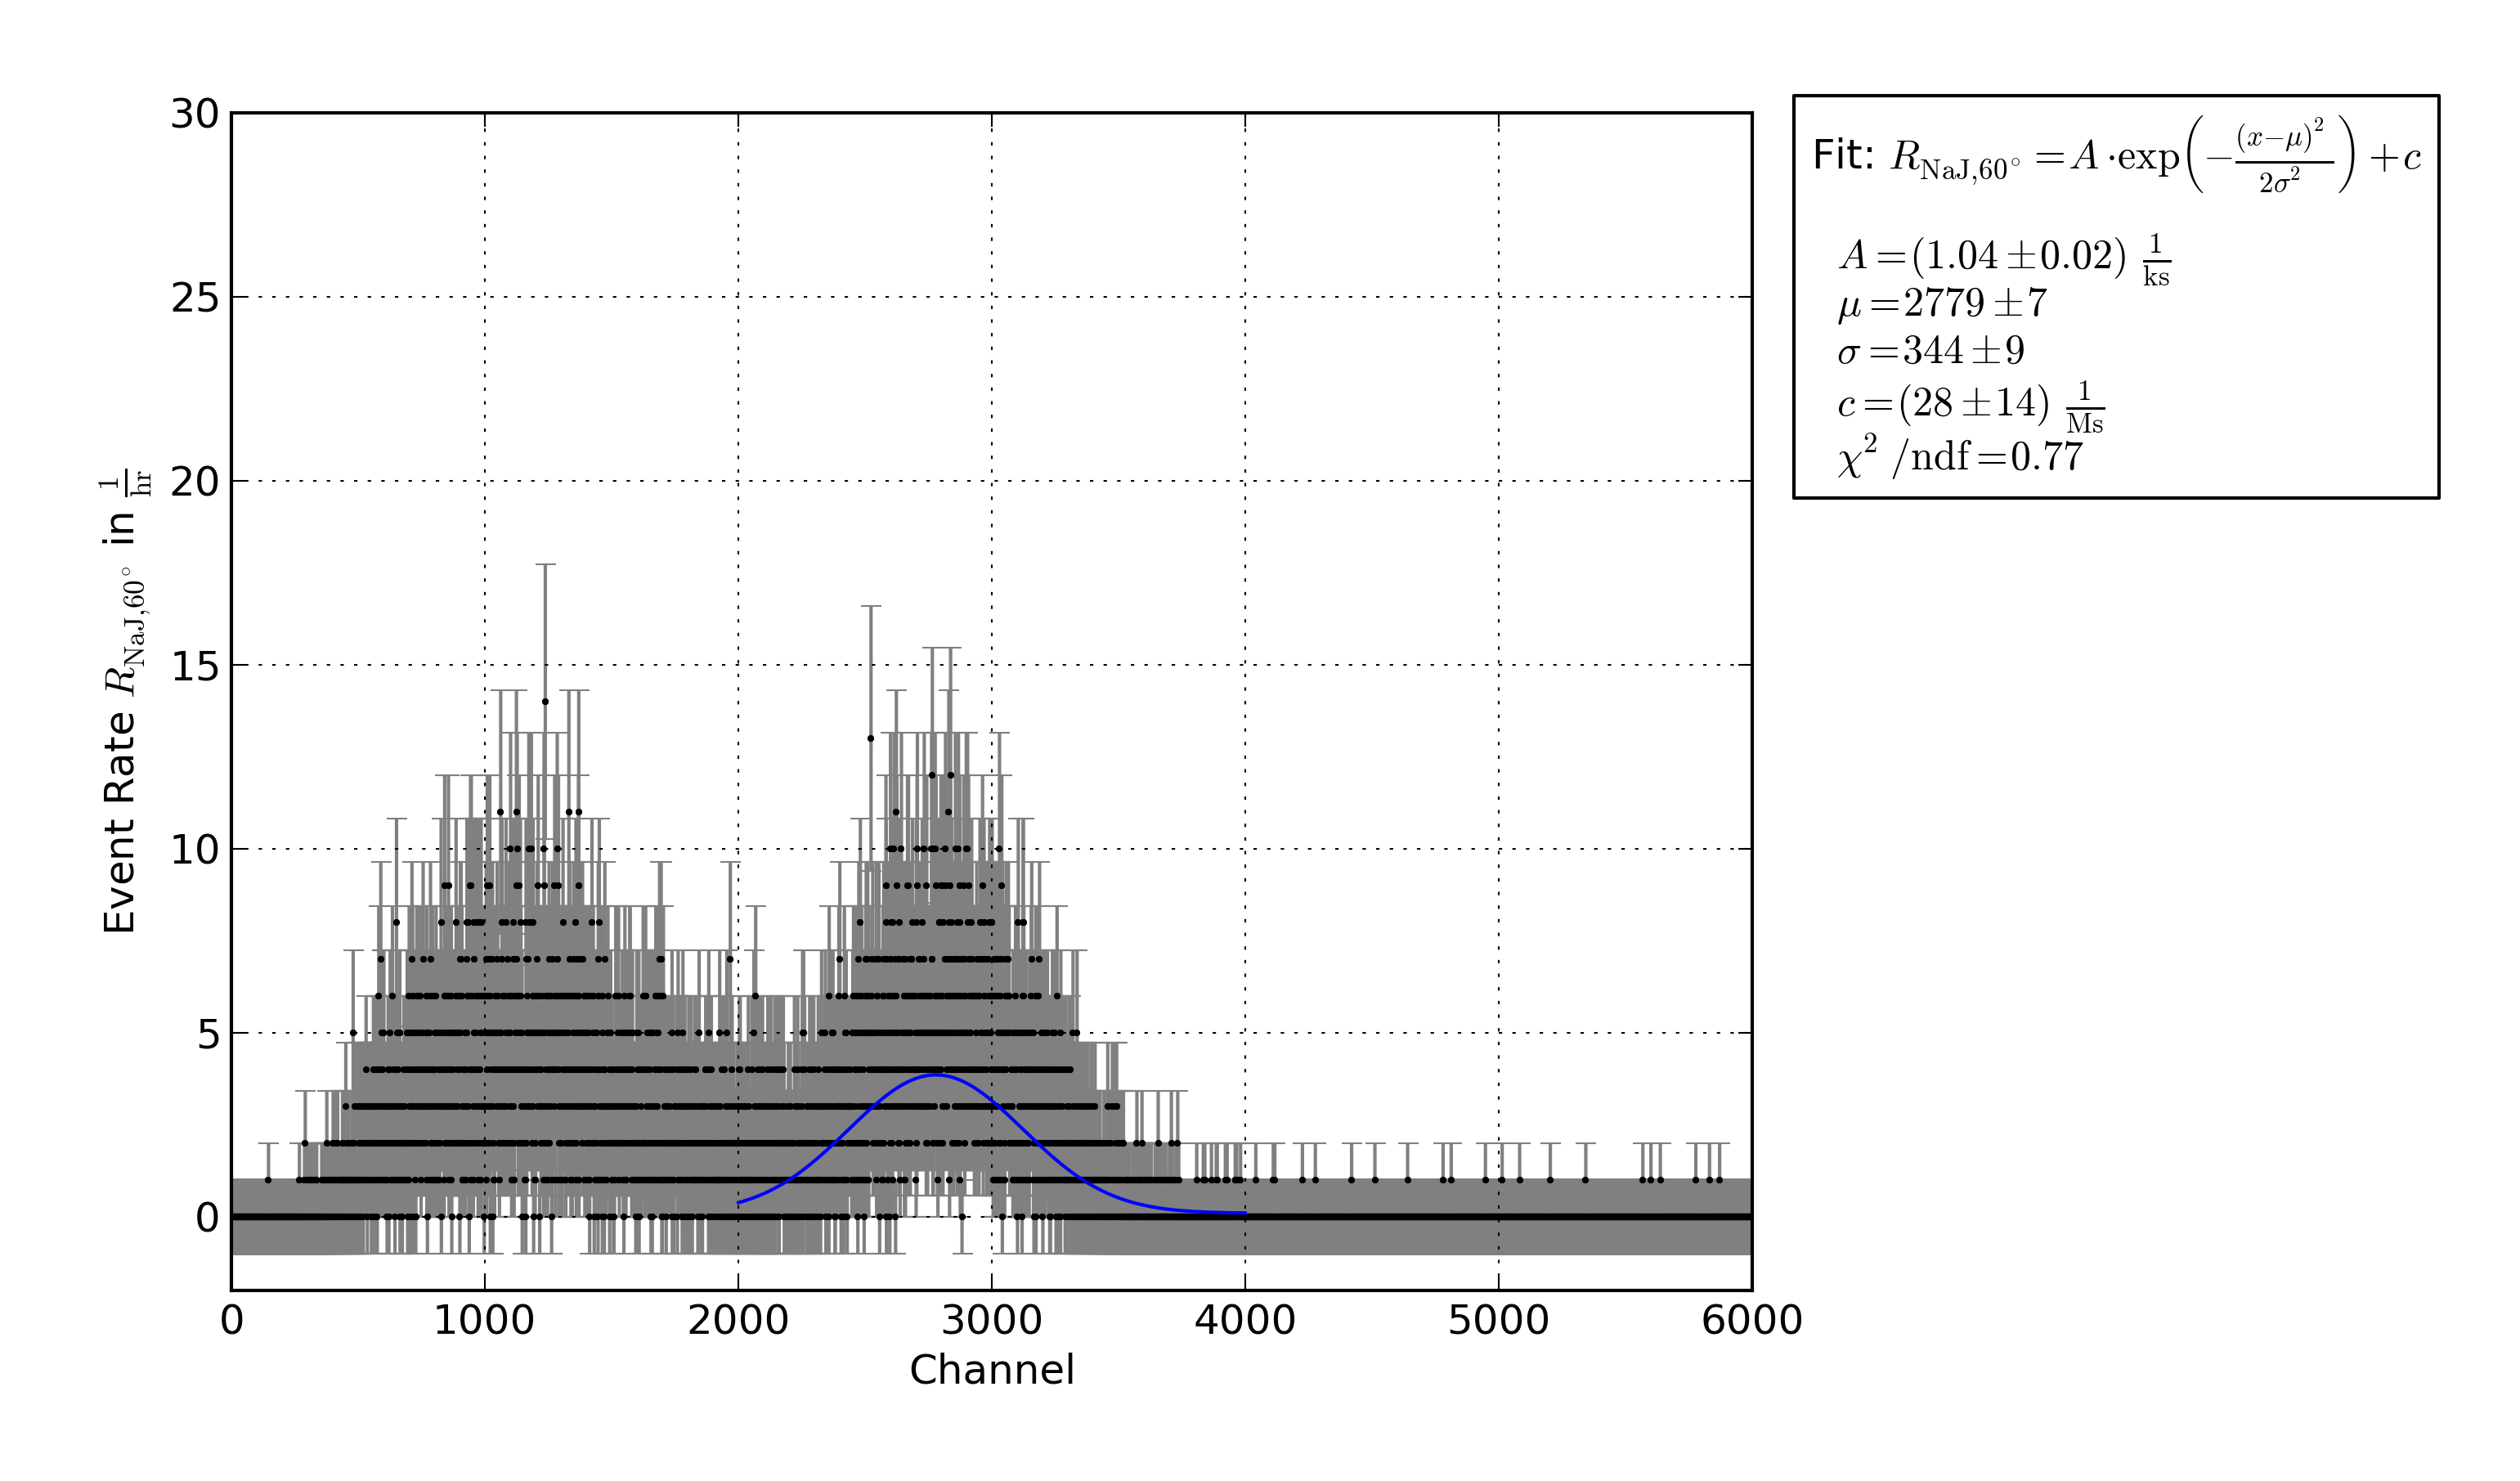
\includegraphics[width=0.6\textwidth]{plots/naj_60.png}
  \caption{Photon energy spectrum (NaI scintillator) of coincident signals
  with $\theta=60\degree$. Measurement duration $t=3600\mathrm{s}$.}
  \label{fig:naj60}
\end{figure}
\begin{figure}[h!]
  \centering
  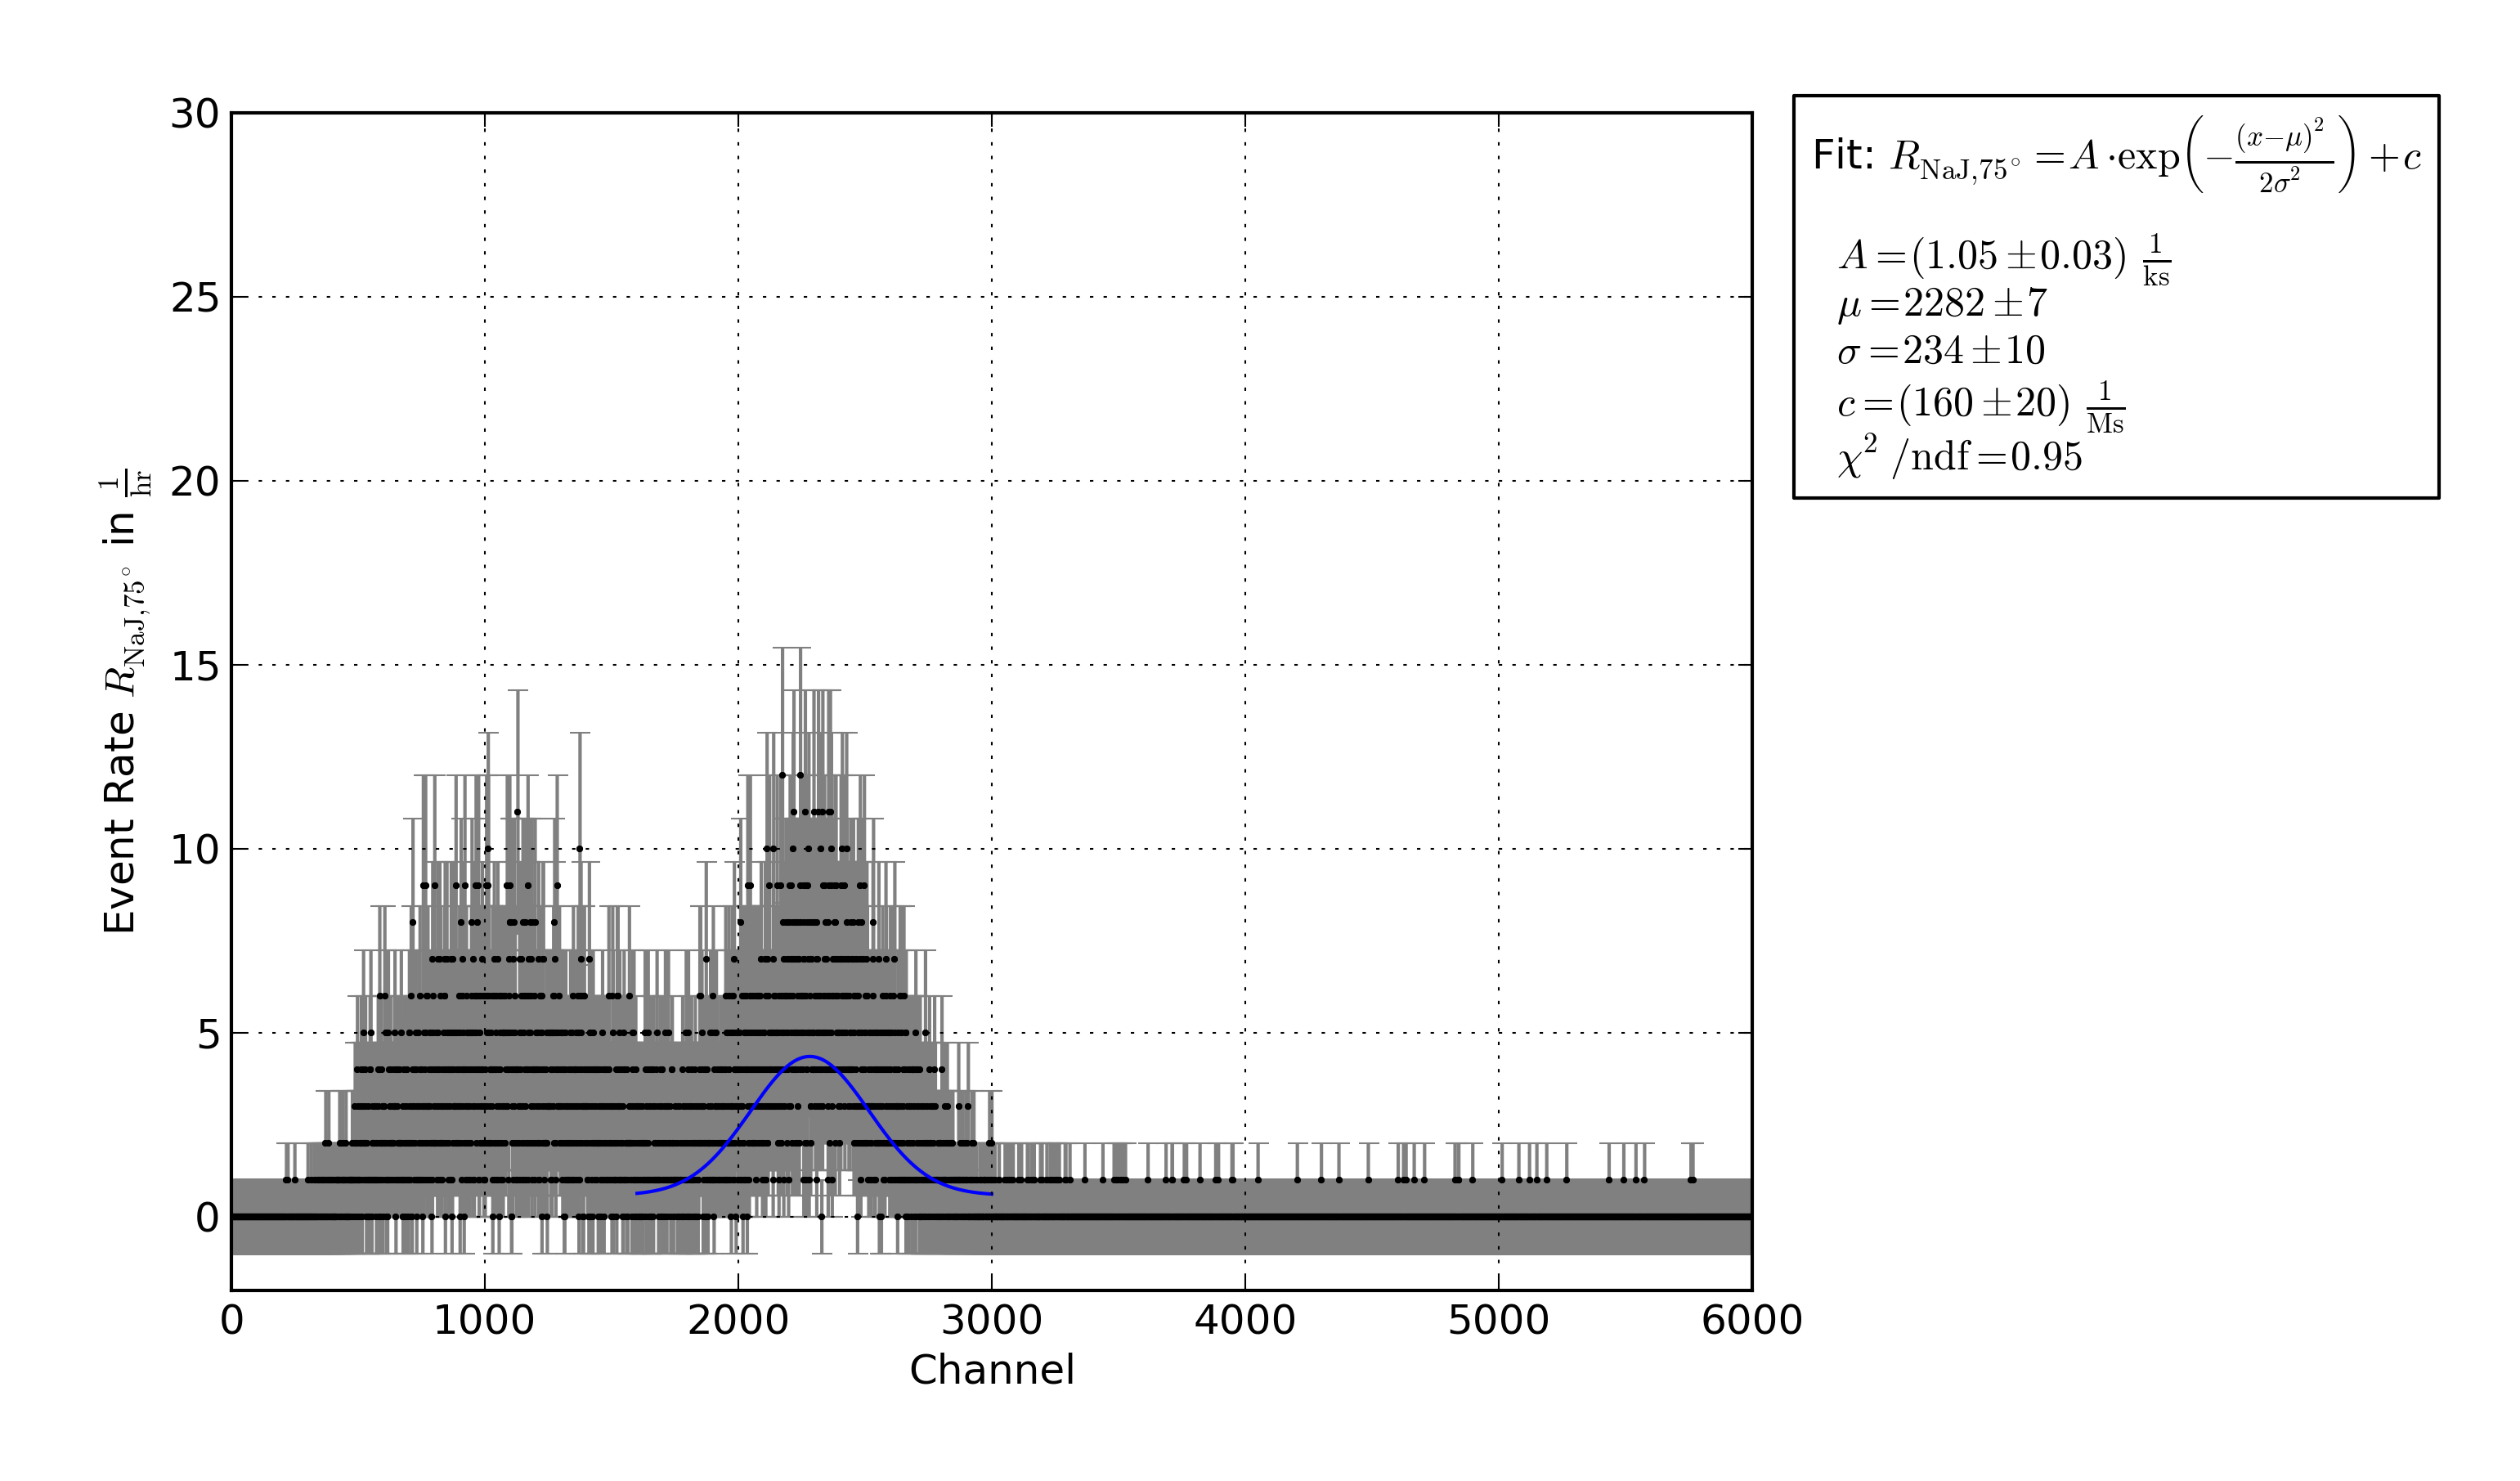
\includegraphics[width=0.6\textwidth]{plots/naj_75.png}
  \caption{Photon energy spectrum (NaI scintillator) of coincident signals
  with $\theta=75\degree$. Measurement duration $t=3600\mathrm{s}$.}
  \label{fig:naj75}
\end{figure}
\begin{figure}[h!]
  \centering
  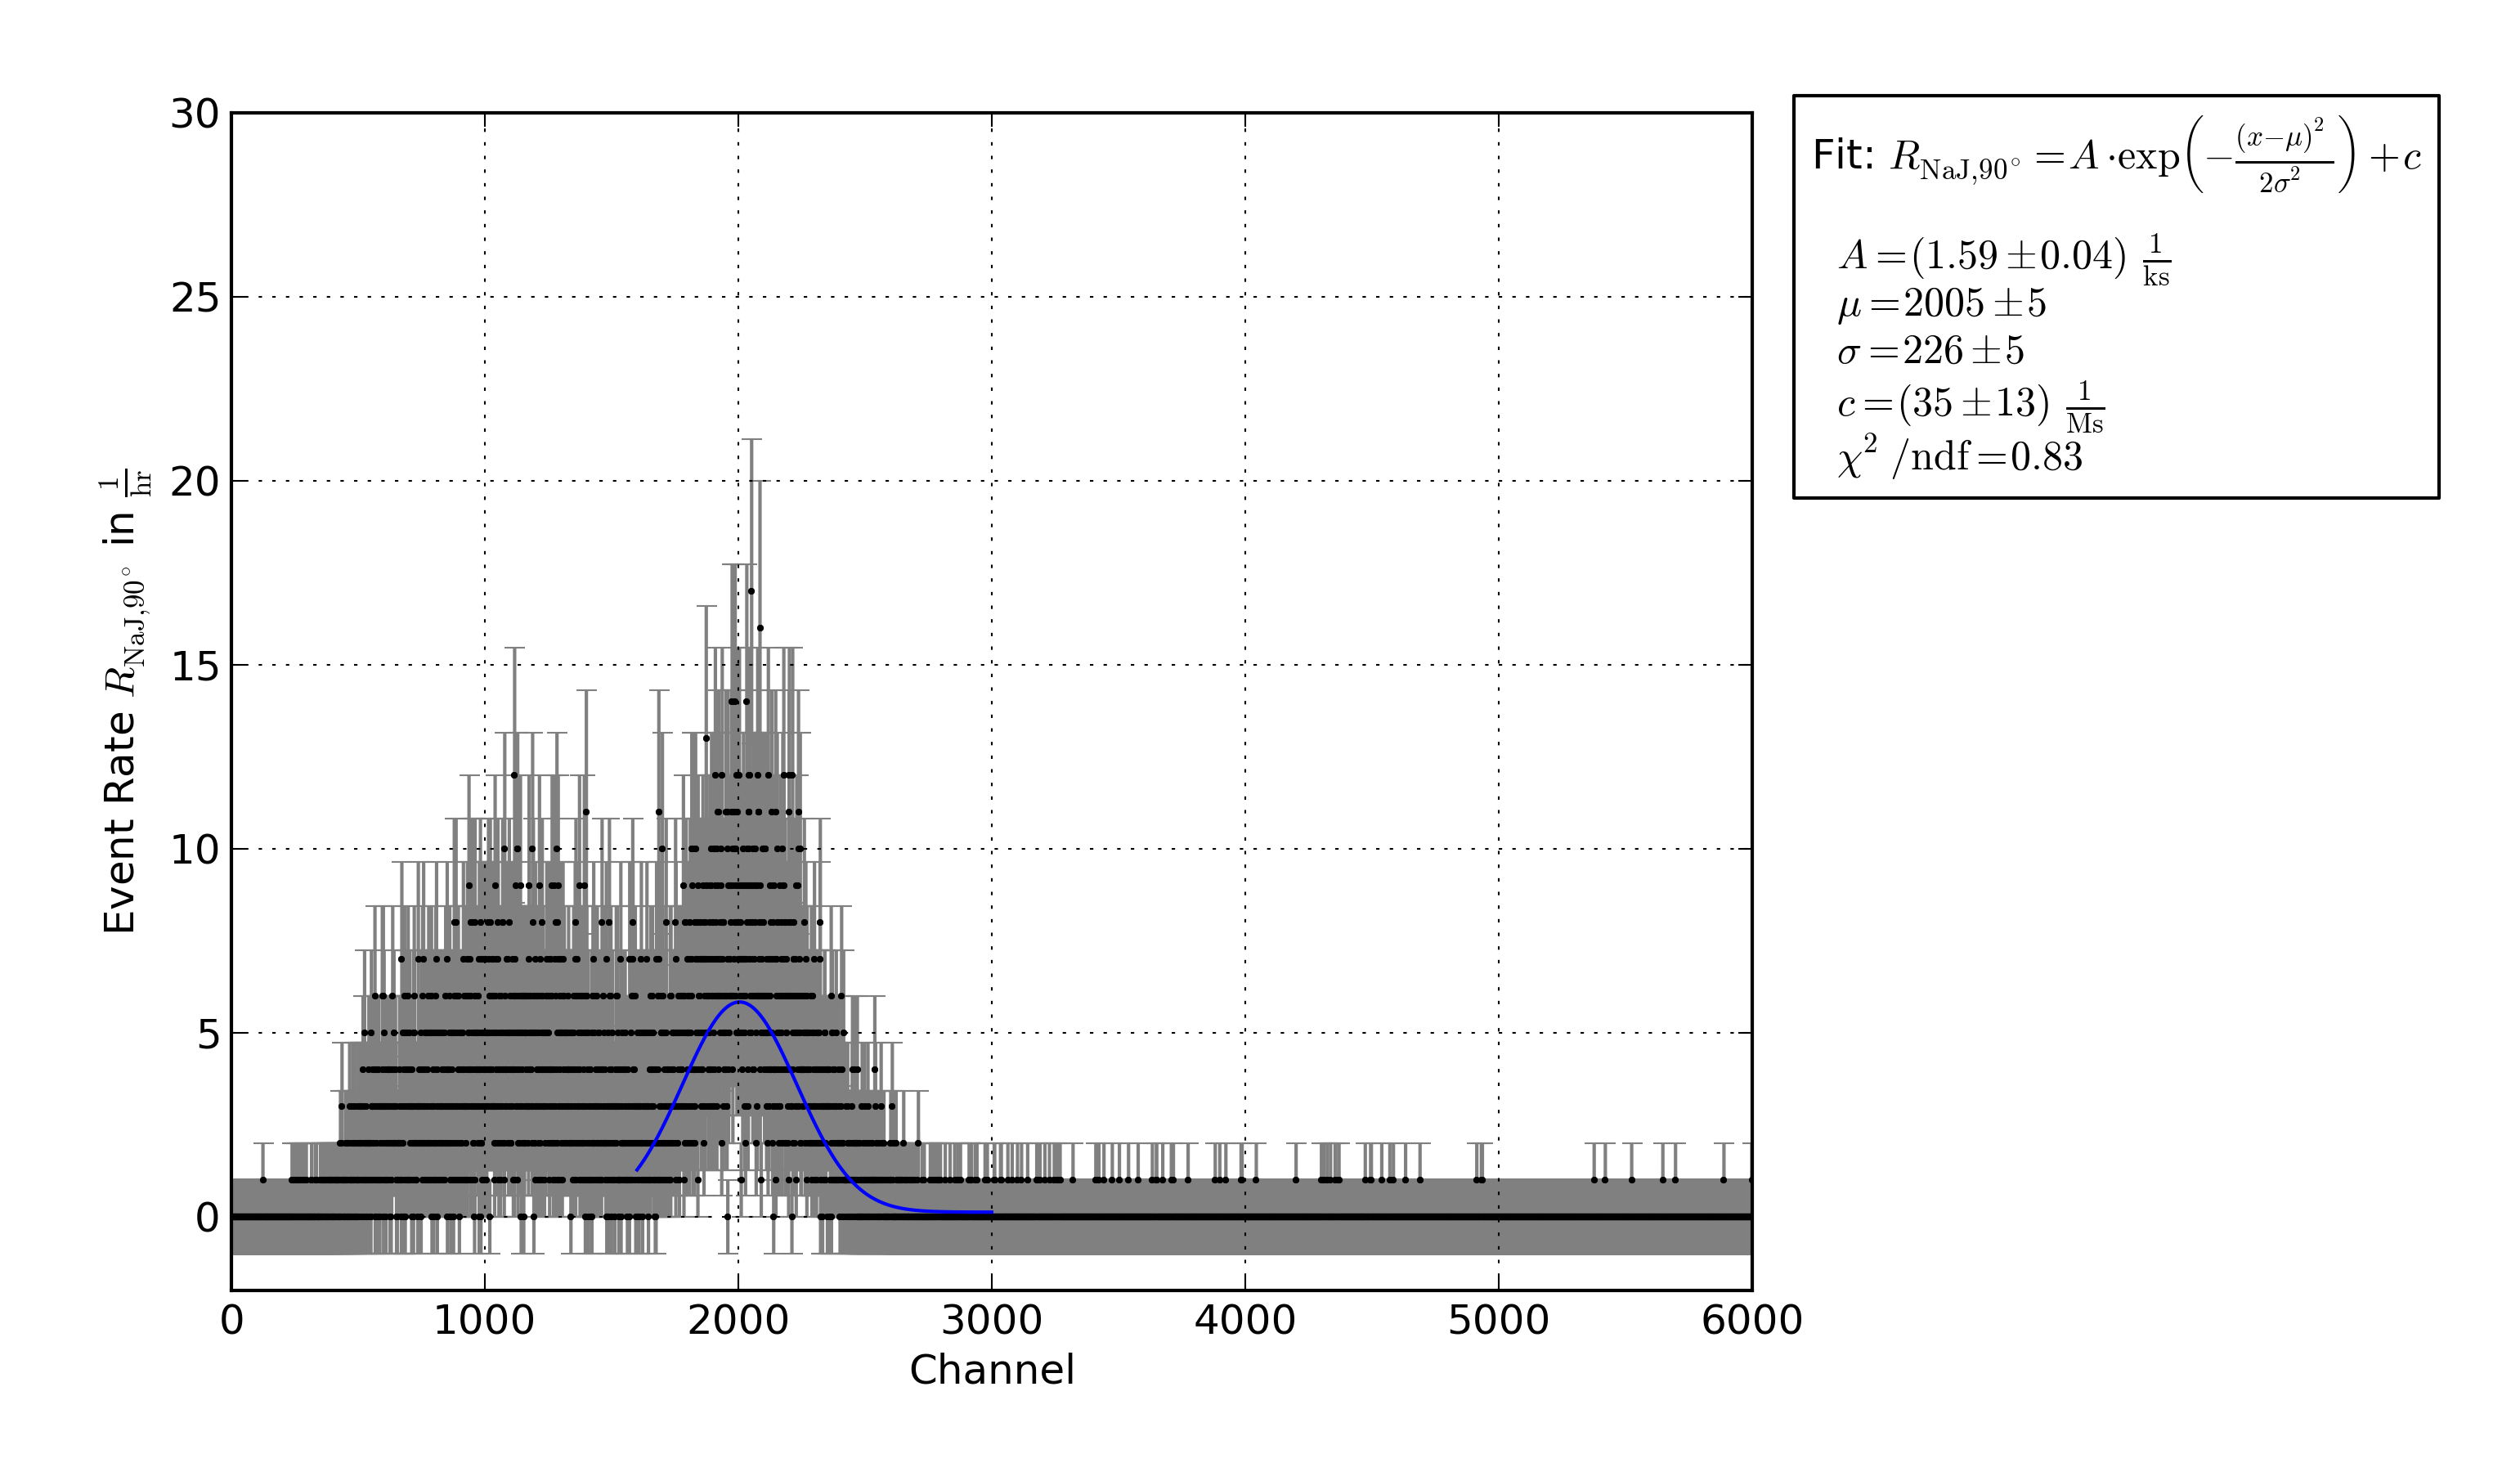
\includegraphics[width=0.6\textwidth]{plots/naj_90.png}
  \caption{Photon energy spectrum (NaI scintillator) of coincident signals
  with $\theta=90\degree$. Measurement duration $t=3600\mathrm{s}$.}
  \label{fig:naj90}
\end{figure}
\begin{figure}[h!]
  \centering
  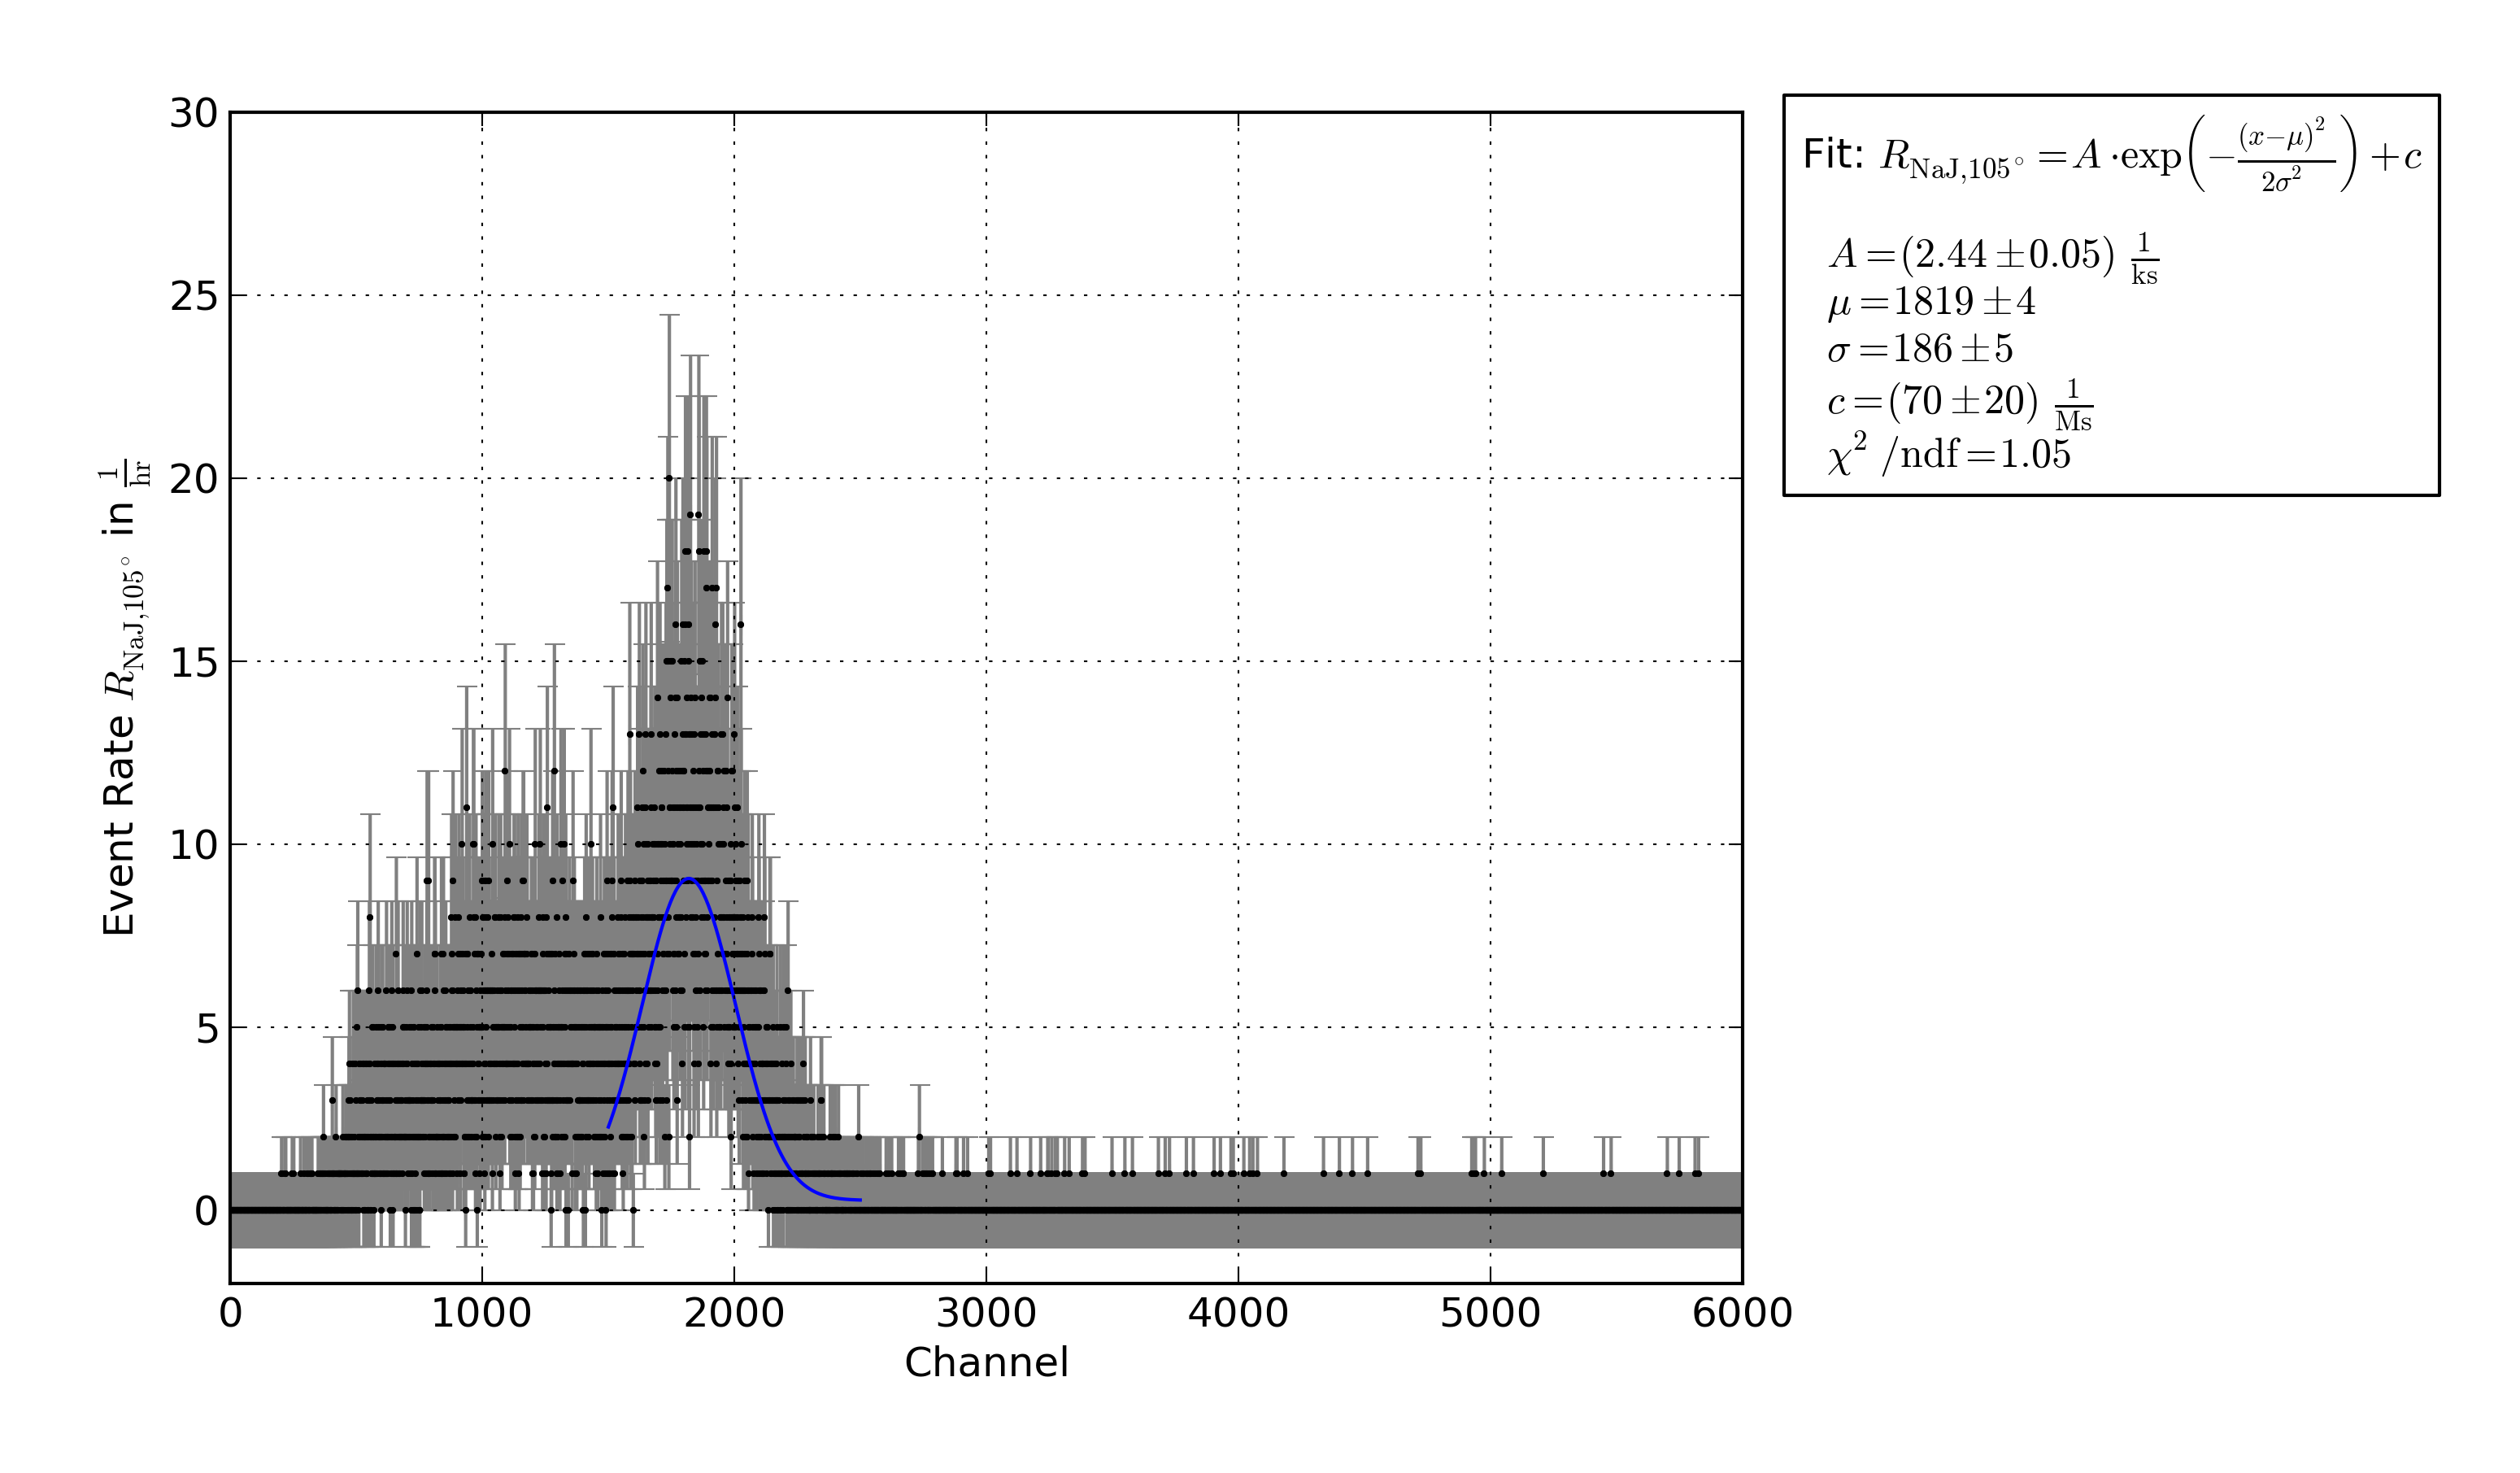
\includegraphics[width=0.6\textwidth]{plots/naj_105.png}
  \caption{Photon energy spectrum (NaI scintillator) of coincident signals
  with $\theta=105\degree$. Measurement duration $t=3600\mathrm{s}$.}
  \label{fig:naj105}
\end{figure}
\begin{figure}[h!]
  \centering
  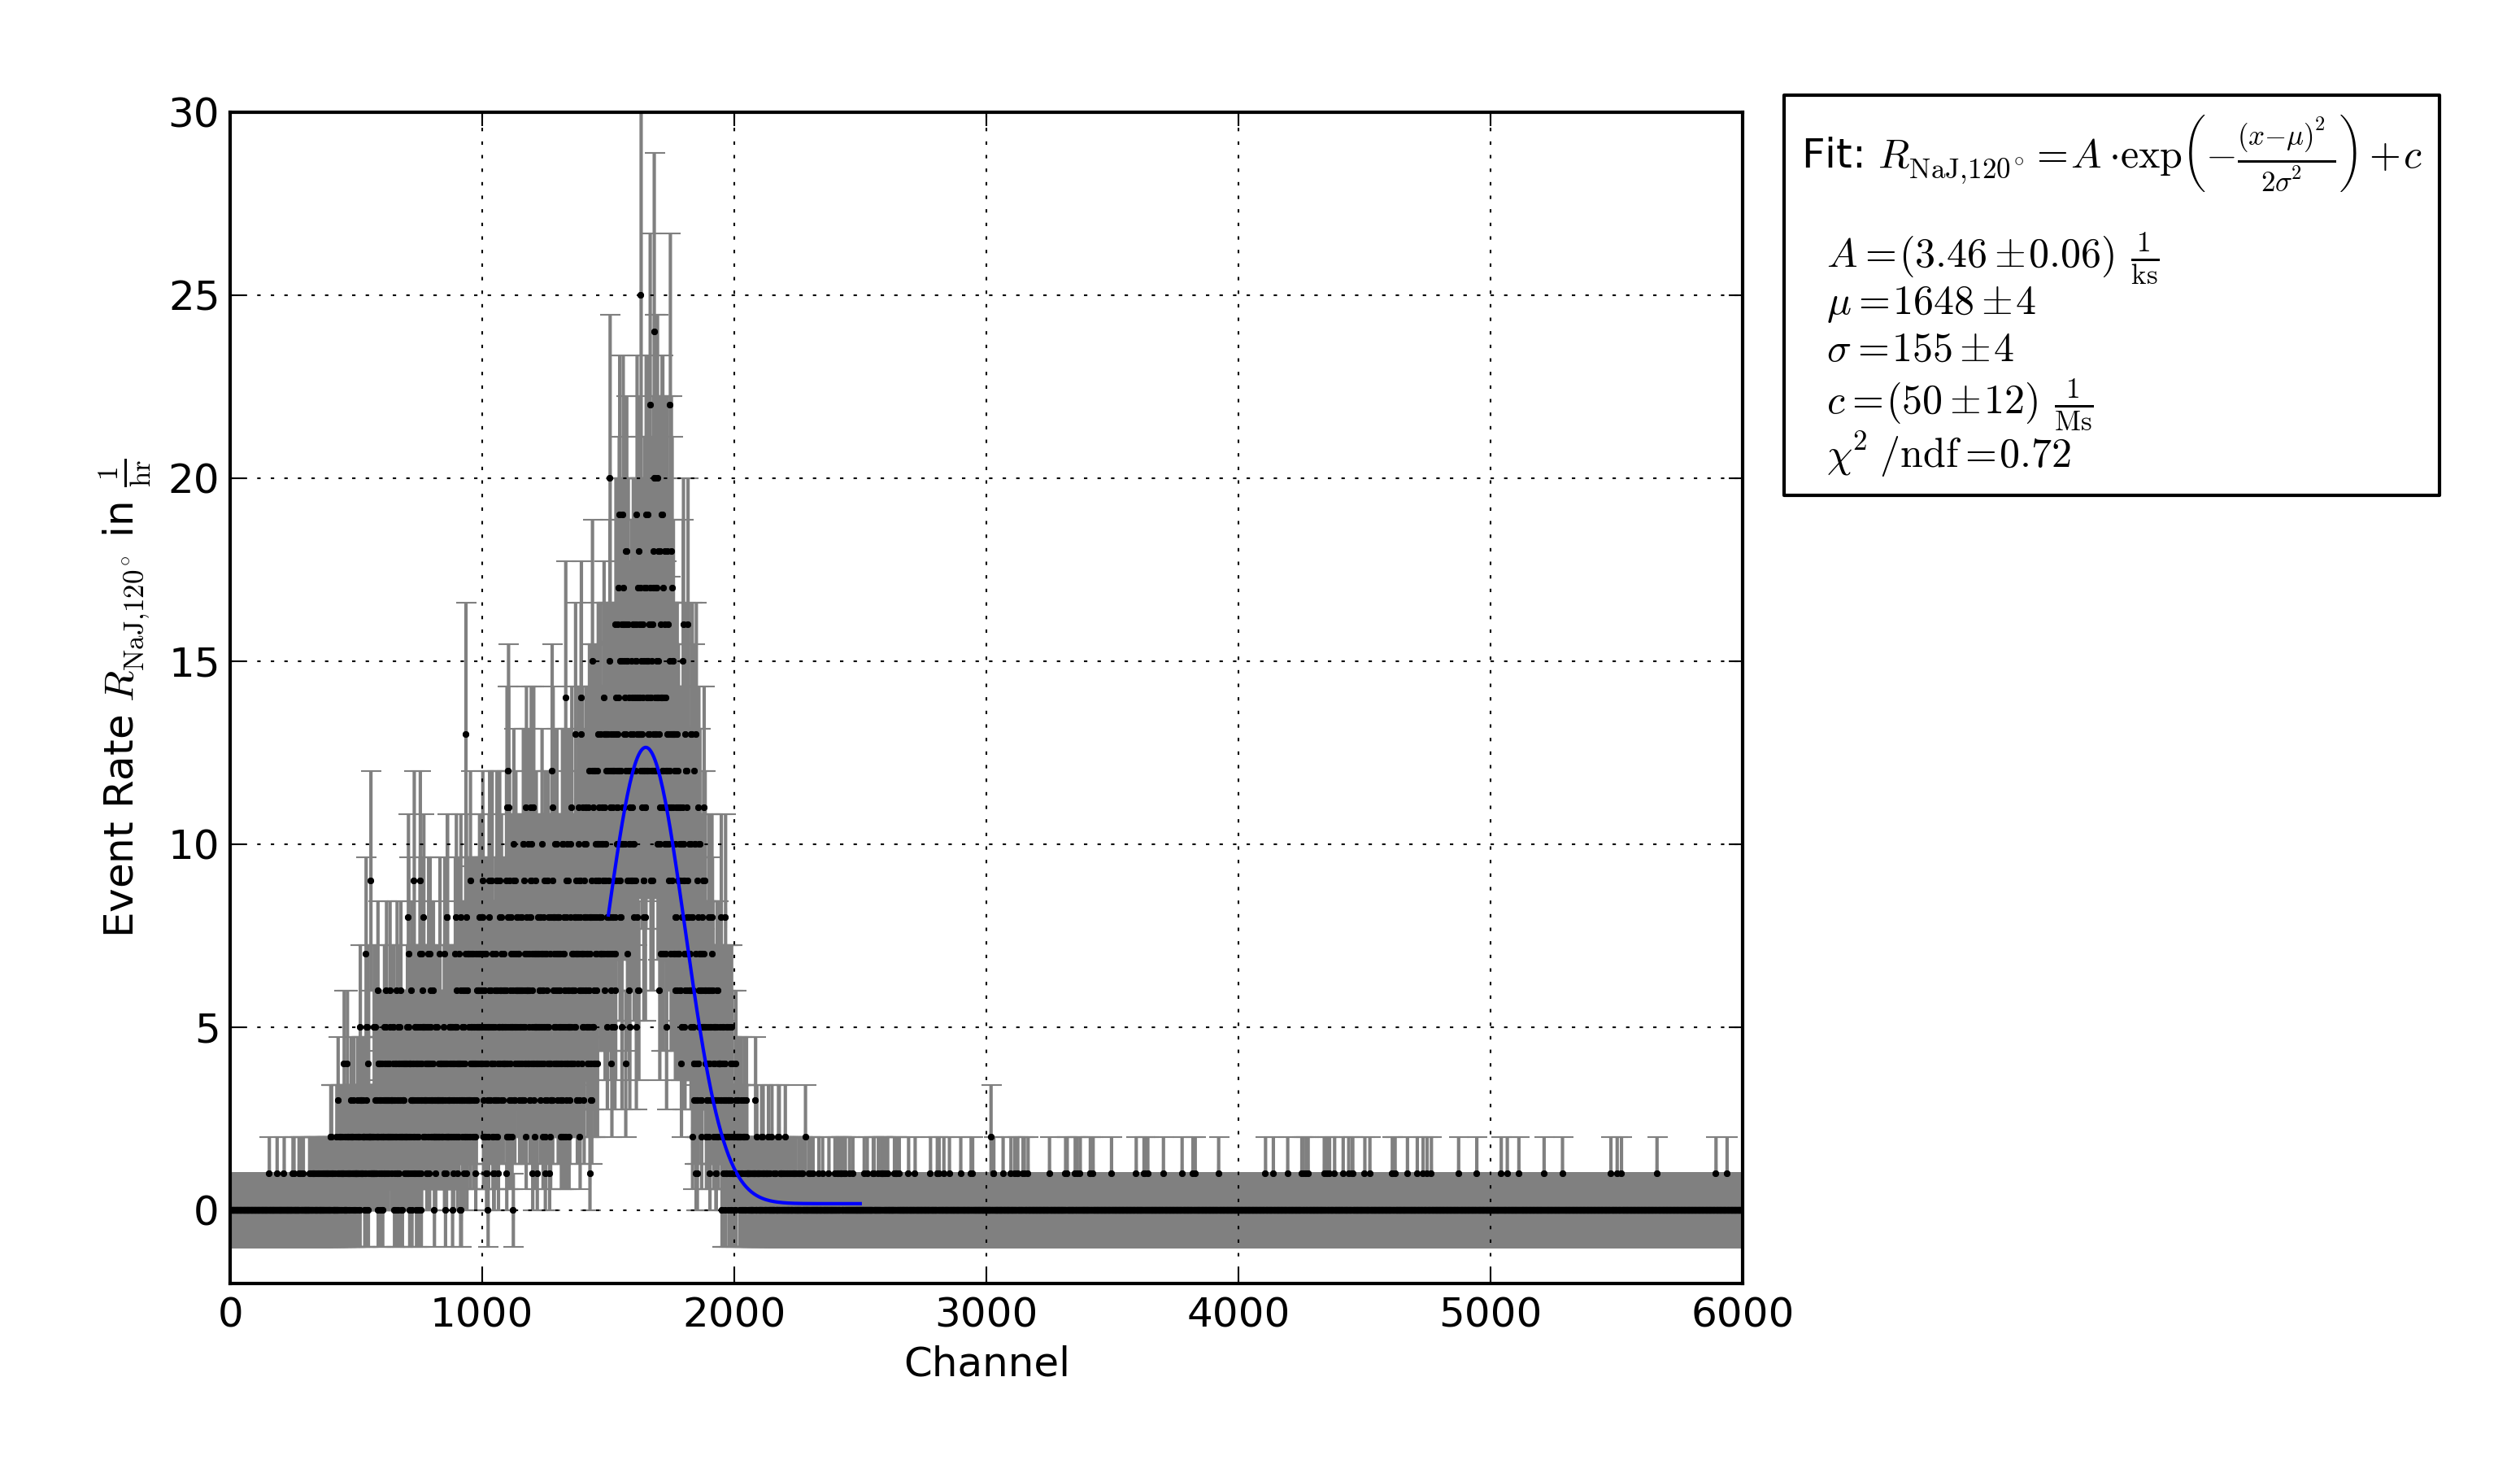
\includegraphics[width=0.6\textwidth]{plots/naj_120.png}
  \caption{Photon energy spectrum (NaI scintillator) of coincident signals
  with $\theta=120\degree$. Measurement duration $t=3600\mathrm{s}$.}
  \label{fig:naj120}
\end{figure}

\FloatBarrier
\subsection{Cross Section}
\begin{figure}[h!]
  \centering
  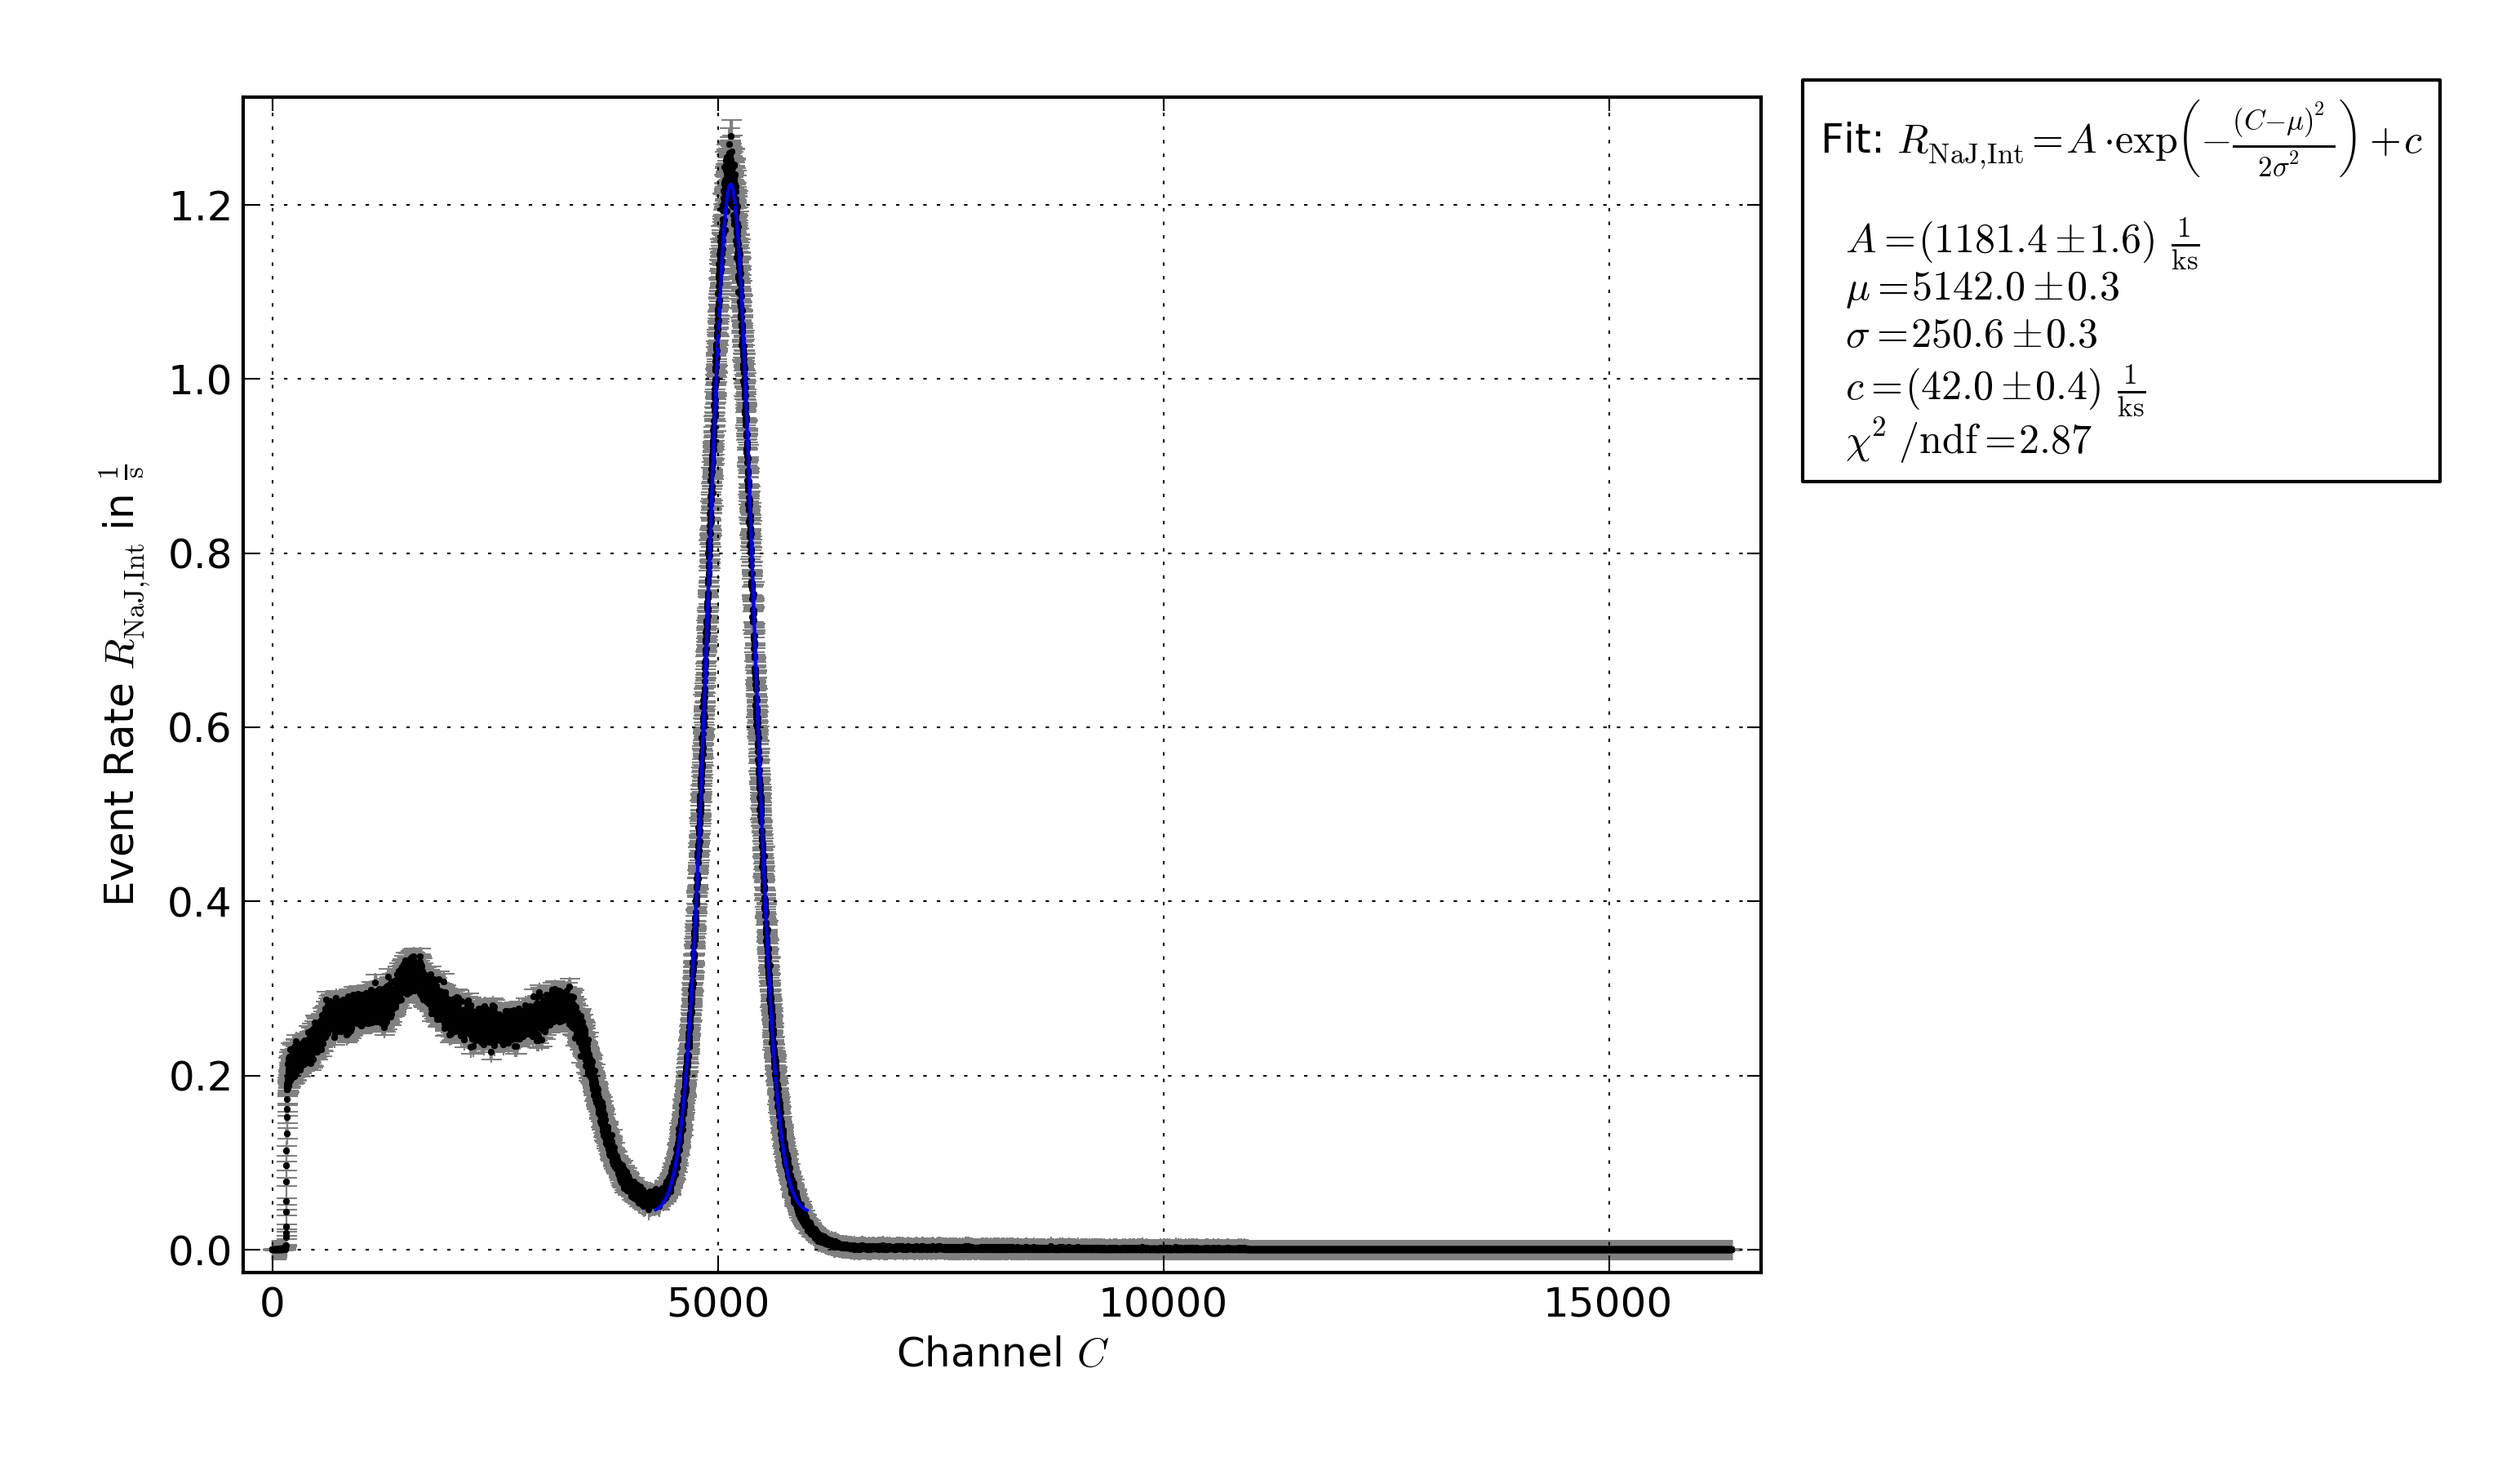
\includegraphics[width=0.6\textwidth]{plots/intensitaet.png}
  \caption{Direct \Cs spectrum measured with the NaI scintillator to determine
  the primary photon intensity. Measurement duration $t=3600\mathrm{s}$.}
  \label{fig:directI}
\end{figure}

\subsection{Notes}
The following pages show our notes we took during the measurement.

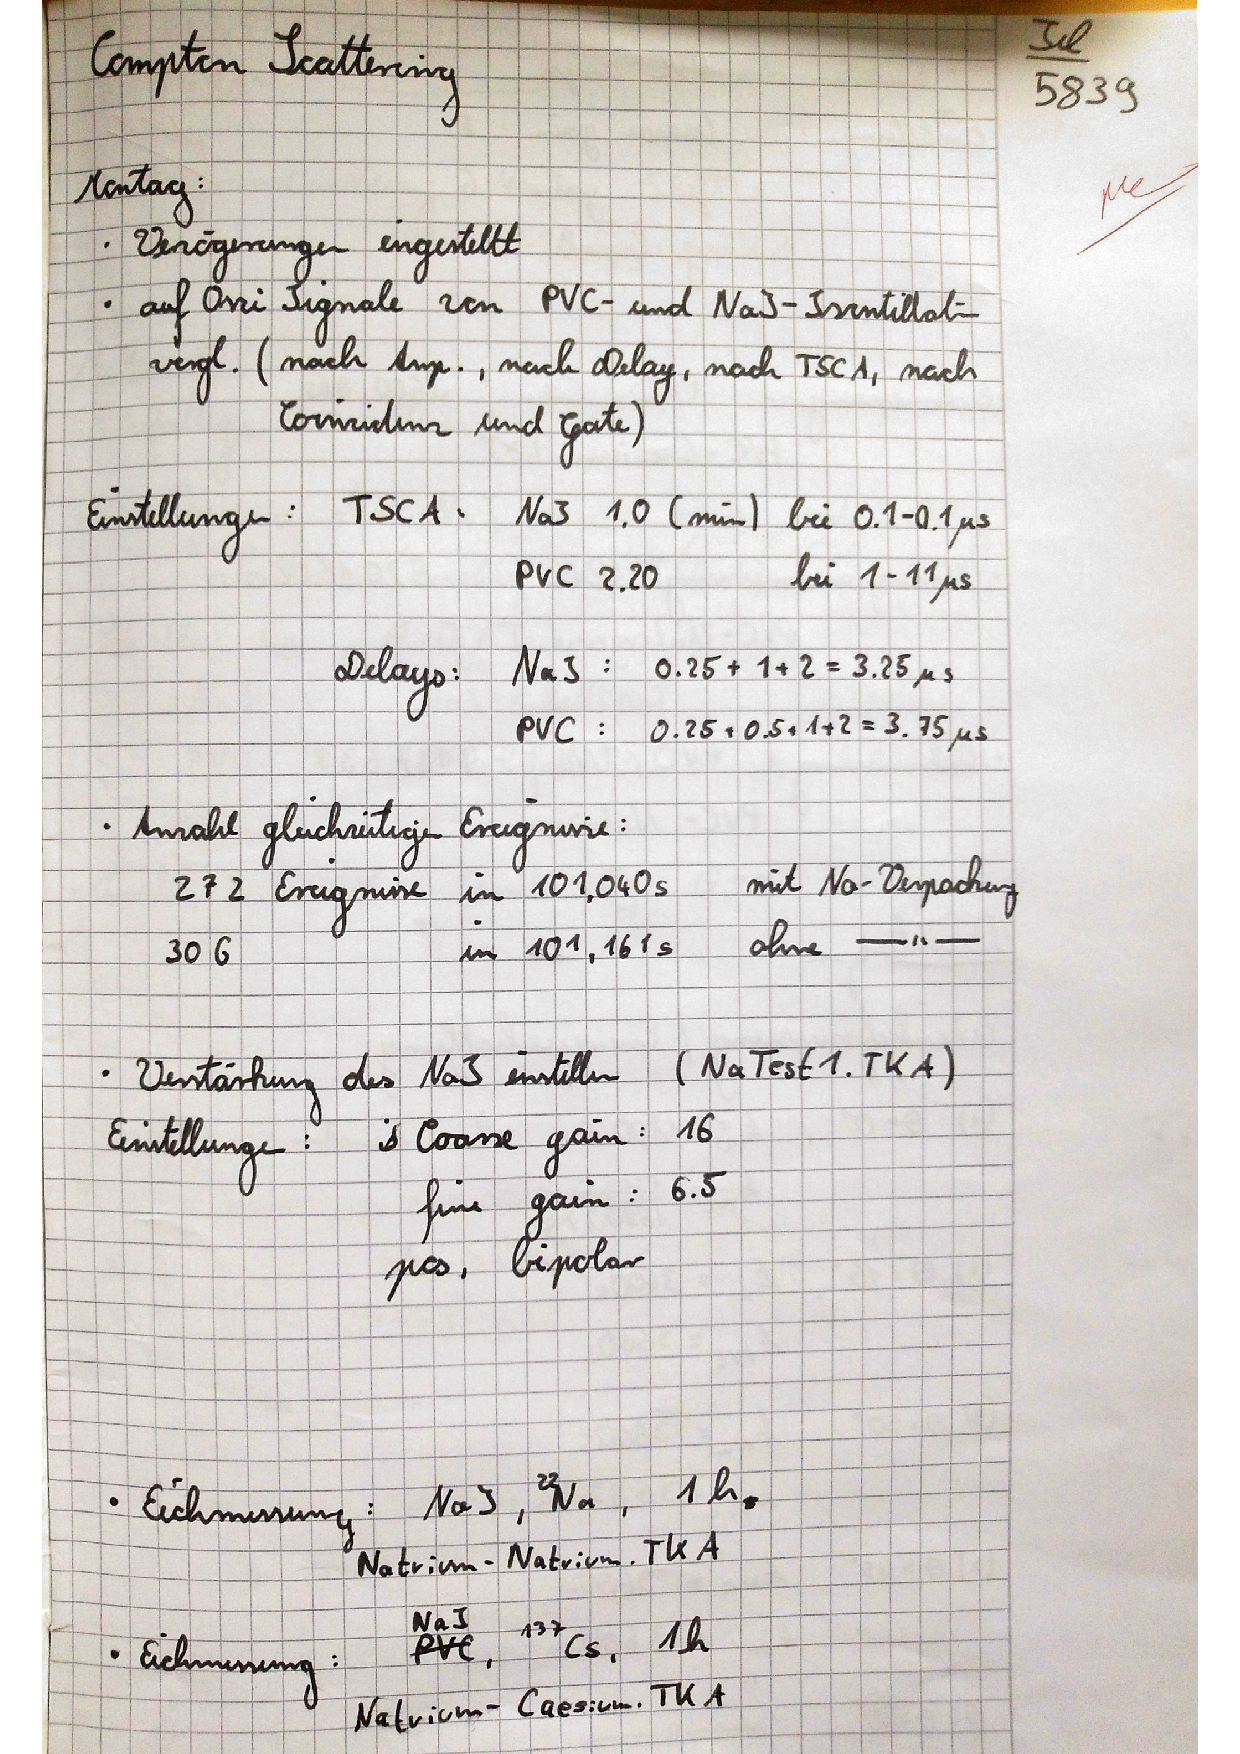
\includepdf[pages=-]{heft.pdf}
